% !TeX spellcheck = en_GB
\documentclass[a4paper, 11pt]{article}
%\documentclass[a4paper, 12pt]{article}
\usepackage[utf8]{inputenc}

%margin
\usepackage[margin=2cm]{geometry}
%\usepackage[margin=1in]{geometry}
\usepackage{changepage}
%line spacing
\renewcommand{\baselinestretch}{1.15}
%\renewcommand{\baselinestretch}{1.6}
%lists
\usepackage{enumitem}
%multi-columns
\usepackage{multicol}
%encoding
\usepackage[utf8]{inputenc}
\usepackage[T1]{fontenc}
%English
\usepackage[english]{babel}
%colors
\usepackage[dvipsnames,svgnames,table]{xcolor}
%tables
\usepackage{multirow}
\usepackage{longtable}
%for math
\usepackage{amsfonts}
\usepackage{amssymb}
\usepackage{mathrsfs}
\usepackage{amsmath}
\usepackage{amsthm}
\usepackage{mathtools}
\usepackage{nicefrac}
\usepackage{makecell}
%for images
\usepackage{graphicx}
\graphicspath{ {./img/} }
%for plots
\usepackage{tikz}
\usetikzlibrary{mindmap}
\usepackage{adjustbox}
%links
\usepackage[hyphens]{url}
\usepackage{hyperref}
%\hypersetup{colorlinks=true}
%citations
\usepackage[square]{natbib}
\bibliographystyle{unsrtnat}
%code
\usepackage{minted}
\usepackage{algpseudocode}
\definecolor{CodeColor}{RGB}{100, 100, 100}
%files tree architecture
\usepackage{dirtree}



%environments
\newtheorem*{notation}{Notation}
\newtheorem{definition}{Definition}[section]
\newtheorem{proposition}{Proposition}[section]
\newtheorem{property}{Property}[section]
\newtheorem{lemma}{Lemma}[section]
\newtheorem{theorem}{Theorem}
\newtheorem{corollary}{Corollary}[section]
\newtheorem{conjecture}{Conjecture}
%commands
%\newcommand{\name}[num]{definition}
\newcommand{\primes}{\mathbb{P}}
\newcommand{\N}{\mathbb{N}}
\newcommand{\Z}{\mathbb{Z}}
\newcommand{\Q}{\mathbb{Q}}
\newcommand{\D}{\mathbb{D}}
\newcommand{\R}{\mathbb{R}}
\newcommand{\C}{\mathbb{C}}
\newcommand{\F}{\mathbb{F}}
\newcommand{\halfplane}{\mathbb{H}}
%\newcommand{\dim}[1]{\text{dim}(#1)}
\newcommand{\SL}[2]{\text{SL}_{#1}(#2)}
\newcommand{\Norm}[2][]{\text{Norm}_{#1}(#2)}
\newcommand{\floor}[1]{\lfloor #1 \rfloor}
\newcommand{\ceil}[1]{\lceil #1 \rceil}
\newcommand{\abs}[1]{| #1 |}
\newcommand{\curt}[1]{\sqrt[3]{#1}}
\newcommand{\Ker}[1]{\text{Ker}(#1)}
\newcommand{\Image}[1]{\text{Im}(#1)}
\newcommand{\Gal}[1]{\text{Gal}(#1)}
\newcommand{\Frob}[2]{\text{Frob}_{#1}(#2)}
\newcommand{\Tr}[1]{\text{Tr}(#1)}
\newcommand{\Det}[1]{\text{Det}(#1)}
\newcommand{\End}[1]{\text{End}(#1)}
\newcommand{\Aut}[1]{\text{Aut}(#1)}
\newcommand{\legendre}[2]{\left( \frac{#1}{#2} \right)}
\newcommand{\degree}[1]{\partial #1}




\begin{document}
	\begin{titlepage}
	\newcommand{\HRule}{\rule{\linewidth}{0.5mm}}
		\begin{center}
		\includegraphics[scale=0.08]{ucl_logo.png}
		\vspace*{1cm}
		
		\textsc{\LARGE University College of London}\\[0.75cm]
		\textsc{\LARGE Department of Mathematics}
		
		\vspace{1.5cm}
		
		\HRule
%		\vspace{1cm}
%		
%		\textbf{\huge Modular Forms Modulo 2}
		\vspace{0.5cm}
		
		\textbf{\huge Modular Forms Modulo 2:\\}
		\vspace{0.3cm}
		\textbf{\huge Governing Fields for the Hecke Algebra}
		
		\vspace{0.5cm}
		\HRule
		
		\vspace{1.5cm}
		
		\begin{minipage}{0.4\textwidth}
			\begin{flushleft}
				\large
				\textit{Author}\\
				Paul \textsc{Dubois}
			\end{flushleft}
		\end{minipage}
		~
		\begin{minipage}{0.4\textwidth}
			\begin{flushright}
				\large
				\textit{Supervisor}\\
				Djordjo \textsc{Milovic}
			\end{flushright}
		\end{minipage}
		
		\vfill
		
		{\large March 12, 2020} 
	\end{center}
\end{titlepage}

	\begin{center}
		\LARGE Modular Forms Modulo 2
	\end{center}
	\vspace{0.5cm}
	\begin{abstract}
		Modular forms are functions over the upper half plane that play a prominent role in mathematics.
		Studying their properties over finite fields can yield useful information about the arithmetic of their Fourier coefficients.
		In this paper, we study modular forms over the smallest field of all, containing only an additive identity and a multiplicative identity, that is, $\F_2$.
		
		After introducing modular forms over the complex numbers, we will show how to reduce modular forms modulo 2.
		In this setting, modular forms may be seen as polynomials in the modular discriminant $\Delta$ or as power series in $q=\exp(2\pi i z)$. The duality between these two representations is crucial and we will use it in the development of a new computing technique: exact computations.
		
		We will then concentrate on the study of prime Hecke operators $T_p$ acting on modular forms modulo 2.
		These operators are nilpotent, with respect to a given modular form. The order of nilpotency is known, and we will discuss it.
		A Hecke operator $T_p$ at an odd prime $p$ acting on odd powers of $\Delta$ may also be expressed as power series in $T_3$ and $T_5$.
		
		The coefficient of $T_3^{i}T_5^{j}$ of this power series is denoted by $a_{ij}(p)$, and it will play a particularly important role in our study.
		The map $p \mapsto a_{ij}(p)$ is in fact Frobenian.
		We will try to discover new governing fields for these maps.
		
		In the last section, we will discuss the computing techniques developed to achieve the various computations performed.
	\end{abstract}
	\tableofcontents
	
	% !TeX spellcheck = en_GB
\setcounter{section}{-1}
\section{Introduction}

Our main goal will be to find new governing fields for the maps $a_{ij}$ involved in the expression of Hecke operators as power series of $T_3$ and $T_5$.
This will lead us to a new conjecture.



In section 1, we will introduce modular forms as functions of the upper half-plane.
We will present standard examples and basic properties of these modular forms.
Then we will define Hecke operators $T_n$ on modular forms.

Section 2 is dedicated to the reduction of modular forms modulo 2.
We will build up the theory and effectively perform this reduction.
We will do so first on modular forms, and then on the Hecke operators.
Our interest will be limited to Hecke operators for prime numbers ($T_p$).
It is important to determine if the reduction of Hecke operators modulo 2 becomes trivial.
In fact, it is never trivial.
We will prove this via the classical way, and as a consequence of a property that will be new to this paper.
As the reduction is not trivial, this yields an interesting theory.
We will, therefore, study the properties of Hecke operators modulo two.
The main one is that, given a modular form, Hecke operators are all nilpotent.
Finding the order of nilpotency of a modular form is a solved problem, that we will go through.

Section 3 is then dedicated to the Hecke algebra (the space of Hecke operators) modulo 2.
They are generated by power series of $T_3$ and $T_5$, and we will prove it.
The coefficients of this power series for $T_p$ are denoted $a_{ij}(p)$.
They will play a major role in the rest of the paper.

In section 4, we introduce all the algebraic number theory that will be needed for the rest of the paper.
First, we define the basis of algebraic number theory, that is field extensions, ideals, prime ideals, splitting, ramification and inertia.
Then we will look at Frobenius elements, together with their basic properties.
Finally, we mention Chebotarev's density theorem.

Then we will make the link between the last two sections (3 and 4): the coefficients $a_{ij}(p)$, seen as a map, are Frobenian.
The first cases (for small $i+j \leq 2$) have already been studied, and we know what the corresponding governing fields are.
Our goal is to investigate the possible governing fields for other cases (that is, for $i+j>2$).
We will analyse extensions numerically.
After this numerical analysis, we will come up with very strong candidates as governing fields for $a_{0k}(p)$ and $a_{k0}(p)$ for $k \leq 7$.
The potential governing fields are extensions of each other.
When drawing a diagram as in \ref{diagramFieldsExtensions}, they appear on the \textit{extreme sides}.
It appears that the Galois group of all diagonal governing fields that are found are dihedral groups.
The fact that this is verified not only for $k \leq 2$, but in fact $k \leq 7$ leads us to a new conjecture: the on diagonal governing groups \ref{diagonalGoverningGroupsConjecture}.

In the last section, we will discuss computational methods.
The results gave enough data to analyse the fields extensions, which was the goal of the paper.
To get this data, various techniques will be involved.
We will use the structure of the mathematical objects, together with careful programming to create a new computing technique (so-called "exact computations").
It allows, in the case of modular forms modulo 2, to recover the numerical error made when calculating Hecke operator of forms.
We will combine this with a high-performance language (Julia), and a high-performance library to compute fields extensions (PARI GP).

In the appendix, a subset of the tables from the computations made can be found.
The most important parts of the code used are also in the appendix.
Tables and code have their full versions available online (the corresponding links are in the appendix as well).
The governing fields calculated may be found at the very end of the appendix.

	% !TeX spellcheck = en_GB
\section{Modular forms}
\subsection{Modular forms of level 1}
Let $\halfplane$ denote the \textit{upper-half plane}, that is, 
$$\halfplane = \{z = x+yi \in \C | \ y>0 \}.$$
We say that a function $f:\halfplane 
 \C$ is \textit{weakly modular} of \textit{weight} $2k$ if $f$ is meromorphic and
$$
f(z) = (cz+d)^{-2k} f \left( \frac{az+b}{cz+d} \right)
\qquad \text{ for all }
\begin{pmatrix} a & b\\
				c & d
\end{pmatrix}
\in \SL2{\Z}.
$$
The group $\SL2{\Z}$ of invertible 2-by-2 matrices over $\Z$ with  is generated by
$$
S = \begin{pmatrix} 0 & -1 \\
					1 &  0
\end{pmatrix}
\quad \text{ and } \quad
T = \begin{pmatrix} 1 & 1 \\
					0 & 1 
\end{pmatrix};
$$
see \cite[p.1-2]{SL2Z}.
From this property, we can derive an alternative definition of weakly modular functions:
$f$ is weakly modular of weight $2k$ if $f$ is meromorphic and
$$
f(z+1) = f(z) \quad \text{ and } \quad f(-1/z) = z^k f(z),
$$
for all $z \in \C$.
Moreover, we define a function $f:\halfplane \mapsto \C$ to be \textit{modular} of weight $2k$ if $f$ is holomorphic and weakly modular.
Lastly, we say that a function $f:\halfplane \mapsto \C$ is a \textit{modular form} of weight $2k$ if it modular and holomorphic at $\infty$, that is, $f(\nicefrac{1}{z})$ is holomorphic at $z=0$.

It is straightforward to check, using the above definition, that the set of modular forms of weight $2k$ is closed under addition and multiplication by complex scalars.
More precisely:
\begin{itemize}
    \item If $f_1$ and $f_2$ are modular forms of weight $2k$, then $f_1+f_2: z \mapsto f_1(z)+f_2(z)$ is modular of weight $2k$ as well.
    
    \item Similarly, if $\lambda \in \C$ and $f$ is a modular form of weight $2k$, then so is $\lambda \cdot f: z \mapsto \lambda f(z)$.
\end{itemize}
Therefore, modular forms of weight $2k$ over $\C$ form a vector space. We denote it $M_k$.

It is also possible to multiply modular forms, in which case the weights are additive:
If $f_1$ and $f_2$ are modular forms of respective weights $2k_1$ and $2k_2$, then $f_1 \cdot f_2:z \mapsto f_1(z)f_2(z)$ is modular of weight $2k_1+2k_2$.

We deduce that we can take powers of modular forms, and the weight is then multiplied by the exponent:
if $f(z)$ is modular of weight $2k$, then $f^n(z)$ is modular of weight $2k \cdot n$ (with $n \in \N$ \footnote{The set of naturals $\N$ is taken to start from $0$ in this paper.} ).



\subsection{Typical Modular Forms}
\subsubsection{Eisenstein series $G_k$}
The most famous class of modular forms is probably the \textit{Eisenstein series}, usually denoted $G_k$. We define them as follows \cite[Examples of Modular Forms]{ModularFormsComputationalApproach}:
$$
G_k(z) = \sum_{(m,n) \in \Z^2\setminus\{(0,0)\}} \frac{1}{(mz+n)^{2k}}
$$
for $k \geq 2$.

It is easy to check that $G_k$ are modular of weight $2k$ \cite[Proposition 2.1]{ModularFormsComputationalApproach}, as:
$$
G_k(z+1) = G_k(z)
$$
(using $(m,n+m) \mapsto (m,n)$, an invertible map) and
$$
G_k(-1/z) = z^k G_k(z)
$$
(using $(m,-n) \mapsto (m,n)$, an invertible map).
It is pleasant to remark that \cite[Proposition 2.2]{ModularFormsComputationalApproach}
$$
G_k(\infty) = \sum_{n \in \Z \setminus \{0\} } \frac{1}{n^{2k}} = 2\zeta(2k),
$$ where $\zeta(k)$ is Riemann zeta function.
The values of this function are well-known on positive even numbers, and we deduce \cite[p.194]{MathHandbook} that:
$$
G_k(\infty) = 2\zeta(2k) = \frac{(2\pi)^{2k}}{(2k)!}B_k,
$$
where $B_k = (-1)^{k+1} b_{2k}$ and $b_k$ are Bernoulli numbers.

\subsubsection{The Modular Discriminant $\Delta$}
We will be interested in one main modular form in the rest of this article: the \textit{modular discriminant} $\Delta$.
We define $\Delta$ in terms of $G_k$ as follows \cite[p.84]{CourseInArithmetic}:
$$
\Delta = \left( \frac{1}{(2\pi)^{12}} \right) (g_2^3 - 27g_3^2) \in M_6 \qquad \text{ with } g_2 = 40G_2 \text{ and } g_3 = 140G_3
$$
As $g_2^3$ is modular of weight $4 \cdot 3=12$ and $g_3^2$ of weight $6 \cdot 2 = 12$, $\Delta$ is modular of weight $12$.
Multiplying by the scalar $\left( \nicefrac{1}{(2\pi)^{12}} \right)$ doesn't change the weight of the modular form, and it will we useful later for normalization purposes.

Now, using 
$
G_2(\infty) = 2\zeta(4) = \frac{\pi^4}{45}
$
 and 
$
G_3(\infty) = 2\zeta(6) = \frac{2\pi^4}{945}
$
, we get 
$$
\Delta(\infty) = \left( \frac{1}{(2\pi)^{12}} \right) \left[ \left( \frac{4\pi^4}{3} \right)^3 - \left( \frac{8\pi^4}{27} \right)^2 \right] =  0
$$
so $\Delta$ has a zero at infinity.


\subsection{Cusp Forms}
A function $f:\halfplane \to \C$ that is a modular form may in addition be a \textit{cusp form}, if $f(\infty)=0$.
We will denote the \textit{space of modular cusp forms} of weight $2k$ over $\C$ by $M_k^0$. This space of cusp forms of weight $2k$ is a subset of the space of modular forms of weight $2k$.

It is useful to note $G_k(\infty) = \sum_{n \in \N^*} \frac{2}{n^{2k}} > 2$ and in particular, $G_k(\infty) \neq 0$, so $G_k$ are \textit{not} cusp forms for any $k$.
As we have shown it before, $\Delta(\infty)=0$, so $\Delta$ is a modular cusp form of weight 12, so $\Delta \in M_6^0$.
Using tools from complex analysis, we can prove that $\Delta$ has only one zero (at infinity), which has order one \cite[p.88]{CourseInArithmetic}.

We have the following relation:
\begin{theorem}
	\cite[p.88]{CourseInArithmetic}:
    $M_k \cong M_k^0 \oplus \C \cdot G_k \quad \text{ for all } k \geq 2$
\end{theorem}
\begin{proof}
    We let $\Phi:M_k \to \C$ such that if $f \in M_k$, $\Phi(f) = f(\infty)$.
    Now, we have $\Ker{\Phi} = M_k^0$, therefore, by the 1\textsuperscript{st} Isomorphism Theorem, $\nicefrac{M_k}{M_k^0} \cong \Image{\Phi} \subseteq \C$.
    Note that $G_k \in M_k$, and $G_k(\infty) = \sum_{n \in \Z^*} \frac{1}{n^{2k}} \neq 0$, so $G_k \not\in M_k^0$.
    As $G_k \neq 0$, $\dim(\nicefrac{M_k}{M_k^0}) \geq 1$ and $\Image{\Phi} = \C$.
    Thus, $G_k \in M_k \setminus M_k^0$.
    
    Finally, we have $M_k \cong M_k^0 \oplus \C \cdot G_k$ if $k \geq 2$.
    (The above argument fails for $k<2$ as $G_k$ is not well defined any more.)
\end{proof}
Therefore, the dimensions of $M_k$ and $M_k^0$ are closely linked.



\subsection{Dimensions of Spaces of Modular Forms}
The fact that multiplying two modular forms gives a function that remains modular yields that we may map a set of modular forms to another.

\begin{theorem}\cite[p.88]{CourseInArithmetic}.
	We have $M_{k-6} \cong M_k^0$.
\end{theorem}
\begin{proof}
    We define $\Phi:M_{k-6} \to M_k^0$ by setting, 
    $$\Phi(f)(z) = \Delta(z)f(z) \quad \text{ for } f \in M_{k-6}.$$
    This is well defined as if $f$ has weight $2(k-6)$, $\Delta \cdot f$ has weight $2k$ since $\Delta$ has weight $12$. As $\Delta$ is a cusp from, $\Delta \cdot f$ will also be a cusp form.
    From the definition, $\Phi$ is a linear map.
    
    Now, if $g \in M_k^0$, we may define $\Psi: M_k^0 \to M_{k-6}$ by setting
    $$\Psi(g)(z) = \nicefrac{g(z)}{\Delta(z)} \quad \text{ for } g \in M_k^0.$$
    This is well defined as if $g$ has weight $2k$, $\Delta \cdot f$ has weight $2k$ since $\Delta$ has weight $12$.
    This is well defined as $\Delta$ has only one zero, at infinity, where $g$ also has a zero (as $g$ is a cusp form). The weights agree again as well.
    We remark that $\Psi = \Phi^{-1}$. So $\Phi$ is bijective, and thus an isomorphism. 
    Finally, we have $M_{k-6} \cong M_k^0$.
\end{proof}
This theorem, combined with the previous one is very powerful: it shows that there must be a pattern in the sequence of dimensions $\dim(M_k)$ and $\dim(M_k^0)$ for $k \geq 2$.
We have $M_k \cong M_k^0 \oplus \C \cdot G_k \cong M_{k-6} \oplus \C \cdot G_k$, so $\dim(M_k) = \dim(M_{k-6})+1$ when $k \geq 2$.
Thus, if we compute the dimensions of $M_0$, $M_1$, $M_2$, $M_3$, $M_4$, $M_5$, we can extrapolate dimensions of $M_k$ and $M_k^0$ for all $k$.

Using complex analysis techniques again, we have:
\begin{itemize}
    \item $\dim(M_k) = 0 \text{ for } k < 0$
    \item $\dim(M_1) = 0$
    \item $\dim(M_0) = \dim(M_2) = \dim(M_3) = \dim(M_4) = \dim(M_5) = 1$
\end{itemize}
%[proof?]
In the case $k=0$, $\dim(M_0) = 1$. As $f(z) = 1$ is clearly a modular from of weight $0$, $\{1\}$ is a basis for $M_0$. We deduce $\dim(M_k^0) = 0$ as $1$ is clearly not a cusp form.
In the case $k=1$, $\dim(M_1) = 0$, which makes $\dim(M_1^0) = 0$ automatically.
(Cases $k<0$ are similar to $k=1$.)

Other cases may be derived directly from the relations (using induction to get general formulas), and we obtain:

%[Table of dimensions of $M_k$ and $M_k^0$]
\begin{center}
\begin{tabular}{||c||c|c|c||} 
    \hline
    Space & $k<0$ & $k \geq 0, \ k \equiv 1 \bmod 6$ & $k \geq 0, \ k \not \equiv 1 \bmod 6$ \\
    \hline
    \hline
    $\dim(M_k)$ & $0$ & $\floor{\nicefrac{k}{6}}$ & $\floor{\nicefrac{k}{6}} + 1$ \\
    \hline
    $\dim(M_k^0)$ & $0$ & $\max\{0, \floor{\nicefrac{k}{6}} - 1\}$ & $\floor{\nicefrac{k}{6}}$ \\
    \hline
\end{tabular}
\end{center}
Note that the $\max$ is taken only to avoid negative dimensions.



\subsection{Fourier Expansion}
\subsubsection{Definition}
To study modular forms, we can use Fourier expansion.
As a modular form $f$ satisfies $f(z) = f(z+1)$ for all $z \in \C$, we can express the Fourier expansion in terms of $q = e^{2 \pi i z}$.
Thus, in the case of $f$ being a modular form of weight $2k$, 
a \textit{Fourier expansion} is a representation of $f$ as a power series of $e^{2\pi i n z}$
i.e. $$f(z) = \sum_{n \in \Z} a_n(f) e^{2\pi inz}.$$
We usually denote $q = e^{2\pi i z}$ so that $q^n = e^{2\pi i n z}$ 
and the Fourier expansion of $f$ become 
$$
f(q) = \sum_{n \in \Z} a_n(f) q^n.
$$
When in this form, we may as well call it the \textit{$q$-expansion}.

\paragraph{Asymptotic Notation}
The asymptotic behaviour of a function may be expressed in terms of another.
This is done via the \textit{big-O notation} or \textit{asymptotic notation}.
We write $f(x) = \mathcal{O}(g(x))$ as $x \mapsto a$ if there exist $\delta, M \in \R$ such that $\abs{f(x)} \leq Mg(x)$ when $0 < \abs{x-a} \leq \delta$.
For example, if $a=0$ (which will always be the case in here), we have that if $\alpha \geq \beta$, then $x^{\alpha} = \mathcal{O}(x^{\beta})$.

It will sometimes be useful to write the Fourier expansions only up to some coefficient.
For the $q$-series up to $m$, we will write $\mathcal{O}(q^m)$.
That is, if
$$
f(q) = \sum_{n \in \N} c(n) q^n,
$$
then
$$
f(q) = \sum_{n = 0}^{m-1} c(n) q^n \ + \mathcal{O}(q^m).
$$


\subsubsection{Typical Modular Forms Fourier Expansion}
\paragraph{Fourier Expansions of $G_k$}
The modular forms $G_k$ have the following $q$-expansion \cite[p.92]{CourseInArithmetic}:
$$
G_k(q) = 2\zeta(2k) + 2 \frac{{(2 \pi i)}^{2k}}{(2k-1)!} \sum_{n=1}^{\infty} \sigma_{2k-1}(n)q^n,
$$
where $\sigma_d$ is the generalized divisor function defined by:
$$
\sigma_d(n) = \sum_{m \mid n} m^d.
$$

\paragraph{Fourier Expansion of $\Delta$}
We also have \cite[p.95]{CourseInArithmetic}:
$$
\Delta(q) = q \prod_{n=1}^{\infty} (1-q^n)^{24}.
$$



\subsection{A Basis for Modular Forms}
\label{BasisModularForms}
We established that $M_k$ form a vector space over the complex numbers. 
One may ask then a basis for this vector space.

We would like to find a basis for each vector space $M_k$. It turns out that the modular forms $G_2$ and $G_3$ introduced before in fact generate a basis for all $M_k$. 
It is not obvious and may in fact seem wrong at a first glance: $G_2$ and $G_3$ are modular forms of weight $4$ and $6$, whereas $M_k$ in general have modular forms of weight $2k$.
However, by taking combinations of $G_2$ and $G_3$, we may obtain modular forms of any weight $2k$. It is important to remember that when multiplied, the weight of modular forms add up.

\begin{theorem}\cite[Theorem 2.17]{ModularFormsComputationalApproach}.
    The set $S = \{G_2^aG_3^b \mid a,b \in \N \footnote{In this paper, $0 \in \N$, i.e. $\N = \{ 0, 1, 2, 3, 4, \dots \}$.}, 2a+3b = k\}$ is a basis for $M_k$. 
\end{theorem}
\begin{proof}
    Of course, the cases when $\dim(M_k)=0$ (for $k<0$ and $k=1$) are trivial, as the basis is empty, and $2a+3b = k$ has no solution for $a,b \in \N$.
    To show $S$ is a basis, we need it to span $M_k$ and to be linearly independent.
    
    We start with spanning, and we proceed by induction on $k$, with step $6$.
    As $\dim(M_k)=1$ for $k=0,2,3,4,5,7$, and the equation $2a+3b = k$ has exactly one solution for $a,b \in \N$ (namely $(a,b)=(0,0), (1,0), (0,1), (2,0), (1,1), (2,1)$), $S$ has only one element, which must be the basis.
    Now, for $k>7$, take some $a,b \in \N$ such that $2a+3b=k$. Let $f \in M_k$, and $g = G_2^aG_3^b \in M_k$.
    We have$g(\infty) \neq 0$ as none of $G_2$ or $G_3$ is a cusp form. 
    So there must be a complex $\lambda$ such that $f - \lambda g$ is a cusp form. 
    Then $f - \lambda g \in M_k \cong M_{k-6}^0$ and we can find a $h \in M_{k-6}^*$ such that $h \cdot \Delta = f - \lambda g$.
    
    By induction, $h$ must be a polynomial of $G_2$ and $G_3$; by definition, $\Delta$ is one as well (note that yet, we don't put any restriction on powers of $G_2$ and $G_3$, other then being positive integers).
    Therefore, $f = \Delta \cdot h + \lambda g$ is a polynomial of $G_2$ and $G_3$.
    From the fact that $f \in M_k$ (i.e. $f$ has weight $2k$), terms of $f$ as a polynomial of $G_2$ and $G_3$ have the from $G_2^aG_3^b$ with $2a+3b=k$.
    
    We now want to show linear independence, we proceed by contradiction.
    Suppose there is a non-trivial linear relation of terms $G_2^aG_3^b$. 
    We can multiply it by suitable $G_2$ and $G_3$ so that all terms have the form $2a+3b = k \equiv 0 \bmod 12$.
    Then, we can divide all terms by $G_3^2$, witch gives us that there is a polynomial for which $\nicefrac{G_2^3}{G_3^2}$ is a root.
    In particular, this polynomial is constant when $\nicefrac{G_2^3}{G_3^2}$ is plugged.
    This contradicts the fact that $q$-expansion of $\nicefrac{G_2^3}{G_3^2}$ is not constant.
\end{proof}

This set of makes to be a basis, and one may even find it pleasant: given the two modular forms $G_2$ and $G_3$, this set generates all the modular forms of weight $2k$ that we could think of, if we only knew these two modular forms.



\subsection{Hecke Operators}
\label{DefHeckeOperators}
We define the \textit{Hecke operators} for a modular form $f$ as follows \cite[p.100]{CourseInArithmetic}:
$$
T_nf(z) = n^{2k-1}\sum_{a \geq 1,\, ad=n,\, 0 \leq b < d} d^{-2k}f \left( \frac{az+b}{d} \right)
$$
with $n \in \N$.
We can check that $T_nf$ is modular if $f$ is (as the sum of modular forms).
We may as well write $T_nf$ as a $q$-expansion as follows \cite[p.100]{CourseInArithmetic}: if $f(z) = \sum_{n \in \Z} c(n)q^n$, then
$$
T_nf(z) = \sum_{m \in \Z} \gamma(m)q^m
\quad \text{ with } \quad 
\gamma(z) = \sum_{a | (n,m),\, a \geq 1} a^{2k-1} c\left( \frac{mn}{a^2} \right).
$$

	% !TeX spellcheck = en_GB
\section{Modular Forms Modulo Two}
\subsection{Strategy to Reduce Modulo Two}
It is not trivial, at this point, why and how we can reduce modulo 2 modular forms, objects that have coefficients in $\C$.
In general, reduction modulo a number is only possible with whole numbers (integers).
We would like to reduce modulo 2 coefficients of the Fourier series for modular forms.
But at the moment, they lie in $\C$.

In fact, we will introduce a new basis for the modular forms: the so called Miller Basis.
The coefficients of all the forms in this basis are integers. It is then possible to consider the space of modular forms over $\Z$ instead of $\C$.
Once this is done, we will reduce all the newly integral coefficients modulo $2$.

In this section, we will denote all objects reduced modulo 2 with an $\overline{\text{over-line}}$:
\begin{itemize}
	\item The modular form $f$ once reduced will be denoted $\overline{f}$.	\item The coefficients of the $q$-expansion $c$ will reduce to $\overline{c}$
	\item The Hecke operators $T_n$ reduced will be denoted $\overline{T_n}$.
\end{itemize}

\subsection{Integral Basis}
\subsubsection{Normalisation of Typical Modular Forms}
\paragraph{Normalisation of Eisenstein series $G_k$}
We first recall the formula for $q$ extension of $G_k$ and the one for $\zeta(2k)$:
$$
G_k(q) = 2\zeta(2k) + 2 \frac{{(2 \pi i)}^{2k}}{(2k-1)!} \sum_{n=1}^{\infty} \sigma_{2k-1}(n)q^n
$$
and
$$
2\zeta(2k) = \frac{(2\pi)^{2k}}{(2k)!}B_k,
$$
so overall:
$$
G_k(q) = \frac{(2\pi)^{2k}}{(2k)!}B_k + 2 \frac{{(2 \pi i)}^{2k}}{(2k-1)!} \sum_{n=1}^{\infty} \sigma_{2k-1}(n)q^n.
$$

We would like to normalize this series, so that the coefficients become integers, so that we can ultimately reduce them modulo 2.
Right now, coefficients are rational.

As we want to keep the series modular with same weight, the only tool we have to normalize the series is multiplication by a constant.
The normalization is a crucial point: if we multiply by $2$ all coefficients of a modular form that already lie in $\Z$, the reduction modulo 2 will always give zero.

First, let's normalize the series to have particular values on some coefficients of interest.
There are two justified ways to do so: normalize to have constant ($q^0$) coefficient set to one, and to have $q^1$ coefficient set to one.
We will introduce both:
We define $E_k$ be such that:
$$
E_k \cdot 2\zeta(2k) = G_k,
$$
so that
$$
E_k = 1 + (-1)^k \frac{4k}{B_k} \sum_{n=1}^{\infty} \sigma_{2k-1}(n)q^n.
$$
$E_k$ then has constant coefficient set to 1.

We also define $F_k$ be such that:
$$
F_k \cdot \left( 2 \frac{{(2 \pi i)}^{2k}}{(2k-1)!} \right) = G_k,
$$
so that
$$
F_k =  (-1)^k \frac{B_k}{4k} + \sum_{n=1}^{\infty} \sigma_{2k-1}(n)q^n.
$$
$F_k$ then has $q$-coefficient set to 1 (as $\sigma_{2k-1}(1)=1$).

Clearly, the coefficients of this expansion remain in $\Q$ at least, and we will show that for some specific $k$, the coefficients lie in fact in $\Z$.
Both $F_k$ and $E_k$ are interesting, but for our purpose (reducing modulo 2), we will use $E_k$.
Note that $E_k$ are normalized versions of Eisenstein series $G_k$, but in literature, both are called Eisenstein series; see \cite[p.6]{IntoductionModularFormsWorkshop} for example.

\paragraph{The Modular Discriminant $\Delta$ Normalized}
Again, we recall the formula for $q$ extension of $\Delta$:
$$
\Delta(q) = q \prod_{n=1}^{\infty} (1-q^n)^{24}.
$$
Clearly, the coefficients in expansion of $\Delta$ are integers (which we can reduce modulo 2).
This is the reason why we defined $\Delta$ with the $\frac{1}{(2\pi)^{12}}$ factor in front.


\subsubsection{Miller Basis}
\paragraph{Basis with Integral Coefficients (in Fourier Series)}
Applying normalization $G_k \mapsto E_k$ above for $k=2,3$, we get:
\begin{align*}
	E_2 &= 1 + \frac{8}{B_2} \sum_{n=1}^{\infty} \sigma_{3}(n)q^n \qquad B_2 = \frac{1}{30} \\
	    &= 1 + 240 \sum_{n=1}^{\infty} \sigma_{3}(n)q^n
\end{align*}

and
\begin{align*}
	E_3 &= 1 - \frac{12}{B_3} \sum_{n=1}^{\infty} \sigma_{5}(n)q^n \qquad B_3 = \frac{1}{42} \\
	    &= 1 - 504 \sum_{n=1}^{\infty} \sigma_{5}(n)q^n
\end{align*}

Now, we have shown that $\{G_2^aG_3^b \mid 2a+3b=k\}$ is a basis for modular forms of weight $2k$ over the complex (see \ref{BasisModularForms}).
As $E_2 = \lambda G_2,\ \lambda \in \C$ and $E_3 = \mu G_3,\ \mu \in \C$, we have that $\{E_2^aE_3^b \mid 2a+3b=k\}$ remains a basis for $M_k$ over $\C$.

It is clear, from the series, that coefficients of the $q$-expansion of both $E_2$ and $E_3$ are all integers.
Thus, so are coefficients of combinations of $E_2$ and $E_3$.
Therefore, we have found a basis for $M_k$ such that all elements in the basis have only integral coefficients in their $q$-expansion.
\label{IntegralBasisModularForms}

\paragraph{Miller Basis for $M_k^0$}
This is a nice result, but we can in fact do better, by forcing the first coefficients to chosen values.

\begin{theorem}
	For the space of modular cusp forms $M_k^0$, there exists a basis $\{f_1, \cdots, f_r\}$ such that:
	\begin{itemize}
		\item $f_i \in \Z[[q]]$
		\item $ a_i^j = \delta_{ij} = 
		\left\lbrace
		\begin{array}{l l}
			1 & \text{ if } i   =  j \\
			0 & \text{ if } i \neq j
		\end{array}
		\right. \quad
		\forall 1 \leq i,j \leq r$\\
		where $a_i^j$ is the coefficient of $q^j$ in expansion of $f_i$.
	\end{itemize}
\end{theorem}
This is commonly called the Miller basis for $M_k^0$, as it was first introduced by Victor Saul Miller \cite{MillerThesis}.
\begin{proof}
	\begin{itemize}
		%boring part
		\item For $k<6$, $k=7$, we have $\dim(M_k^0)=0$.
		Thus, $\emptyset$ is a basis which satisfies the Miller basis properties.
		
		%semi-boring part
		\item For $k=6$, we have $\dim(M_k^0)=1$.
		Thus, $\{ \Delta \}$ is a basis which satisfies the Miller basis properties.
		
		%interesting part
		\item For $k \geq 7$, we let $r = \dim(M_k^0) \geq 1$.	
		We then consider the set $\{ g_j \mid 1 \leq j \leq r \}$ where
		$$
		g_j = \Delta^jE_3^{2(d-j)+b}E_2^a
		$$
		with $2a+3b \leq 7$, $2a+3b \cong k \bmod 6$ and $d = \frac{k-(2a+3b)}{6} \in \N$ (with $k \geq 7$).
		Note that $a$ and $b$ are unique unless $k \cong 0 \bmod 6$. In witch case, we use by convention $a=0$, $b=0$.
		As all $E_2$, $E_3$, and $\Delta$ have integral coefficients, $g_j$ will as well.
		
		We then look at the $q$-series
		$$
		\Delta(q) = q + \mathcal{O}(k^2) \implies \Delta^j(q) = q^j + \mathcal{O}(k^{j+1}).
		$$
		As we normalized, we have
		$$
		E_2(q) = 1 + \mathcal{O}(q) \implies E_2^{\alpha}(q) = 1 + \mathcal{O}(q)
		$$
		$$
		\text{ and } E_3(q) = 1 + \mathcal{O}(q) \implies E_3^{\alpha}(q) = 1 + \mathcal{O}(q).
		$$
		
		This gives:
		$$
		g_j(q) = q^j + \mathcal{O}(q^{j+1}) \quad \forall 1 \leq j \leq r.
		$$
		Therefore, $\{ g_j \mid 1 \leq j \leq r \}$ is clearly a linearly independent set. By dimension argument, it also spans $M_k^0$. Therefore, it forms a basis.
		Moreover, in this basis: $a_i^j = \delta_{ij} \quad i \leq j$.
		
		Now, viewing $\Delta$-coefficients of the modular forms $\{g_j\}$ as rows of a matrix, we can perform Gaussian elimination on them.
		We will obtain a basis $\{f_j \mid 1 \leq j \leq r \}$ such that: $a_i^j = \delta_{ij} \text{ for all } 1 \leq i,j \leq r$.
		The coefficients will remain in $\Z$.
	\end{itemize}
\end{proof}

\paragraph{Extension to all $M_k$}
We already have a basis for $M_k^0$, as $\dim(M_k) = \dim(M_k^0) + 1$ (over $\C$), we just need to adjoint one element of $M_k \setminus M_k^0$ to our basis.
It was shown before that $\{E_2^aE_3^b \mid 2a+3b=k\}$ is a basis for $M_k$ with integral coefficients (see \ref{IntegralBasisModularForms}).
One may see from the $q$-expansion that $E_2^aE_3^b = 1 + O(q)$ so $E_2^aE_3^b \in M_k \setminus M_k^0$.
Therefore, we can just add one element of $\{E_2^aE_3^b \mid 2a+3b = k\}$ to the Miller basis, and use Gaussian elimination again.
We get a basis for $M_k$ of the form $\{f_j \mid 0 \leq j \leq r \}$ such that in this basis: $a_i^j = \delta_{ij} \text{ for all } 0 \leq i,j \leq r$ (with $r=\dim(M_k^0)$ i.e. $r+1=\dim(M_k)$).

\paragraph{Miller Basis Examples}
\subparagraph{Miller basis for $k=16$}
We can calculate the Miller basis for $k=16$:
$k \cong 4 \bmod 12$ so $a=2$ and $b=0$; $d=2$.
We put $g_1 = \Delta^1E_3^2E_2^2$, so:
\begin{align*}
    g_1(q) &= \Delta(q)E_2^2(q)E_3^2(q)\\
           &= \left[ q - 24q^2 + 252q^3 + O(q^4) \right]\\
           & \qquad \cdot \left[ 1 + 240q + 2160q^2 + 6720q^3 + O(q^4) \right]^2\\
           & \qquad \qquad \cdot \left[ 1 - 504q - 16632q^2 + 122976q^3 + O(q^4) \right]^2\\
           &= q - 552q^2 - 188244q^3 + O(q^4)
% (Wolfram|Alpha) develop (q - 24q^2 + 252q^3)(1 + 240q + 2160q^2 + 6720q^3)^2(1 - 504q - 16632q^2 + 122976q^3)^2
\end{align*}
and $g_2 = \Delta^2E_3^0E_2^2$, so:
\begin{align*}
    g_2(q) &= \Delta^2(q)E_2^2(q)\\
           &= \left[ q - 24q^2 + 252q^3 + O(q^4) \right]^2\\
           & \qquad \cdot \left[ 1 + 240q + 2160q^2 + 6720q^3 + O(q^4) \right]^2\\
           &= q^2 + 432q^3 + O(q^4)
% (Wolfram|Alpha) develop (q - 24q^2 + 252q^3)^2(1 + 240q + 2160q^2 + 6720q^3)^2
\end{align*}
Then, $f_2=g_2$ and $f_1=g_1+552g_2$, so:
\begin{align*}
    f_1(q) &= q - 552q^2 - 188244q^3 + O(q^4) \ + \ 552 \cdot \left[q^2 + 432q^3 + O(q^4)\right] \\
           &= q + 50220q^3 + O(q^4)\\
    f_2(q) &= q^2 + 432q^3 + O(q^4)\\
% (Wolfram|Alpha) develop q - 552q^2 - 188244q^3 + 552 \cdot [q^2 + 432q^3]
\end{align*}

Therefore, up to $O(q^4)$, $\{f_1, f_2\}=\{q + 50220q^3 + O(q^4), q^2 + 432q^3 + O(q^4)\}$ is a basis for $M_{16}^0$.

To extend this base to $M_k$, we adjoint a term of the form $g_0 = E_2^aE_3^b$ where $2a+3b=16$. We pick $g_0 = E_2^8$, so:
\begin{align*}
    g_0(q) &= E_2^8(q)\\
           &= \left[ 1 + 240q + 2160q^2 + 6720q^3 + O(q^4) \right]^8\\
           &= 1 + 1920q + 1630080q^2 + 803228160q^3 + O(q^4)
% (Wolfram|Alpha) develop (1 + 240q + 2160q^2 + 6720q^3)^8
\end{align*}
Then, $f_0 = g_0 - 1920g_1 - 1630080g_2$, so:
\begin{align*}
    f_0(q) &= g_0(q) - 1920g_1(q) - 1630080g_2(q)\\
           &= \left[ 1 + 1920q + 1630080q^2 + 803228160q^3 + O(q^4) \right]\\
           & \qquad - 1920 \left[ q + 50220q^3 + O(q^4) \right] \\
           & \qquad \qquad - 1630080 \left[ q^2 + 432q^3 + O(q^4) \right]\\
           &= 1 + 2611200q^3 + O(q^4)
% (Wolfram|Alpha) develop [1 + 1920q + 1630080q^2 + 803228160q^3] - 1920\cdot[q + 50220q^3] - 1630080\cdot[q^2 + 432q^3]
\end{align*}

Therefore, up to $O(q^4)$, $\{f_0, f_1, f_2\} = \{1 + 2611200q^3 + O(q^4), q + 50220q^3 + O(q^4), q^2 + 432q^3 + O(q^4)\}$ is a basis for $M_{16}$.

\subparagraph{Miller basis for $k=92$}
The calculation of this basis may be interesting by hand once;
However, it is possible to automate it.
The procedure that calculates such coefficients is a standard in SageMath \cite{sage}.
Here is, up to $O(q^{10})$, the Miller basis for $M_{92}$:
% (sage) victor_miller_basis(92, prec=10, cusp_only=False, var='q')
\begin{align*}
	f_0 &= 1 + 3034192667130000 q^8 + 137290127714549760000 q^9 + O(q^{10})\\
	f_1 &= q + 91578443563200 q^8 + 2651503140376278561 q^9 + O(q^{10})\\
	f_2 &= q^2 + 2380310529376 q^8 + 42238207588515840 q^9 + O(q^{10})\\
	f_3 &= q^3 + 51682260816 q^8 + 530253459731160 q^9 + O(q^{10})\\
	f_4 &= q^4 + 896013480 q^8 + 4882999541760 q^9 + O(q^{10})\\
	f_5 &= q^5 + 11516000 q^8 + 28971735750 q^9 + O(q^{10})\\
	f_6 &= q^6 + 94680 q^8 + 80990208 q^9 + O(q^{10})\\
	f_7 &= q^7 + 312 q^8 - 4860 q^9 + O(q^{10})\\
\end{align*}



\subsection{Basis Modulo Two}
\subsubsection{Reduced Modular Forms}
Now that we have a basis with integral coefficients, it makes sense to reduce forms modulo 2.
For a modular form $f$, we denote its reduced modulo 2 from $\overline{f}$. It is defined as follows:

If $f(q) = \sum_{n \in \N} c(n)q^n$ is a modular general form, then we define it's reduction $\overline{f}$ by
$$
\overline{f}(q) = \sum_{n \in \N} \overline{c}(n)q^n 
\qquad \text{ with } \ \overline{c}(n) = c(n) \bmod 2 .
$$

We want to reduce Miller basis modulo 2.
The reason is that as we know that some coefficients are ones, the reduction will not be trivial.
We will reduce separately $E_2$, $E_3$ and $\Delta$ (witch together generate the Miller basis).

\paragraph{$E_2$ reduced}
We have:
$$
E_2(q) = 1 + 240 \sum_{n=1}^{\infty} \sigma_{3}(n)q^n \equiv 1 \bmod 2.
$$
Therefore, the reduction modulo 2 of $E_2$ is just $1$.
We write $\overline{E_2} = 1$, so $\overline{E_2^a} = 1$, for all $a \geq 0$.

\paragraph{$E_3$ reduced}
We have:
$$
E_3(q) = 1 - 504 \sum_{n=1}^{\infty} \sigma_{5}(n)q^n \equiv 1 \bmod 2.
$$
Therefore, the reduction modulo 2 of $E_3$ is $1$ as well.
We write $\overline{E_3} = 1$, so $\overline{E_3^b} = 1$, for all $b \geq 0$.

\paragraph{$\Delta$ reduced}
We defined before $\Delta$, and we would now like to know its $q$-extension in the standard way.
That is, an infinite sum of $q^n$, instead of an infinite product as we have at the moment.

We define the coefficients $\tau(n)$ to match in the equation: 
$$
\Delta(q) 
= q \prod_{n=1}^{\infty} (1-q^n)^{24} 
= \sum_{n=1}^{\infty} \tau(n)q^n.
$$
When this holds, $\tau$ is called the \textit{Ramanujan function}.
We would like an explicit formula for $\tau(n)$. More precisely, we are interested in a formula for $\tau(n) \bmod 2$.
We will calculate separately the coefficients $\tau(n) \bmod 2$ for $n$ even and odd.

\subparagraph{Case $n$ odd}
Remember $\sigma_s(n)$ as the sum of $s^{th}$ powers of (positive) divisors of $n$.
It is known from classical theory \cite[p.8]{kolberg} that:
$$\tau(8n+l) \equiv a_l \sigma_{11}(8n+l) \bmod {2^{b_l}}, $$
where $gcd(l,8)=1$, $a_1 = 1$, $a_3 = 1217$, $a_5 = 1537$, $a_7 = 705$, 
$b_1 = 11$, $b_3 = 13$, $b_5 = 12$, $b_7 = 14$.

We are interested in congruence class (mod $2$) of the Ramanujan function $\tau(n)$.
For $n$ odd, we deduce the following:
$$\tau(n) \equiv \sigma_{11}(n) \equiv \sum_{d | n} d^{11}
\equiv \sum_{d | n} 1 \equiv \left\lbrace
\begin{array}{ll}
1 \bmod 2 \qquad \text{if } n \text{ is a square}\\
0 \bmod 2 \qquad \text{else}\\
\end{array} \right..
$$
\subparagraph{Case $n$ even}
It is easy to calculate that $\tau(2) = -24 \equiv 0 \bmod 2$.\\
We known $\tau(p^{n+1}) = \tau(p^n)\tau(p) - p^{11}\tau(p^{n-1}) \text{ for all } p \in \primes$; see \cite[p.97]{CourseInArithmetic}. With $p=2$, it follows by induction that $\tau(2^k) \equiv 0 \bmod 2 \text{ for all } k \in \N$.
We know as well that $\tau(nm) = \tau(n)\tau(m) \text{ if } \gcd(n,m)=1$; see \cite[p.97]{CourseInArithmetic}. It follows that for all $n$ even, $\tau(n) \equiv 0 \bmod 2$.
\subparagraph[Summary]{Explicit series of the discriminant}
\label{DeltaSeries}
Therefore, the only non-zero coefficients (modulo $2$) appears on odd squares, i.e.:
$$
\tau(n) \equiv \left\lbrace \begin{array}{ll}
1 \bmod 2 \qquad \text{if } n=(2m+1)^2 \quad \text{for } m \in \N\\
0 \bmod 2 \qquad \text{else} 
\end{array}\right..
$$
Thus, we can write the power series of $\Delta$ as:
\[
\Delta(q) \equiv \overline{\Delta}(q) = \sum_{m=0}^{\infty} q^{(2m+1)^2} \bmod 2.
\label{eq:Delta}
\]

\subsubsection{Reduced Basis}
The Miller basis for $M_k$ was obtained via the Gauss elimination of the set $\{ \Delta^jE_3^{2(d-j)+b}E_2^a \mid 1 \leq j \leq \dim(M_k) \}$ (with some conditions on $a$,$b$,$d$).
But $\overline{E_2^a} = \overline{E_2}^a = 1^a = 1 \bmod 2$ and similarly, $\overline{E_3^{2(d-j)+b}} = 1 \bmod 2$.
So once the above set is reduced modulo 2, we are left with $\{ \overline{\Delta}^j \mid 1 \leq j \leq \dim(M_k) \}$.
So the Miller basis just becomes the Gauss elimination of $\overline{\Delta}$ powers.
This is what motivates the next section.



\subsection{Space of Modular Forms Modulo Two}
We would like to have a definition for this space in a similar way as $M_k$ was used for modular forms (of weight $2k$) before reduction.
By abuse of notation, we denote the reduction of $\Delta$ modulo 2 (written $\overline{\Delta}$ until here) also by $\Delta$, that is,
$$
\Delta(q) = \sum_{m=0}^{\infty} q^{(2m+1)^2} \bmod 2.
$$
\subsubsection{Weights of Modular Forms Modulo Two}
\label{WeightModuloTwo}
We just saw that the Miller basis for $\overline{M_k}$ is (the Gaussian elimination of) $\{ \Delta^j | 1 \leq j \leq \dim(M_k) \}$.
Now, if we look at this set not reduced modulo 2, we have:
$\{ \Delta^j | 1 \leq j \leq \dim(M_k) \}$.
This is a set of modular forms that have different weights.
However, we started with a modular forms in $M_k$, i.e. all modular forms having weight $2k$.

We understand now that modulo 2, the weight of modular form doesn't make sense any more.
This is one of the consequences of reducing modulo 2: we lose some informations about the modular forms, such as the weight.
From this observation, we should study all modular forms together, modulo 2 (instead of separating by weights).
This is why the space of modular forms modulo 2 will be denoted  $\mathcal{F}$, with no dependence on $k$.

\subsubsection{Powers of the Modular Discriminant $\Delta$}
\paragraph{Set of Powers of the Modular Discriminant $\Delta$}
As we just saw, we can treat $\Delta$-coefficients of modular forms as entries of a matrix (each modular form represented by a row).
This allows us to perform Gaussian elimination for powers $\Delta^k$ up to $\dim(\overline{M_k})$ on the Miller basis of $\overline{M_k}$ (modular forms of weight $2k$ reduced modulo 2).

For simplicity again, we will just take the powers of $\Delta$ to be our basis for modular forms modulo 2 (i.e. drop the Gaussian elimination process).
We define the space $\F_2[\Delta]$ in the usual way:
$$
\F_2[\Delta] = \left\lbrace \sum_{k=1}^{n}a_k \Delta^k | n \in \N, \  a_k \in \mathbb{F}_2 \right\rbrace
$$


From \ref{DeltaSeries} we had:
$$
\Delta(q) 
= \sum_{n=0}^{\infty} \tau(n)q^n
= \sum_{m=0}^{\infty} q^{(2m+1)^2}.
$$
Therefore, we define 
$$
\Delta^{k}(q) 
= \sum_{n=0}^{\infty} \tau_k(n)q^n
= \left( \sum_{m=0}^{\infty} q^{(2m+1)^2} \right)^k \bmod 2.
$$
Thus, we have $\tau(n)=\tau_1(n)$.

\paragraph{Proportion of zeros}
In fact, most of the coefficients $\tau_k(n)$ are $0$ modulo 2.
When $k=1$, there is already few coefficients that are ones: only the odd squares.
When raising to the $k^{th}$ power, there are even fewer.

\paragraph{Conditions on non-zero coefficients}
We can find conditions on coefficients that may not be zero.

We observe:
\begin{table}[!ht]

	\begin{center}
		\begin{tabular}{|r||c|c|c|c|c|c|c|c||l|}
			\hline
			$a=$ & $0$ & $1$ & $2$ & $3$ & $4$ & $5$ & $6$ & $7$ & $\bmod \ 8$ \\
			\hline
			$a^2=$ & \color{BrickRed} $0$ & \color{ForestGreen} $1$ & \color{BrickRed} $4$ & \color{ForestGreen} $1$ & \color{BrickRed} $0$ & \color{ForestGreen} $1$ & \color{BrickRed} $4$ & \color{ForestGreen} $1$ & $\bmod \ 8$ \\
			\hline

		\end{tabular}
	\end{center}
	\caption{Squares modulo $8$}
	\label{table:SquaresMod8}
\end{table}
We remark that odd squares are all $1 \bmod 8$, and even squares are all $0 \bmod 8$.

We know from previous calculations that $\Delta(q)$ only has odd powers of $q$.
Thus, raising to the $k^{th}$ power give terms of power $n$ such that:
\begin{align*}
n &= m_1^2 + m_2^2 + m_3^2 + \dots + m_k^2 \\
&\equiv \:\; 1 \ + \:\; 1 \ + \:\; 1 \; + \dots + \:\; 1 \bmod 8 \\
&\equiv k \bmod 8
\end{align*}
Therefore: If $\tau_k(n) \equiv 1 \bmod 2$, then $n \equiv k \bmod 8$.\\
Equivalently: If $n \not\equiv k \bmod 8$ then $\tau_k(n) \equiv 0 \bmod 2$ (by taking the contra-positive).

This means, that $\Delta^k$ may only have terms $q^n$ such that $n \equiv k \bmod 8$, i.e. $\Delta^k$ may only have terms of power congruent to $k \bmod 8$.
When $k=1$, this is that $\Delta$ may only have terms of power $1 \bmod 8$, this matches with table \ref{table:SquaresMod8}: all odd squares are $1 \bmod 8$.
\label{ObservationsMod8}

\paragraph{Even powers of $\Delta$}
We compare $\Delta^{2k}(q)$ and $\Delta^k(q^2)$:
\begin{align*}
	\Delta^{2k}(q) 
	&= \left( \sum_{m=0}^{\infty} q^{(2m+1)^2} \right)^{2k} \\
	&= \sum_{n=0}^{\infty} \#[ (2m_1+1)^2+(2m_2+1)^2+...+(2m_{2k}+1)^2=n \mid m_0,m_1,...,m_{2k} \in \N ] \  q^n\\
	&= \sum_{n \ even}^{\infty} \#[ (2m_1+1)^2+(2m_2+1)^2+...+(2m_k+1)^2=n/2 \mid m_0,m_1,...,m_k \in \N ] \  q^n\\
	&= \left( \sum_{m=0}^{\infty} q^{((2m+1)^2) \cdot 2} \right)^k \\
	&= \left( \sum_{m=0}^{\infty} (q^2)^{(2m+1)^2} \right)^k = \Delta^{k}(q^2)
\end{align*}
Thus, $\Delta^{2k}(q) = \Delta^k(q^2)$.
Therefore, we can write any modular form modulo 2 $f$ as the following \cite[(3)]{OrdreNilpotenceOperateurHecke}:
$$
f = \sum_{s \geq 0} f_s^{2^s},
$$
with $f_s$ having only odd powers of $\Delta$.
We will focus on the study of the odd powers of $\Delta$.

\subsubsection{The Space $\mathcal{F}$}
\label{ModularFormsModTwo}
We define the \textit{space of modular forms modulo 2} denoted $\mathcal{F} $ to be \cite[2.1]{OrdreNilpotenceOperateurHecke}:
$$
\mathcal{F}
%= \left\lbrace \sum_{\substack{k \  odd,\\ k \leq n}} a_k \Delta^k | n \in \N, \  a_k \in \mathbb{F}_2 \right\rbrace
= \left\langle \Delta^k \mid k \text{ odd} \right\rangle
= \left\langle \Delta, \Delta^3, \Delta^5, \Delta^7, \dots \right\rangle 
$$
That is, all finite polynomials of $\Delta$ over $\F_2$, having only odd powers.
We remark that the weight of modular forms do not appear, as it was discussed before in \ref{WeightModuloTwo}.
The observations modulo 8 that we have done in \ref{ObservationsMod8} yields that it will be useful to denote:
$$
\mathcal{F}_1
= \left\langle \Delta^k \mid k = 1 \bmod 8 \right\rangle
= \left\langle \Delta, \Delta^9, \Delta^{17}, \Delta^{25}, \dots \right\rangle,
$$
$$
\mathcal{F}_3
= \left\langle \Delta^k \mid k = 3 \bmod 8 \right\rangle
= \left\langle \Delta^3, \Delta^{11}, \Delta^{19}, \Delta^{27}, \dots \right\rangle,
$$
$$
\mathcal{F}_5
= \left\langle \Delta^k \mid k = 5 \bmod 8 \right\rangle
= \left\langle \Delta^5, \Delta^{13}, \Delta^{21}, \Delta^{29}, \dots \right\rangle,
$$
$$
\text{and }
\mathcal{F}_7
= \left\langle \Delta^k \mid k = 7 \bmod 8 \right\rangle
= \left\langle \Delta^7, \Delta^{15}, \Delta^{23}, \Delta^{31}, \dots \right\rangle.
$$
Of course, we have:
$$
\mathcal{F} = \mathcal{F}_1 \oplus \mathcal{F}_3 \oplus \mathcal{F}_5 \oplus \mathcal{F}_7.
$$
We will also introduce (as in \cite[2.]{StructureAlgebreHecke}):
$$
\mathcal{F}(n)
= \left\langle \Delta^k \mid k \text{ odd} \text{ and } k \leq 2n-1 \right\rangle
= \left\langle \Delta, \Delta^3, \Delta^5, \dots, \Delta^{2n-1} \right\rangle.
$$

\subsubsection{Duality between $\Delta$ and $q$}
%reference to wave-particle duality from physics
As we defined $\mathcal{F}$ above, a modular form modulo 2 is an expression of powers $\Delta^k$.
But we had from before that $\Delta = \sum_{m=0}^{\infty} q^{(2m+1)^2} \bmod 2$.
Therefore, we can translate a modular form given as a finite polynomial of $\Delta$ into an infinite polynomial of $q$.
Thus, there are two ways to write a modular form modulo 2.

This duality between the two definitions is what makes the study of modular forms modulo 2 so interesting:
we go back and forth between an infinite series and a finite polynomial.
One is easy to express, the other easy to compute.
This will lead to new reasoning.
In particular, there is a new technique of computation ("exact computations" \ref{recogniseTrick}) that uses equivalence between the two ways of writing a modular form.



\subsection{Hecke Operators Modulo Two}
\subsubsection{Reduction Modulo Two}
\paragraph{Definition}
\label{DefHeckeOperatorsMod2}
Now that we have reduced modular forms modulo 2, we would like to study the Hecke operators on these reduced modular forms. We define \textit{Hecke operators modulo 2} as follows:

With $f$ a modular form modulo 2 with $q$-definition
$$
f(q) = \sum_{n \in \N} c(n)q^n
$$
we define
$$
\overline{T_p}|f(q) = \sum_{n \in \N} \gamma(n)q^n
$$
where
$$
\gamma(n) = 
\left\lbrace
\begin{array}{l l}
  c(np)        & \text{ if } p \nmid n \\
  c(np)+c(n/p) & \text{ if } p \mid  n
\end{array}
\right. 
\quad \text{ and } p \text{ an odd prime}.
$$

\paragraph{Well-definiteness}
We want to check that all the definitions make sense. When we look at $T_p|f$, there is a number of ways to to reduce it modulo 2: $\overline{T_p|f}$, $\overline{T_p|\overline{f}}$, $\overline{\overline{T_p}|f}$, $\overline{T_p}|\overline{f}$.
Let's compare coefficients:

$\overline{T_p|f}$:
$$
\gamma(n) 
= \sum_{a \mid (n,p),\, a \geq 1} a^{2k-1} c\left( \frac{np}{a^2} \right)
= \left\lbrace
\begin{array}{l l}
  \overline{c}(np)                   & \text{ if } p \nmid n \\
  \overline{c}(np)+\overline{c}(n/p) & \text{ if } p \mid  n
\end{array}
\right.
$$

Divisors of $(n,p)$ are $\{1\}$ or $\{1,p\}$ since $p$ is prime, so the sum split in two cases, with one or two terms.
We see now that looking at Hecke operators modulo 2 only for primes simplifies the sum to a computable formula.

As both $1$ and $p$ are odd, the term $a^{2k-1}$ reduces to $1$ modulo 2.
We understand why Hecke operators modulo 2 isn't defined for even numbers: many terms in the summation would become zero.
It would not make sense to call it a Hecke operator any more.

It also makes sense why we look at modular forms modulo 2 and not say three or five: the coefficient $a^{2k-1}$ collapse nicely modulo 2, which won't be the case modulo another number then 2.

$\overline{T_p|\overline{f}}$:
This is (very) similar to the case before.

$\overline{T_p}|\overline{f}$:
$$
\gamma(n)
= \left\lbrace
\begin{array}{l l}
  \overline{c}(np)                   & \text{ if } p \nmid n \\
  \overline{c}(np)+\overline{c}(n/p) & \text{ if } p \mid  n
\end{array}
\right.
$$

$\overline{\overline{T_n}|f}$:
Again, this is (very) similar to the case before.

All reductions give in fact the same result, so it makes sense to reduce modular forms modulo 2, and still study the Hecke operators (but now only for odd primes).
As this all makes sense, we will now write only consider modular forms modulo 2, and we will drop the over lines for simplicity.
The fact that $T_p$ and $\overline{T_p}$ have exactly the same action on the $q$-expansions of modular forms is only true when $p$ is an odd prime.
This is why we will concentrate on this case.

\subsubsection{Basic Properties}
When reduced modulo 2, Hecke operators $\overline{T_p}$ for primes $p$ have more properties then the general $T_p$.
The extra properties make the study modulo two interesting.

\paragraph{Inherited properties}
From the fact that $\overline{T_p}|\overline{f(q)} = \overline{T_p|f(q)}$, we get that the Hecke operators modulo 2 keep the properties they had before being reduced.
\subparagraph{Modularity Remains}
\label{HekeModular}
From definition \ref{DefHeckeOperators}, a Hecke operators transform a modular form to another.
This is because from definition, $T_nf$ is a sum of modular forms (which remain modular).
Therefore, Hecke operators modulo 2 will as well transform a modular form to another.
This was not clear from the definition modulo 2 that we had (which was in terms of $q$ series).
\subparagraph{Commutativity}
\label{HekeCommute}
As in general \cite[p.101]{CourseInArithmetic}:
$$
T_nT_m = T_{mn} \text{ if } \gcd(m,n)=1.
$$
% and $$ T(p)T(p^n)f=T(p^{n+1})f+T(p^{n-1})f $$
We get that:
$$
\overline{T_p}\overline{T_q} = \overline{T_q}\overline{T_p} \quad \forall p,q \in \primes.
$$
Therefore, the Hecke operators modulo 2 commute.
This, as well, was not clear form definition.
It will be very convenient for future calculations.
\subparagraph{Linearity}
\label{HekeLinear}
From definition \ref{DefHeckeOperators}, we have that the Hecke operators are immediately linear.
That is:
$$
T_p|(f+g) = T_p|f + T_p|g
$$
(this follows directly from definition).
This property will also remain modulo 2.

\paragraph{Behaviour of $\mathcal{F}_i$}
\label{HeckeInF_i}
Suppose $f \in \mathcal{F}_i$ \footnote{By abuse of notation, we denote by $f$ a modular forms modulo 2 (instead of $\overline{f}$).}, using \ref{ObservationsMod8}, we have:
$$
f
= \sum_{m \equiv i \bmod 8} \mu_m\Delta^m 
= \sum_{n \equiv i \bmod 8} c(n)q^n
$$
From the definition of Hecke operator modulo 2 (\ref{DefHeckeOperatorsMod2}), we have:
$$
\overline{T_p}|f
= \sum_{n \in \N} \gamma(n)q^n
\quad \text{ with }
\gamma(n) = 
\left\lbrace 
\begin{array}{l l}
c(np)        & \text{ if } p \nmid n \\
c(np)+c(n/p) & \text{ if } p \mid  n
\end{array}
\right.
$$
\begin{enumerate}
	\item [$c(np)$:] We have $np \not \equiv i \bmod 8 \implies c(np) = 0$.
	\item [$c(n/p)$:] As $p$ is an odd prime, it is an odd number, so from \ref{ObservationsMod8}, $p^2 \equiv 1 \bmod 8$, so $p^{-2} \equiv 1 \bmod 8$ as well (with $p^{-2}$ seen $\bmod 8$).
	
	Therefore, $np \not\equiv i \bmod 8 \implies  n/p \equiv \nicefrac{np}{p^2} \equiv np \not\equiv i \bmod 8 $.
	
	\item [$\gamma(n)$:] We conclude that $n \equiv np^2 \not\equiv pi \bmod 8 \implies \gamma(n) = 0$
\end{enumerate}
Using \ref{ObservationsMod8} again, we deduce that $\overline{T_p}|f \in \mathcal{F}_j$ with $j \equiv pi \bmod 8$.
Overall, we have the following:
$$
f \in \mathcal{F}_i \implies \overline{T_p}|f \in \mathcal{F}_j
\text{ with } j \equiv pj \bmod 8.
$$

\paragraph{Non-Nullity of Hecke Opereator}
\label{HeckeNonNull}
We will prove the non-nullity of Hecke Operators in two ways.

First, as a consequence of a property following the idea developed in \cite[p.33]{TheWebOfModularityArithmeticOfTheCoefficientsOfModularForms}.
\begin{property}
	If $f \in \mathcal{F}$, and $\overline{T_p}|f = 0$ for all odd primes $p$, then either $f = 0$ or $f = \Delta$.
	That is, only $\Delta$ and $0$ give zero after applying any Hecke operator.
\end{property}
\begin{proof}
	Let's denote by $a(n)$ the coefficients of the $q$-expansion of $f$ in the usual way ($f(z) = \sum_{n=0}^{\infty} a(n)q^n$, with $q=e^{2\pi i z}$).
	With $p$ an odd prime, we similarly define $\overline{T_p}|f(z) = \sum_{n=0}^{\infty} \gamma(n)q^n$ with $\gamma(n) = c(np) + c(n/p)$.
	\begin{enumerate}
		\item if $r$ simple odd:\\
		$p \nmid n$ gives $0 = \gamma(n) = a(np)$,
		so $a(r)=0$
		\item If $r$ odd of power 3 or more:\\
		Putting $n=mp^2$, we get: $0 = \gamma(mp^2) = a(mp^3)+a(mp) = a(mp^3)$.\\
		Thus, $a(r)=0$
	\end{enumerate}
	Thus, $a(r) \neq 0$ implies $r$ is an odd square.
	Note that $0 = \gamma(np) = a(np^2) + a(n)$, so $a(1)=1$ will implies $a(r)=1$ for all odd squares $r$.
	In this case, $f = \Delta$.
	
	Similarly, $a(1)=0$ makes $a(n)=0$ for all $n$.
	Therefore, $f$ may only be $\Delta$ or $0$.
\end{proof}

An immediate consequence (by taking the contra-positive) of this property is that if $f \neq 0, \Delta$, then there exists a $p$ such that $\overline{T_p}|f \neq 0$.
Thus, for any $k > 1$, we get that there is a prime $p$ such that $\overline{T_p}|\Delta^k \neq 0$.
This means that $\overline{T_p}$ is never the null operator (so reduction modulo two doesn't become trivial).



A second way to show non-nullity of Hecke operators is by the following property, which is new to this paper:
\begin{property}
	In fact, we have $\overline{T_p}|\Delta^p = \Delta + \mathcal{O}(\Delta^9)$ for any odd primes $p$.\\
	That is, $\overline{T_p}|\Delta^p = \Delta + \left[ \Delta^{k_1} + \Delta^{k_2} + \dots + \Delta^{k_r} \right] $ with $k_i \geq 9 \quad \forall 1 \leq i \leq r$ (in fact, we also have $k_i \equiv 1 \bmod 8 \quad \forall 1 \leq i \leq r$).
\end{property}
\begin{proof}
	We denote $c(n)$ the coefficients of the $q$-expansion of $\Delta^p$ and $\gamma(n)$ the ones of $T_p|\Delta^p$.
	We recall form definition that $\gamma(1)=c(p)$ (since $p \nmid 1$).
	Now, $c(p)=1$ (in fact, $p$ is the smallest power of $q$ that appear in the $q$-expansion of $\Delta^p$).
	So $\overline{T_p}|\Delta^p = \Delta + \mathcal{O}(\Delta^3)$.
	
	But now using Behaviour of Hecke operators in $\mathcal{F}_i$, we have:
	$$
	\overline{T_p}|\Delta^p = \Delta^{k_0} + \Delta^{k_1} + \Delta^{k_2} + \dots + \Delta^{k_r} \qquad k_i \neq k_j \text{ if } i \neq j
	$$
	with $k_0 \equiv k_j \bmod 8$ for all $0 \leq j \leq r$.
	As $k_0=1$, this means that $k_j \equiv 1 \bmod 8$.
	Therefore, the smallest power of $\Delta$ appearing in $\overline{T_p}|\Delta^p$ apart from 1 is 9.
	This gives the proposition statement.
\end{proof}
Note that with this proof, we know an explicit modular form such that the Hecke operator doesn't vanish.



\subsubsection{Nilpotency}
\label{NilpotencyHeckeOperators}
The properties of Hecke operators is that, given a modular form $f$, if we apply a Hecke operators enough times, the form will become zero (i.e. they are nilpotent).
The strategy to show this is to prove that for any $k$ (odd), and any prime $p$, we have:
$$
\overline{T_p}| \Delta^k = \sum_{j < k} \mu_j \Delta^j
$$
The proof of this property will be divided in two main steps:

\subparagraph{Order of $\Delta$ doesn't increase}
We first want to show that:
$$
\overline{T_p}| \Delta^k = \sum_{j \leq k} \mu_j \Delta^j.
$$

Let $f$ be a modular form modulo 2 of maximum degree $2n_0-1$ (in $\Delta$), i.e. 
$$
f = \Delta^{2n_0-1} + \Delta^{2n_1-1} + \dots + \Delta^{2n_m-1},
$$ with $n_0 > n_1 > \dots > n_m$.
So $f \in \mathcal{F}(n_0)$
Then, there must exist a modular forms $g \in M_{6n_0}$ such that $\overline{g}=f$.
For example, we can take 
$$
g = \Delta^{2n_0-1} + E_2^{6(n_0-n_1)}\Delta^{2n_1-1} + \dots + E_2^{6(n_0-n_m)}\Delta^{2n_m-1}
$$
(it is straightforward to check that $g\in M_{6n_0}$ and $\overline{g}=f$, as it was designed for).
We know that $\overline{T_p}|f = \overline{T_p}|\overline{g} = \overline{T_p|g}$.
Remark as well that as $T_p: M_{6n_0} \to M_{6n_0}$, we have $T_p|g \in M_{6n_0}$, so the maximum degree of $\Delta$ that appear in $T_p|g$ is $2n_0-1$.
Thus, the maximum degree of $\overline{\Delta}$ that appear in $\overline{T_p|g} = \overline{T_p}|f$ is $2n_0-1$.
Therefore, the degree of $f$ doesn't increase when applying $\overline{T_p}$ to it.



\subparagraph{Order of $\Delta$ decrease}
% Serre's "proof" in 2.3 of OrdreNilpotenceOperateurHecke
\label{orderDecrease}
Since $T_p$ and $\overline{T_p}$ have exactly the same action on $q$-expansions of modular forms, we can interchange them as we want.
By abuse of notation (again), we denote the reduction of $T_p$ modulo 2 (usually denoted $\overline{T_p}$) by $T_p$ as well.
We have proved that 
$$
T_p| \Delta^k = \sum_{j \leq k} \mu_j \Delta^j.
$$
We now need to show that $\mu_k = 0$, so that the maximum order of $\Delta$ in fact effectively decrease.

Let's look at $\mathcal{F}(k)$ as a vector space over $\F_2$ with basis $\{ \Delta, \Delta^3, \cdots, \Delta^k \}$.
We may represent a modular form modulo 2 by a $k$-vector over $\F_2$ (note that even powers of $\Delta$ will always be zero, but we keep track of them to lighten notation).
Then, as $T_p$ are linear (see \ref{HekeLinear}), we can represent each operator $T_p$ with a matrix.
Let $A_p$ be the $(k \times k)$-matrix (over $\F_2$) representing the action of $T_p$ on $\mathcal{F}(k)$.
Since the order of $\Delta$ doesn't increase when applying a Hecke operator, the matrix $A_p$ should be upper-triangular, i.e.:
$$
A_p = 
\begin{pmatrix}
a_{1,1} & a_{1,2} & a_{1,3} & \cdots & a_{1,k} \\
   0    & a_{2,2} & a_{2,3} & \cdots & a_{2,k} \\
   0    &    0    & a_{3,3} & \cdots & a_{3,k} \\
\vdots  & \vdots  & \vdots  & \ddots & \vdots  \\
   0    &    0    &    0    & \cdots & a_{k,k}
\end{pmatrix}.
$$
We need to show that the coefficients $a_{i,i}$ are zero.
We will do this by induction.
Suppose we know $T_p$ decrease the degree of $\Delta^j$ for all $j \leq k-1$.
Translating this information to the matrix, it means that $a_{j,j}=0$ for all $j \leq k-1$.
Then, we only need to show that $a_{k,k}=0$.

Now that we have all this information on the diagonal, it makes sense to study the trace: 
$\Tr{A_p} = a_{k,k}$.
A nice interpretation of the Trace should give us an equation for $a_{k,k}$.
We can interpret the trace as the sum of eigenvalues of the matrix $A_p$, i.e. eigenvalues of the Hecke operator $T_p$.
Some knowledge about eigenvalues of Hecke operators has been proved already (see \cite{EigenvaluesOfHeckeOperators}), we have:
For $p$ an odd prime, if $\lambda_p$ is an eigenvalue of $T_p$, we have the congruence: $\lambda_p \equiv 1+p \bmod 8$
Since $p$ is an odd (prime) number, we get: $\lambda_p \equiv 0 \bmod 2$.
As this is true for all eigenvalues of $T_p$, we have that the sum of eigenvalues (which corresponds to the trace of the matrix) is zero over $\F_2$.
Thus: 
%$a_{k,k} = \Tr{A_p} = \sum_{j} \lambda_{p,j} \equiv 0 \bmod 2$
$a_{k,k} = \Tr{A_p} \equiv 0 \bmod 2$.

Now, this is a proof by induction, but the first case really is $k=0$, in which case, all modular forms are just $0$, so all Hecke operators are obviously zero so nilpotent in this case.
Therefore, we proved the nilpotence modulo 2 of Hecke operators $T_p$ for all $p$ odd primes.

\subsubsection[Expression for $T_p|\Delta^k$]{Expression as a Sum of Powers of $\Delta$}
As the degree of a modular form doesn't increase after applying a Hecke operator, we can apply this the modular form $\Delta^k$ to get:
$$
T_p|\Delta^k = \sum_{\substack{j \leq k \\ j \text{ odd}}} \mu_j\Delta^j
$$
As we know, moreover, that the degree of a modular form will in fact decrease, we deduce that in fact:
\[
T_p|\Delta^k = \sum_{\substack{j \leq k-2\\ j \text{ odd}}} \mu_j\Delta^j
\label{eq:TpDelta^k} \tag{*}
\]
The observation on $\mathcal{F}_i$ (in \ref{HeckeInF_i}) leads us to the formula:
\[
T_p|\Delta^k = \sum_{\substack{j \leq k-2\\ j \equiv pk \bmod 8}} \mu_j\Delta^j
\label{eq:TpDelta^k_bis} \tag{**}
\]
(since $\Delta^k \in \mathcal{F}_i \text{ with } k \equiv i \bmod 8$).

\subsubsection{Examples (for Small Powers of $\Delta$)}
We will describe the behaviour of Hecke operators when applied to $\Delta^k$ with $k \text{ odd}, k \leq 7$.

\paragraph{$\Delta$}
Clearly, from \eqref{eq:TpDelta^k}, we have $T_p|\Delta = 0$, since the sum is empty (for any $p$ odd prime).

\paragraph{$\Delta^3$}
From \eqref{eq:TpDelta^k}, we have $T_p|\Delta^3 = \Delta \text{ or } 0$. Moreover, \eqref{eq:TpDelta^k_bis} gives $T_p|\Delta^3 = 0$ if $1 \not\equiv 3p \bmod 8$ i.e. if $p \not\equiv 3 \bmod 8$.
Now, if $p \equiv 3 \bmod 8$, we may only look at the coefficient $q^1$ of $T_p|\Delta^3$ (if it is $1$, $T_p|\Delta^3 = \Delta$ and if it is $0$, $T_p|\Delta^3 = 0$, as there is no other possibilities).

From definition (in \ref{DefHeckeOperatorsMod2}), we have that the coefficient of $q^1$ is $\gamma(1) = c(p)$ (since $p \nmid 1$) with $c$ the $q$ coefficients of $\Delta^3$.
From \eqref{eq:Delta}, the non-zero coefficients of $\Delta$ are odd squares.
So we have:
$$
\left( \Delta(q) \right)^3
= \left( \sum_{m=0}^{\infty} q^{(2m+1)^2} \right)^3
= \sum_{n=0}^{\infty} \#\{m_1, m_2, m_3 \text{ odds } | m_1^2 + m_2^2 + m_3^2 = n\} q^n.
$$
As, $c(p)$ is th $p^{th}$ coefficient of $\Delta^3$, $c(p) = \#\{m_1, m_2, m_3 \text{ odds } | m_1^2 + m_2^2 + m_3^2 = p\} \bmod 2$ corresponds ($\bmod 2$) to the number of ways to write $p$ as sum of three odd squares.
Now, there are a few possible cases:
If $p=3$, then $m_1=m_2=m_3=1$ is the only solution, and $c(p)=1$ so $T_p|\Delta^3=\Delta$.
We consider separately:
\begin{itemize}
	\item $m_1=m_2=m_3$: in this case, $m_1^2 + m_2^2 + m_3^2$ isn't prime, unless $p=3$ (but we handled this case already). So there is no solution of this form.
	\item $m_1 \neq m_2 \neq m_3 \neq m_1$ (i.e. all distinct): in this case, if $(m_1, m_2, m_3)$ is a solution, the so is $(m_1, m_3, m_2)$, $(m_2, m_1, m_3)$, $(m_2, m_3, m_1)$, $(m_3, m_1, m_2)$ and $(m_3, m_2, m_1)$. Therefore, there is an even number of solutions, so the contribution to $c(p)$ of solutions of this type is 0.
	\item $m_1 = m_2\neq m_3$ in this case, if $(m_1, m_2, m_3)$ is a solution, the so is $(m_1, m_3, m_2)$, $(m_3, m_1, m_2)$. Therefore, there is an odd number of solutions, so the contribution to $c(p)$ of solutions of this type is 1 (if such kind of solution exist).
\end{itemize}

We want to know if there are solutions to $a^2+2b^2=p$ with $a$ and $b$ odds.
We look at the integers $\Z[\sqrt{-2}]$:
If $p$ splits, then there is a pair $(a,b)$ of integers such that $(a+b\sqrt{-2})(a-b\sqrt{-2})=p$, i.e. $a^2+2b^2=p$.
Now, $p$ splits in $\Z[\sqrt{-2}]$ if $\legendre{-2}{p}=+1$.
As $p \equiv 3 \bmod 8$, $\legendre{2}{p}=-1$ and $\legendre{-1}{p}=-1$, so $\legendre{-2}{p}=+1$ (by the first and second supplement to the law of quadratic reciprocity.)
Therefore, there are two integers $a$ and $b$ such that $a^2+2b^2=p$.
Suppose $a$ is even: then $p$ is even, which is even (as $p$ is an odd prime).
Thus, $a$ must be odd.
Suppose $b$ is even: then $a^2+2b^2 \equiv a^2 \equiv 1 \bmod 8$, but $p \equiv 3 \bmod 8$
Thus, $b$ must be odd.

Therefore, if $p \equiv 3 \bmod 8$, we found a pair of odd numbers $a$ and $b$ such that $a^2+2b^2=p$, so $c(p)=1$, and thus $T_p|\Delta^3 = \Delta$.

\paragraph{$\Delta^5$}
From \eqref{eq:TpDelta^k}, we have $T_p|\Delta^5 = \Delta^3 \text{ or } \Delta \text{ or } 0$.\\
Moreover, \eqref{eq:TpDelta^k_bis} gives:
\begin{align*}
	p \equiv 7 \bmod 8: & \quad T_p|\Delta^5 = \Delta^3 \text{ or } 0 & \text{ if } 3 \equiv 5p \bmod 8 & \quad \text{ i.e. } p \equiv 7 \bmod 8 \\
	p \equiv 5 \bmod 8: & \quad T_p|\Delta^5 = \Delta \text{ or } 0 & \text{ if } 1 \equiv 5p \bmod 8 & \quad \text{ i.e. } p \equiv 5 \bmod 8 \\
	p \equiv 1 \text{ or } 3 \bmod 8: & \quad T_p|\Delta^5 = 0 & \text{ else } &
\end{align*}

\subparagraph{$p \equiv 7 \bmod 8$}
Now, if $p \equiv 7 \bmod 8$, we may only look at the coefficient $q^3$ of $T_p|\Delta^5$ (if it is $1$, $T_p|\Delta^5 = \Delta^3$ and if it is $0$, $T_p|\Delta^3 = 0$, as there is no other possibilities).
From definition (in \ref{DefHeckeOperatorsMod2}), we have that the coefficient of $q^3$ is $\gamma(3) = c(3p)$ (since $p \nmid 3$) with $c$ the $q$ coefficients of $\Delta^5$.
From \eqref{eq:Delta}, the none zero coefficients of $\Delta$ are odd squares.
Now, $c(3p)$ is the $p^{th}$ coefficient of $\Delta^5$. We have:
$$
\left( \Delta(q) \right)^5
= \left( \sum_{m=0}^{\infty} q^{(2m+1)^2} \right)^5
= \sum_{n=0}^{\infty} \#\{m_1, m_2, m_3, m_4, m_5 \text{ odds } | m_1^2 + m_2^2 + m_3^2 + m_4^2 + m_5^2 = n\} q^n
$$
So $c(3p) = \#\{m_1, m_2, m_3, m_4, m_5 \text{ odds } | m_1^2 + m_2^2 + m_3^2 + m_4^2 + m_5^2 = 3p\} \bmod 2$ corresponds ($\bmod 2$) to the number of ways to write $3p$ as sum of five odd squares.

Now, we look at the decomposition of $m_1$, $m_2$, $m_3$, $m_4$, $m_5$:
\begin{itemize}
	\item (1+1+1+1+1): in this case, there are $5!=120$ symmetric solutions, so an even number of solution, so the contribution to $c(3p)$ is 0.
	\item (1+1+1+2): in this case, there are $3!\binom{5}{2}=60$ symmetric solutions, (which is even), so the contribution to $c(3p)$ is 0.
	\item (1+2+2): in this case, there are $\binom{5}{2}\binom{3}{2}=30$ symmetric solutions, (again, even), so the contribution to $c(3p)$ is 0.
	\item (1+1+3): in this case, there are $2\binom{5}{3}=20$ symmetric solutions, so the contribution to $c(3p)$ is 0.
	\item (1+4): in this case, there are $5$ symmetric solutions, so an odd number of solution, so the contribution to $c(3p)$ is 1, if such a solution exist.
	\item (5): in this case, $m_1^2 + m_2^2 + m_3^2 + m_4^2 + m_5^2 = 5n$ which is never $3p$.
\end{itemize}

Now, we are looking for pairs of odd integers $(a,b)$ such that $a^2+4b^2=3p$.
that is, $a^2+c^2=3p$ with $c=2b$ so $c \equiv 2 \bmod 4$.
We look at factorization of $3p$ in $\Z[\sqrt(-1)]$.
Now, $p \equiv 7 \bmod 8$, so $\legendre{-1}{p}=-1$ (by the first supplement to the law of quadratic reciprocity).
Thus, $p$ remains prime in the Gaussian integers $\Z[\sqrt(-1)]$.
Therefore, there is no pair of $(a,b)$ integers solution $a^2+4b^2=3p$.

Thus, $T_p|\Delta^5 \neq \Delta^3$ for any odd prime $p$.

\subparagraph{$p \equiv 5 \bmod 8$}
Now, if $p \equiv 5 \bmod 8$, we want to know if $T_p\Delta = \Delta \text{ or } 0$.
Again, we look at the coefficient $q^1$ of $T_p|\Delta$, which is the coefficient $q^p$ of $\Delta^5$, i.e. $c(p)= \#\{ m_1, m_2, m_3, m_4, m_5 \text{ odds } | m_1^2 + m_2^2 + m_3^2 + m_4^2 + m_5^2 = p \} \bmod 2$, which corresponds ($\bmod 2$) to the number of ways to write $p$ as sum of five odd squares.

If $p=5$, then $c(5)=1$ clearly, and we have $T_5|\Delta^5=\Delta$.
Now, we use again the decomposition of $m_1$, $m_2$, $m_3$, $m_4$, $m_5$ from above: we are looking for pairs of odd integers $(a,b)$ such that $a^2+4b^2=p$.
that is, $a^2+c^2=3p$ with $c=2b$ so $c \equiv 2 \bmod 4$.
We again look at factorization of $p$ in $\Z[\sqrt(-1)]$.
Now, $p \equiv 5 \bmod 8$, so $\legendre{-1}{p}=1$ (by the first supplement to the law of quadratic reciprocity).
Thus, $p$ remains prime in the Gaussian integers $\Z[\sqrt(-1)]$.
Therefore, there is a pair of $(a,b)$ integers solution $a^2+c^2=p$.

Suppose both $a$ and $c$ are odd: then $a^2+c^2$ is even, so it may not be any odd prime $p$.
Suppose both $a$ and $c$ are even: then $a^2+c^2$ is even, so it may not be any odd prime $p$.
So, without loss of generalities, $a$ is odd and $c$ is even. We can write $b=\nicefrac{c}{2}$.
Suppose $c$ is even: then $a^2+4b^2 \equiv 1 \bmod 8$. As $p \equiv 5 \bmod 8$, $a^2+4b^2 \neq p$.
So if $(a,b)$ is a solution, then $a$ and $b$ are odds.
Thus, $T_p|\Delta^5=\Delta$ for any odd prime $p$.

\paragraph{$\Delta^7$}
From \eqref{eq:TpDelta^k}, we have $T_p|\Delta^7 = \Delta^5 \text{ or } \Delta^3 \text{ or } \Delta \text{ or } 0$.
In fact, we have \cite[2.3]{OrdreNilpotenceOperateurHecke}:
$$
\begin{array}{rll}
	T_p|\Delta^7=& \Delta   & \quad \text{ if } p \equiv 7 \bmod 16 \\
	T_p|\Delta^7=& \Delta^3 & \quad \text{ if } p \equiv 5 \bmod 8 \\
	T_p|\Delta^7=& \Delta^5 & \quad \text{ if } p \equiv 3 \bmod 8 \\
	T_p|\Delta^7=& 0        & \quad \text{ if } p \equiv 1 \bmod 8 \text{ or } p \equiv -1 \bmod 16
\end{array}
$$

% start of proof
%Moreover, \eqref{eq:TpDelta^k_bis} gives:
%\begin{align*}
%p \equiv 7 \bmod 8: & \quad T_p|\Delta^7 = \Delta \text{ or } 0 \\
%p \equiv 5 \bmod 8: & \quad T_p|\Delta^7 = \Delta^3 \text{ or } 0 \\
%p \equiv 3 \bmod 8: & \quad T_p|\Delta^7 = \Delta^5 \text{ or } 0 \\
%p \equiv 1 \bmod 8: & \quad T_p|\Delta^7 = 0 \\
%\end{align*}
%
%We will have to analyse $q$-coefficients of $\Delta^7$, (precisely coefficient of $q^{5p}$, $q^{3p}$, and $q^{p}$).
%As $c(n) = \#\{m_1, m_2, m_3, m_4, m_5 \text{ odds } | m_1^2 + m_2^2 + m_3^2 + m_4^2 + m_5^2 + m_6^2 + m_7^2 = n\} \bmod 2$, it is useful to look at the decomposition of $m_1$, $m_2$, $m_3$, $m_4$, $m_5$, $m_6$, $m_7$:
%\begin{itemize}
%	\item (1+1+1+1+1+1+1): in this case, the only possible $p$ is $p=7$, but then it is easy to see that $T_7|\Delta^7=\Delta$.
%	\item (1+1+...): in this case, there are evenly many symmetric solutions, so the contribution to $c(n)$ is 0.
%	\item (1+2+2+2): in this case, there are $\binom{7}{2}\binom{7}{2}\binom{7}{2}=3^3*7^3$ symmetric solutions, so an odd number of solution, so the contribution to $c(n)$ is 1, if such a solution exist.
%	\item (1+3+3): in this case, there are evenly many symmetric solutions, so the contribution to $c(n)$ is 0.
%	\item (1+2+4): in this case, there are evenly many symmetric solutions, so the contribution to $c(n)$ is 0?
%	\item (1+6): in this case, there are evenly many (in fact 6) symmetric solutions, so the contribution to $c(n)$ is 0.
%	\item (2+2+3): in this case, there are evenly many symmetric solutions, so the contribution to $c(n)$ is 0.
%	\item (2+5): in this case, there are evenly many symmetric solutions, so the contribution to $c(n)$ is 0?
%	\item (3+4): in this case, there are evenly many symmetric solutions, so the contribution to $c(n)$ is 0?
%\end{itemize}



\subsubsection{Table of Hecke Operators}
Here is a table of Hecke operators:
\begin{center}
	\begin{tabular}{|r|rrrrrrrrrr|}
		\hline
		\textbf{} & \textbf{$\Delta^1$} & \textbf{$\Delta^3$} & \textbf{$\Delta^5$} & \textbf{$\Delta^7$} & \textbf{$\Delta^9$} & \textbf{$\Delta^{11}$} & \textbf{$\Delta^{13}$} & \textbf{$\Delta^{15}$} & \textbf{$\Delta^{17}$} & \textbf{$\Delta^{19}$} \\
		\hline
		$T_3$ & 0 & $\Delta$ & 0 & $\Delta^5$ & $\Delta^3$ & $\Delta^9$ & $\Delta^7$ & $\Delta^5 + \Delta^{13}$ & 0 & $\Delta^9 + \Delta^{17}$ \\       
		$T_5$ & 0 & 0 & $\Delta$ & $\Delta^3$ & 0 & 0 & $\Delta^9$ & $\Delta^3 + \Delta^{11}$ & $\Delta^5$ & $\Delta^7$ \\
		$T_7$ & 0 & 0 & 0 & $\Delta$ & 0 & 0 & $\Delta^3$ & $\Delta^9$ & 0 & $\Delta^5$ \\
		$T_{11}$ & 0 & $\Delta$ & 0 & $\Delta^5$ & $\Delta^3$ & $\Delta + \Delta^9$ & $\Delta^7$ & $\Delta^{13}$ & 0 & $\Delta^9 + \Delta^{17}$ \\
		$T_{13}$ & 0 & 0 & $\Delta$ & $\Delta^3$ & 0 & 0 & $\Delta + \Delta^9$ & $\Delta^{11}$ & $\Delta^5$ & $\Delta^7$ \\
		$T_{17}$ & 0 & 0 & 0 & 0 & $\Delta$ & $\Delta^3$ & $\Delta^5$ & $\Delta^7$ & $\Delta$ & 0 \\
		$T_{19}$ & 0 & $\Delta$ & 0 & $\Delta^5$ & $\Delta^3$ & $\Delta + \Delta^9$ & $\Delta^7$ & $\Delta^{13}$ & 0 & $\Delta + \Delta^9 + \Delta^{17}$ \\   
		$T_{23}$ & 0 & 0 & 0 & $\Delta$ & 0 & 0 & $\Delta^3$ & $\Delta + \Delta^9$ & 0 & $\Delta^5$ \\
		$T_{29}$ & 0 & 0 & $\Delta$ & $\Delta^3$ & 0 & 0 & $\Delta^9$ & $\Delta^3 + \Delta^{11}$ & $\Delta^5$ & $\Delta^7$ \\
		$T_{31}$ & 0 & 0 & 0 & 0 & 0 & 0 & 0 & $\Delta$ & 0 & 0 \\
		$T_{37}$ & 0 & 0 & $\Delta$ & $\Delta^3$ & 0 & 0 & $\Delta + \Delta^9$ & $\Delta^{11}$ & $\Delta^5$ & $\Delta^7$ \\
		$T_{41}$ & 0 & 0 & 0 & 0 & 0 & 0 & 0 & 0 & $\Delta$ & $\Delta^3$ \\
		$T_{43}$ & 0 & $\Delta$ & 0 & $\Delta^5$ & $\Delta^3$ & $\Delta^9$ & $\Delta^7$ & $\Delta^5 + \Delta^{13}$ & 0 & $\Delta^9 + \Delta^{17}$ \\
		$T_{47}$ & 0 & 0 & 0 & 0 & 0 & 0 & 0 & $\Delta$ & 0 & 0 \\
		\hline
	\end{tabular}

	Action of Primes Hecke Operators (primes up to $50$) on Modular Forms Modulo 2 (up to $\Delta^{19}$).
\end{center}
A larger table may be found in the appendix (see \ref{table:PrimeHeckeOperators}).

It seems quite random, which makes sense since the Hecke operators depend on prime, and primes appear at random.
However, it is interesting to try to find patterns and rules for this table.
In the second column (of $\Delta^3$), we get $\nicefrac{1}{4}$ of the primes giving $\Delta$ (the other $\nicefrac{3}{4}$ giving $0$), this is a consequence of Dirichlet Density Theorem, that will be discussed later in this paper.
Similarly, in the third column (of $\Delta^5$), we get $\nicefrac{1}{4}$ of the primes giving $\Delta$.
For similar reason, in the fourth column (of $\Delta^7$), we get $\nicefrac{1}{4}$ of the primes giving $\Delta^3$; $\nicefrac{1}{4}$ of the primes giving $\Delta^5$; $\nicefrac{1}{8}$ of the primes giving $\Delta$; and $\nicefrac{3}{8}$ of the primes giving $0$.



\subsection{Nilpotency Order}
In this subsection, we follow the construction from \cite{OrdreNilpotenceOperateurHecke}.
As we know that the Hecke operators are nilpotent, we may want to study the order of nilpotentness.
\subsubsection{Introduction}
\paragraph{Definition}
For a modular from modulo 2 $f \in \mathcal{F}$, we define the \textit{nilpotentness order} to be the smallest integer $g(f)$ such that we have 
$$
T_{p_1} T_{p_2} \cdots T_{p_{g(f)}} | f = 0,
$$
for any set of primes numbers $p_1, p_2, \dots, p_{g(f)} \in \primes$.
The primes $p_i$ involved do not need to be distinct.
Note as well that from commutativity of the Hecke operators, the order of the primes $p_i$ doesn't matter.

By convention, we write $g(0)= -\infty$.
With a slight abuse of notation, we will write $g(k)$ for $g(\Delta^k)$.

\paragraph{Properties}
\subparagraph[Well-definiteness]{Maximum Order}
\label{MaximumOrderNilpotencyHeckeOperators}
All Hecke operators lower by at least two the maximum degree of $\Delta$ in the $\Delta$-expansion of a modular form modulo 2 \ref{orderDecrease}.
We deduce that $g(f) \leq g(T_p|f) + 1$.
Applied to $\Delta^k$, we get: $g(k) \leq g(k-2) + 1$.
Therefore, by induction, we have $g(k) \leq \floor{\frac{k+1}{2}}$.
This implies by the same occasion, the well definiteness of the order of nilpotentness for all modular form modulo two.

\subparagraph{Minimum Order}
\label{MinimumOrderNilpotencyHeckeOperators}
If the degree of $f$ is strictly greater than 1 (i.e. $f \neq 0, \Delta$), then $g(f) \geq 2$.

We deduce this from the fact that Hecke operators are not null operators in general (\ref{HeckeNonNull}):
Remember that one consequence of non nullity is that if $f \neq 0, \Delta$, then there exists an odd prime $p$ such that $T_p|f \neq 0$.
This directly implies that $g(f) > 1$ if $f \neq \Delta, 0$.

\paragraph{Examples}
We can compute a few nilpotentness "by hand" (we will see later that there is a more direct method):
\begin{itemize}
	\item $g(0) = -\infty$
	\item $g(\Delta) = 1$:\\
	$ T_p(\Delta) = 0 $
	as order of $\Delta$ decrease, see \ref{orderDecrease}
	\item $g(\Delta^3) = 2$:\\
	$ T_p|\Delta^3 = \Delta \text{ or } 0 $\\
	thus:
	$ g(\Delta^3) = 1 + \max(g(\Delta), g(0)) = 2 $
	\item $g(\Delta^3+\Delta) = 2$\\
	similarly
	\item $g(\Delta^5) = 2$:\\
	$ T_p|\Delta^5 = \Delta \text{ or } 0 $\\
	thus:
	$ g(\Delta^5) = 1 + \max(g(\Delta), g(0)) = 2 $
	\item $g(\Delta^5+\Delta^3+\Delta) = g(\Delta^5+\Delta^3) = g(\Delta^5+\Delta) = 2$\\
	similarly
	\item $g(\Delta^7) = 3$:\\
	$ T_p(\Delta^7) = \Delta^5 \text{ or } \Delta^3 \text{ or }  \Delta \text{ or } 0 $\\
	thus:
	$ g(\Delta^7) = 1 + \max(g(\Delta^5), g(\Delta^3), g(\Delta), g(0)) = 3$
\end{itemize}

\subsubsection{Code and Height of Natural Numbers}
\subparagraph{Definition of $n_3$, $n_5$ and $h$}
We consider a natural number $k \in \N$, and we let $\alpha_i$ be the digits of it's binary representation, i.e.
$$
k = \sum_{i=0}^{\infty} \alpha_i 2^i \qquad \text{ with } \alpha_i \in \{ 0,1 \}.
$$
We then define $n_3(k)$ and $n_5(k)$ as follows:
$$
n_3(k) = \sum_{i=1}^{\infty} \alpha_{2i+1} 2^i = \sum_{i \text{ odd}} \alpha_i 2^{\frac{i-1}{2}}
\qquad \text{ and } \qquad
n_5(k) = \sum_{i=1}^{\infty} \alpha_{2i+2} 2^i = \sum_{i \text{ even}} \alpha_i 2^{\frac{i-2}{2}}.
$$
We also define $h$ (the \textit{height})to be the sum of $n_3$ and $n_5$, that is:
$$h(k) = n_3(k) + n_5(k).$$
The definition of $n_3$ and $n_5$ is equivalent to the followings:
\begin{itemize}
	\item [$n_3(k)$] Take $k$ and write it in binary base. Ignore the units digit. Select only the digits corresponding to odd powers of 2. This forms $n_3(k)$.
	\item [$n_5(k)$] Again, write $k$ in binary base. Ignore the unit digit. Select only the digits corresponding to even powers of 2. This forms $n_5(k)$.
\end{itemize}

\paragraph{Example}
We look at the example $k=91$:
$91 = 1 + 2 + 8 + 16 + 64 = 2^0 + 2^1 + 2^3 + 2^4 + 2^6$

We construct $n_3(k)$ and $n_5(k)$ graphically as follows:
$$
\begin{array}{c|ccccccc|cl}
k=91 & 2^6 & 2^5 & 2^4 & 2^3 & 2^2 & 2^1 & 2^0 & &\\
\cline{1-9}
k    &  1  &  0  &  1  &  1  &  0  &  1  &  1  & 1011011 = 91 & \\
\makecell{  n_3(k)   \\  n_5(k)   } &
\makecell{    1      \\ \boxed{1} } &
\makecell{ \boxed{0} \\    0      } &
\makecell{    1      \\ \boxed{1} } &
\makecell{ \boxed{1} \\    1      } &
\makecell{    0      \\ \boxed{0} } &
\makecell{ \boxed{1} \\    1      } &
\makecell{    1      \\    1      } &
\makecell{   011=3     \\   110 =6    }&
\left. 
\begin{array}{c} \phantom{} \\ \phantom{} \end{array}
\right\rbrace = h(k) = 3+6 = 9
\end{array}
$$


\paragraph{Basic Properties}
\subparagraph{Variation}
Note that neither of $h$, $n_3$, $n_5$ is monotone.
That is, in general, it is not true that $h(n+1) \geq h(n)$, neither $n_3(n+1) \geq n_3(n)$ nor $n_5(n+1) \geq n_5(n)$.

\subparagraph{$2k$ and $2k+1$}
It is straightforward, form definition, that $n_3$ and $n_5$ (therefore also $h$) are the same for an even $2m$ and the next number $2m+1$.
Explicitly:
$$
\left. 
\begin{array}{rc}
	\text{for all } m \in \N: \qquad & n_3(2m) = n_3(2m+1) \\
	\text{ and } & n_5(2m) = n_5(2m+1) \\
\end{array} 
\qquad \right\rbrace \quad h(2m) = h(2m+1)
$$

\subparagraph{Addition of powers of 2}
Moreover, it is clear from definition that $m_3$, $m_5$ and $h$ preserve addition of powers of 2, that is:
$$
\begin{array}{rcl}
	n_3(m_1) + n_3(m_2) &=& n_3(m_1+m_2) \\
	n_5(m_1) + n_5(m_2) &=& n_5(m_1+m_2) \\
	  h(m_1) + \ h(m_2) &=& \ h(m_1+m_2) \\
\end{array}
\qquad \text{for all } \quad
\begin{array}{c}
	m_1=2^{k_1}, \ k_1 \in \N \\
	m_2=2^{k_2}, \ k_2 \in \N \\
	k_1 \neq k_2
\end{array}
$$

\subparagraph{Powers of 2}
For $m=2^k, \ k>0$ even: 
$$
n_3(m) = 0 
\quad \text{ and } \quad 
n_5(m) = 2^{\frac{k-2}{2}} = \nicefrac{1}{2}\sqrt{m}
\quad \text{ so } \quad 
h(m) = \nicefrac{1}{2}\sqrt{m}.
$$
For $m=2^k, \ k>0$ odd: 
$$
n_3(m) = \sqrt{\nicefrac{m}{2}}
\quad \text{ and } \quad 
n_5(m) = 0
\quad \text{ so } \quad 
h(m) = \sqrt{\nicefrac{m}{2}}.
$$
Therefore, if $m=2^k, \ m \geq 2$, we have:
$$
\nicefrac{1}{2}\sqrt{m} \leq h(m) \leq \sqrt{\nicefrac{m}{2}}.
$$

\subparagraph{Lower Bound for $h$}
Now, combining with the property above and properties of square root, we have:
$$
\nicefrac{1}{2}\sqrt{m} \leq h(m) \quad \text{for all } m \in \N, \ m \geq 2.
$$

\subparagraph{Upper Bound for $h$}
Let $m = 2^{k_1} + 2^{k_2} + \dots + 2^{k_r}$ with $k_1 > k_2 > \dots > k_r$.

By construction, we have:
\begin{itemize}
	\item If $k_1$ is even, $n_3(m) < \sqrt{2^{k_1}} = \sqrt{m} < \sqrt{2m}$.
	\item If $k_1$ is odd, $n_3(m) < \sqrt{2^{k_1+1}} < \sqrt{2m}$.
\end{itemize}
Thus, in any case $n_3(m) < \sqrt{2m}$.

Again, by construction, we have:
\begin{itemize}
	\item If $k_1$ is even, $n_5(m) < \sqrt{2^{k_1}} < \sqrt{m}$.
	\item If $k_1$ is odd, $n_5(m) < \sqrt{2^{k_1-1}} = \sqrt{\nicefrac{m}{2}} < \sqrt{m}$.
\end{itemize}
Thus, in any case $n_5(m) < \sqrt{m}$.

Therefore, we have $h(m) < \sqrt{2m} +  \sqrt{m} = (1+\sqrt{2}) \sqrt{m} < \nicefrac{5}{2}\sqrt{m}$.


\subparagraph{Asymptotic Behaviour of $h$}
Note that if $m=0,1$, we have $h(m) = \sqrt{m} = m$.
Thus, we have:
$$
\nicefrac{1}{2}\sqrt{m} \leq h(m) < (1+\sqrt{2}) \sqrt{m} < \nicefrac{5}{2}\sqrt{m} \quad \text{ for all } m \in \N.
$$
Using the big $\mathcal{O}$ notation (asymptotic behaviour), this is:
$$
h(m) = \mathcal{O}(\sqrt{m}).
$$


\paragraph{Code of Natural Numbers}
\label{definitionCode}
Given a natural number $m \in \N$, we define it's \textit{code} as the pair $\left[  n_3(m), n_5(m) \right]$.

\paragraph{A Representation of Odd/Even}
We define the maps:
$$
\phi: 2\N \to \N \times \N
\quad \text{ such that } \quad 
\phi(2m) = \left[ n_3(2m), n_5(2m) \right]
$$
and
$$
\psi: 2\N+1 \to \N \times \N
\quad \text{ such that } \quad 
\psi(2m+1) = \left[ n_3(2m+1), n_5(2m+1) \right]
$$
so that 
$$\phi^{-1}: \N \times \N \to 2\N \quad \text{ such that: } $$
$$
\phi^{-1}(\left[ m_1, m_2 \right])
= 2\sum_{i=0}^{\infty} \alpha_i 2^{2i}
+ 4\sum_{i=0}^{\infty} \alpha_i 2^{2i}
\qquad \text{ with } \left\lbrace \begin{array}{c}
m_1 = \sum_{i=0}^{\infty} \alpha_i 2^i \\
m_2 = \sum_{i=0}^{\infty} \beta_i 2^i
\end{array} \right.
$$
and
$$\psi^{-1}: \N \times \N \to 2\N+1 \quad \text{ such that: } $$
$$
\psi^{-1}(\left[ m_1, m_2 \right])
= 2\sum_{i=0}^{\infty} \alpha_i 2^{2i} 
+ 4\sum_{i=0}^{\infty} \alpha_i 2^{2i}
+ 1
\qquad \text{ with } \left\lbrace \begin{array}{c}
	m_1 = \sum_{i=0}^{\infty} \alpha_i 2^i \\
	m_2 = \sum_{i=0}^{\infty} \beta_i 2^i
\end{array} \right..
$$
(i.e. squaring each power of two composing $m_1$ and $m_2$ separately.)
Since $\phi$ (respectively $\psi$) has an inverse, it defines a bijection between even (respectively odd) natural numbers and their code.

\paragraph{Behaviour}
\subparagraph{Height's Behaviour}
We observe the following behaviour:
\begin{center}
	\begin{tabular}{|r||c|c|c|c|c|c|c|c|}
		\hline
		\textbf{k} & \textbf{0 , 1} & \textbf{2 , 3} & \textbf{4 , 5} & \textbf{6 , 7} & \textbf{8 , 9} & \textbf{10 , 11} & \textbf{12 , 13} & \textbf{14 , 15} \\
		\hline \hline
		Code of k & [ 1 , 0 ] & [ 0 , 1 ] & [ 1 , 1 ] & [ 2 , 0 ] & [ 3 , 0 ] & [ 2 , 1 ] & [ 3 , 1 ] & [ 0 , 2 ] \\
		\hline
		h(k) & 0 & 1 & 1 & 2 & 2 & 3 & 3 & 4 \\
		\hline
	\end{tabular}

	(Larger table in \ref{table:IntegersToCode}.)
\end{center}


On smaller scale, the behaviour is as follows:\\
\begin{center}
	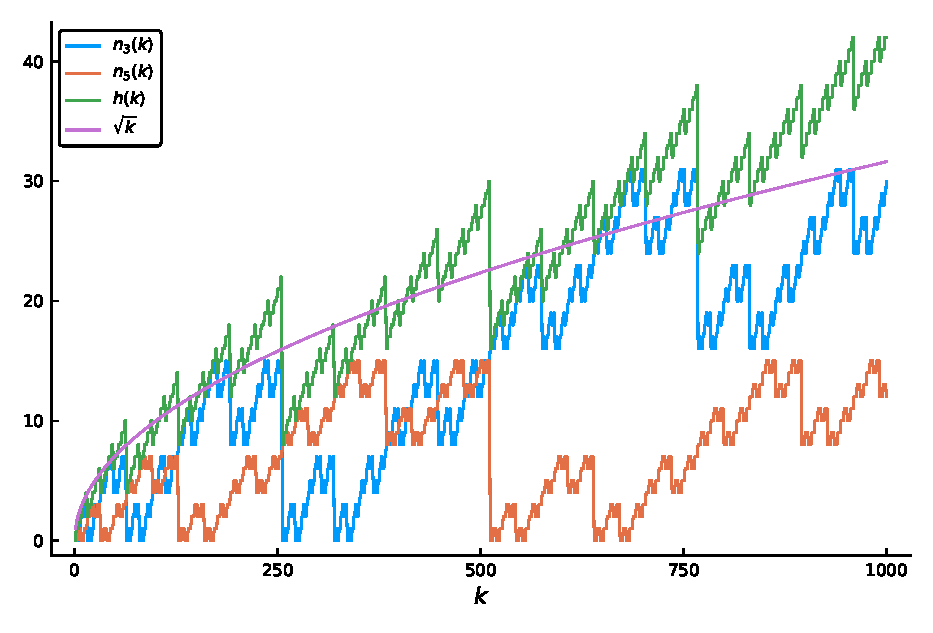
\includegraphics{behaviour_up_to_1000}
	
	(Plot with other scales in \ref{plot:Behaviour_h}.)
\end{center}

\subparagraph{Code's Behaviour}
It may be interesting to represent how the code grows according to both parameters.
First, we can make a small table of values:
\begin{center}
	\begin{tabular}{|c||c|c|c|c|c|c|c|c|c|c|c|}
		\hline
		\textbf{} & \textbf{0} & \textbf{1} & \textbf{2} & \textbf{3} & \textbf{4} & \textbf{5} & \textbf{6} & \textbf{7} & \textbf{8} & \textbf{9} & \textbf{10} \\\hline\hline
		\textbf{0} & 0 & 4 & 16 & 20 & 64 & 68 & 80 & 84 & 256 & 260 & 272 \\
		\textbf{1} & 2 & 6 & 18 & 22 & 66 & 70 & 82 & 86 & 258 & 262 & 274 \\
		\textbf{2} & 8 & 12 & 24 & 28 & 72 & 76 & 88 & 92 & 264 & 268 & 280 \\
		\textbf{3} & 10 & 14 & 26 & 30 & 74 & 78 & 90 & 94 & 266 & 270 & 282 \\
		\textbf{4} & 32 & 36 & 48 & 52 & 96 & 100 & 112 & 116 & 288 & 292 & 304 \\
		\textbf{5} & 34 & 38 & 50 & 54 & 98 & 102 & 114 & 118 & 290 & 294 & 306 \\
		\textbf{6} & 40 & 44 & 56 & 60 & 104 & 108 & 120 & 124 & 296 & 300 & 312 \\
		\textbf{7} & 42 & 46 & 58 & 62 & 106 & 110 & 122 & 126 & 298 & 302 & 314 \\
		\textbf{8} & 128 & 132 & 144 & 148 & 192 & 196 & 208 & 212 & 384 & 388 & 400 \\
		\textbf{9} & 130 & 134 & 146 & 150 & 194 & 198 & 210 & 214 & 386 & 390 & 402 \\
		\textbf{10} & 136 & 140 & 152 & 156 & 200 & 204 & 216 & 220 & 392 & 396 & 408 \\
		\hline
	\end{tabular}

	Table in of (even) integers corresponding to code $[line,column]$.
\end{center}
(Larger table in \ref{table:CodeToIntegers}.)

But it isn't very visual, so another way to view it is as a surface (obtained by linking with triangles the points plotted).
On the grid $\left[ 0,10 \right]^2$, we plot the surface $z = \left[ x, y \right]$ i.e. $z$ is the integer with code $\left[ x, y \right]$.
\begin{center}
	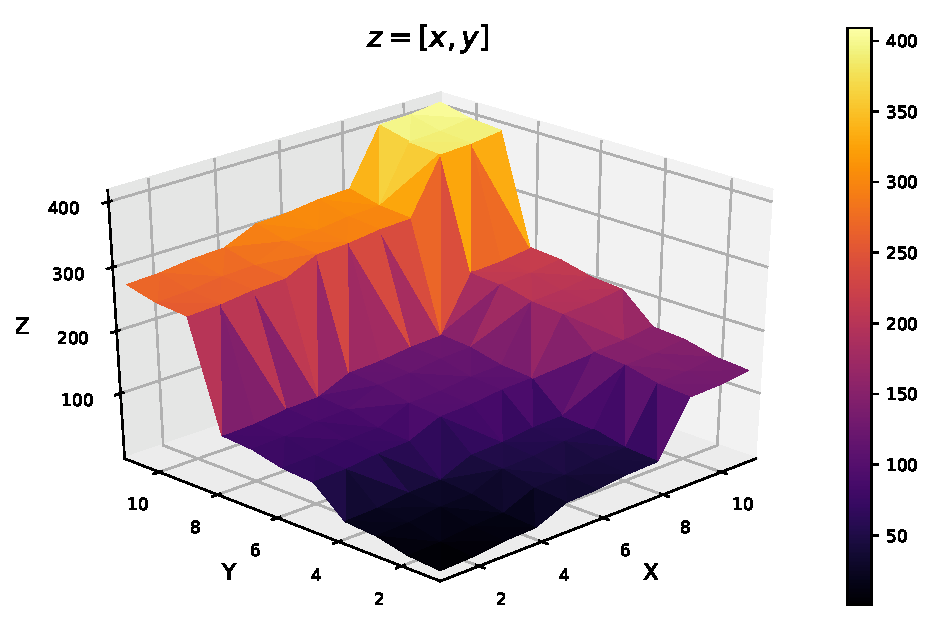
\includegraphics{code_plot_10-10}
	
	Plot of the surface with height given by the code of $X$ and $Y$.\\
	(i.e. the surface with equation $Z = [X,Y]$.)
\end{center}
(Other scales of plots available in \ref{plot:CodeSurface}.)

\paragraph{Order Relation}
We define the following order relation on natural numbers:
For $m, l \in \N$, $m \prec l$ if $h(m) < h(l)$ or $h(m) = h(l)$ and $n_5(m) \prec n_5(l)$.
This relation is a total order, this is straightforward to check.

\subsubsection{Action of $T_3$ and $T_5$}
\paragraph{$h$ on modular forms}
For the rest of the section, we will write a modular form $f \in \mathcal{F}$ as follows:
$f = \Delta^{m_1} + \Delta^{m_2} + \dots + \Delta^{m_r}$ with $m_1 > m_2 > \dots > m_r$.
In this case, $m_1$ is the \textit{degree} of $f$, and we will denote it by $\degree{f}$.
We write $\degree{f} = -\infty$ if $f=0$.
We define $h(f) = h(m_1)$, and $h(f) = -\infty$ if $f=0$.
Similarly, we define $n_3(f) = n_3(m_1)$ and $n_5(f) = n_5(m_1)$, and $n_3(f) = n_5(f) = -\infty$ if $f=0$.

\paragraph{Action of $T_3$}
Here, we want to give a description for the behaviour of $h(T_3|f)$ and $\degree{T_3|f}$.
\label{propositionActionT3}
\begin{proposition}
	Let $f \in \mathcal{F}$ be a non-zero modular form modulo 2.
	\begin{enumerate}
		\item In general, $h(T_3|f) \leq h(f)-1$.
		\item If $n_3(f)>0$, then $h(T_3|f) = h(f)-1$ and $\degree{T_3|f}$ has code $\left[ n_3(f)-1, n_5(f) \right] $.
	\end{enumerate}
\end{proposition}
This proposition is stated in \cite[§4]{OrdreNilpotenceOperateurHecke}, and a complete proof is given in \cite{ModularFormsMcGill}.

\paragraph{Action of $T_5$}
Similarly to the above for $T_3$, we want to give a description for the behaviour of $h(T_5|f)$ and $\degree{T_5|f}$.
\label{propositionActionT5}
\begin{proposition}
	Let $f \in \mathcal{F}$ be a non-zero modular form modulo 2.
	\begin{enumerate}
		\item In general, $h(T_5|f) \leq h(f)-1$.
		\item If $n_5(f)>0$, then $h(T_5|f) = h(f)-1$ and $\degree{T_5|f}$ has code $\left[ n_3(f), n_5(f)-1 \right] $.
	\end{enumerate}
\end{proposition}
Again, this proposition is stated in \cite[§4]{OrdreNilpotenceOperateurHecke}, and a complete proof is given in \cite{ModularFormsMcGill}.



\subsubsection{Formula for the Order of Nilpotency}
\paragraph{Lower bound}
\begin{property}
	Let $f \in \mathcal{F}$ be a non-zero modular form modulo 2 of degree $m_1$.
	Then we have:
	$$
	T_3^{n_3(m_1)} T_5^{n_5(m_1)} | f = \Delta
	$$
\end{property}
\begin{proof}
	We apply $n_3(m_1)$ times the proposition about $T_3$ above, and $n_5(m_1)$ times the proposition about $T_5$, to get that the degree of $g = T_3^{n_3(m_1)}T_5^{n_5(m_1)}|f$ has code $\left[ 0,0 \right]$.
	The propositions also implies that $h(g) > -\infty$, i.e. $g \neq 0$.
	Therefore, $\degree{g} > -\infty$, so it must be odd. since it has code $\left[ 0,0 \right]$,  $\degree{g} = 1$, thus $g = \Delta$.
\end{proof}

\begin{corollary}
	Let $f \in \mathcal{F}$ be a non-zero modular form modulo 2.
	We have $g(f) \geq h(f) +1$.
\end{corollary}
\begin{proof}
	This is directly implied by the proposition:
	As $T_3^{n_3(m_1)}T_5^{n_5(m_1)}|f = \Delta \neq 0$, we have $g(f) \geq n_3(f)+n_5(f)+1 = h(k)+1$.
\end{proof}

\paragraph{Representation of $\mathcal{F}$}
\subparagraph{Table}
This means that for each $k$ odd, there is pair $\left[ a,b \right] = \left[ n_3(k),n_5(k) \right] \in \N\times\N$ (which corresponds to the code of $k$), such that $T_3^aT_5^b|\Delta^k = \Delta$.
Explicitly, $T_3^{n_3(k)}T_5^{n_5(k)}|\Delta^k = \Delta$.
Thus, we can arrange all odd powers of the discriminant $\Delta$ in a table, such that applying the corresponding Hecke operators give exactly $\Delta^1$:
\begin{center}
	\begin{tabular}{|c||ccccccccccc|}
		\hline
		\textbf{} & \textbf{$T_5^{0}$} & \textbf{$T_5^{1}$} & \textbf{$T_5^{2}$} & \textbf{$T_5^{3}$} & \textbf{$T_5^{4}$} & \textbf{$T_5^{5}$} & \textbf{$T_5^{6}$} & \textbf{$T_5^{7}$} & \textbf{$T_5^{8}$} & \textbf{$T_5^{9}$} & \textbf{$T_5^{10}$} \\
		\hline\hline
		$T_3^{0}$ & $\Delta^{1}$ & $\Delta^{5}$ & $\Delta^{17}$ & $\Delta^{21}$ & $\Delta^{65}$ & $\Delta^{69}$ & $\Delta^{81}$ & $\Delta^{85}$ & $\Delta^{257}$ & $\Delta^{261}$ & $\Delta^{273}$ \\
		$T_3^{1}$ & $\Delta^{3}$ & $\Delta^{7}$ & $\Delta^{19}$ & $\Delta^{23}$ & $\Delta^{67}$ & $\Delta^{71}$ & $\Delta^{83}$ & $\Delta^{87}$ & $\Delta^{259}$ & $\Delta^{263}$ & $\Delta^{275}$ \\
		$T_3^{2}$ & $\Delta^{9}$ & $\Delta^{13}$ & $\Delta^{25}$ & $\Delta^{29}$ & $\Delta^{73}$ & $\Delta^{77}$ & $\Delta^{89}$ & $\Delta^{93}$ & $\Delta^{265}$ & $\Delta^{269}$ & $\Delta^{281}$ \\
		$T_3^{3}$ & $\Delta^{11}$ & $\Delta^{15}$ & $\Delta^{27}$ & $\Delta^{31}$ & $\Delta^{75}$ & $\Delta^{79}$ & $\Delta^{91}$ & $\Delta^{95}$ & $\Delta^{267}$ & $\Delta^{271}$ & $\Delta^{283}$ \\
		$T_3^{4}$ & $\Delta^{33}$ & $\Delta^{37}$ & $\Delta^{49}$ & $\Delta^{53}$ & $\Delta^{97}$ & $\Delta^{101}$ & $\Delta^{113}$ & $\Delta^{117}$ 
		& $\Delta^{289}$ & $\Delta^{293}$ & $\Delta^{305}$ \\
		$T_3^{5}$ & $\Delta^{35}$ & $\Delta^{39}$ & $\Delta^{51}$ & $\Delta^{55}$ & $\Delta^{99}$ & $\Delta^{103}$ & $\Delta^{115}$ & $\Delta^{119}$ 
		& $\Delta^{291}$ & $\Delta^{295}$ & $\Delta^{307}$ \\
		$T_3^{6}$ & $\Delta^{41}$ & $\Delta^{45}$ & $\Delta^{57}$ & $\Delta^{61}$ & $\Delta^{105}$ & $\Delta^{109}$ & $\Delta^{121}$ & $\Delta^{125}$ & $\Delta^{297}$ & $\Delta^{301}$ & $\Delta^{313}$ \\
		$T_3^{7}$ & $\Delta^{43}$ & $\Delta^{47}$ & $\Delta^{59}$ & $\Delta^{63}$ & $\Delta^{107}$ & $\Delta^{111}$ & $\Delta^{123}$ & $\Delta^{127}$ & $\Delta^{299}$ & $\Delta^{303}$ & $\Delta^{315}$ \\
		$T_3^{8}$ & $\Delta^{129}$ & $\Delta^{133}$ & $\Delta^{145}$ & $\Delta^{149}$ & $\Delta^{193}$ & $\Delta^{197}$ & $\Delta^{209}$ & $\Delta^{213}$ & $\Delta^{385}$ & $\Delta^{389}$ & $\Delta^{401}$ \\
		$T_3^{9}$ & $\Delta^{131}$ & $\Delta^{135}$ & $\Delta^{147}$ & $\Delta^{151}$ & $\Delta^{195}$ & $\Delta^{199}$ & $\Delta^{211}$ & $\Delta^{215}$ & $\Delta^{387}$ & $\Delta^{391}$ & $\Delta^{403}$ \\
		$T_3^{10}$ & $\Delta^{137}$ & $\Delta^{141}$ & $\Delta^{153}$ & $\Delta^{157}$ & $\Delta^{201}$ & $\Delta^{205}$ & $\Delta^{217}$ & $\Delta^{221}$ & $\Delta^{393}$ & $\Delta^{397}$ & $\Delta^{409}$ \\
		\hline
	\end{tabular}

	Table of powers $\Delta^k$ such that the corresponding operator applied to $\Delta^k$ gives $\Delta^1$.\\
	(i.e. $\Delta^k$ such that $T_3^{line}T_5^{column}|\Delta^k = \Delta$.)
\end{center}
(A larger table can be found in \ref{table:OperatorToDelta1}.)

From the fact that codes are in bijection with odd integers, we can use this table as a basis for modular forms modulo 2.


\paragraph{Exact Formula}
We derive here an explicit formula for the order of nilpotency of a modular form modulo 2.
\label{theoremOrderOfNilpotency}
\begin{theorem}[Order of Nilpotency of Modular Forms Modulo 2] \cite[§5]{OrdreNilpotenceOperateurHecke}.
	Let $f \in \mathcal{F}$ be a non-zero modular form modulo 2.
	The order of nilpotency is exactly $g(f) = h(f) + 1$.
\end{theorem}
What remains to prove is that $g(f) \leq h(f) + 1$.
This is proved in \cite[§5]{OrdreNilpotenceOperateurHecke}.

From this follows a new remark, which is useful to estimate computations times:
As $g(f)=h(f)+1$, and $h(f) = h(\degree{f}) = \mathcal{O}(\sqrt{\degree{f}})$, we have $g(f) = \mathcal{O}(\sqrt{\degree{f}})$, i.e. the nilpotency order of a modular form behaves asymptotically as the square root of its degree.

\label{corollaryOrderOfNilpotency}
\begin{corollary}
	Let $f \in \mathcal{F}$ be a non-zero modular form modulo 2.
	If $T_3|f = T_5|f = 0$, then $f = \Delta$.
\end{corollary}
\begin{proof}
	By the previous proposition, we have both $n_3(f)=0$ and $n_5(f)=0$.
	Thus, $\degree{f}$ has code $\left[ 0,0 \right]$.
	Since $f \neq 0$ and $f \in \mathcal{F}$, this means $f = \Delta$.
\end{proof}

	% !TeX spellcheck = en_GB
\section{Hecke Algebra}
This section follows from \cite{StructureAlgebreHecke}.

We recall $\mathcal{F} = \left\langle \Delta^k \ | \ k \text{ odd} \right\rangle$, i.e. $\mathcal{F} = \left\langle \Delta, \Delta^3, \Delta^5, \Delta^7, \Delta^9, \dots \right\rangle$
\subsection{Definition}
We redefine $ \mathcal{F}(n) = \left\langle \Delta, \Delta^3, \Delta^5, \dots, \Delta^{2n-1} \right\rangle $ so that $\dim(\mathcal{F}(n)) = n$

We define $A(n)$ as the $\F_2$-subalgebra of $\End{\mathcal{F}(n)}$ given by $\F_2$ and $T_p$. That is, if 
$
\mathfrak{m}(n) = \{T_{p_1} \cdot T_{p_2} \cdots T_{p_k} | p_1, p_2, \dots, p_k \in \primes, k\geq 1\}
$
is a sub-vector-space of $\mathcal{F}$, we get $A(n) = \F_2 \oplus \mathfrak{m}(n)$.

\begin{property}
	$\mathfrak{m}(n)$ is the only maximum ideal of $A(n)$.
\end{property}
\begin{proof}
	Firstly, we note that $\nicefrac{A(n)}{\mathfrak{m}} \cong \F_2$.
	Since $\F_2$ is a field, $\mathfrak{m}$ must be a maximum ideal.
	
	Now, suppose $I$ is an other (i.e. $I \neq \mathfrak{m}$) maximum ideal of $A(n)$.
	Then there is an operator $u \in \mathfrak{m}$ such that $(1+u) \in I$.
	Since Hecke operators are nilpotent \ref{NilpotencyHeckeOperators}, there exists $n \in \N$ such that $u^n=0$.
	By induction, $(1+u^n) \in I$ for all $n \geq 1$.
	% Suppose $(1+u^n) \in I$. As $(1+u) \in I$ we then get $(1+u)(1+u^n)+(1+u)+(1+u^n) = 1+u+u^n+u^{n+1}+1+u+1+u^n = 1+u^{n+1}] \in I$
\end{proof}

Note that as Hecke operators are all nilpotent \ref{NilpotencyHeckeOperators}, the ideal $\mathfrak{m}(n)$ is itself nilpotent.
In fact, from the minimum \ref{MinimumOrderNilpotencyHeckeOperators} and maximum \ref{MaximumOrderNilpotencyHeckeOperators} nil-potency order property extend to the ideal $\mathfrak{m}$.

Let the dual of $\mathbb{F}(n)$ be $\mathcal{F}(n)^* = \{ F: \mathcal{F} \to \F_2 \}$.
Then $\mathbb{F}(n)^*$ is an $A(n)$-module with operation 
$ (u \cdot F)(f) = F(u | f) $ for $u \in A(n)$ and $F \in \mathcal{F}(n)$.

We define $e_n$ to be the element of $\mathcal{F}(n)$ such that $e_n(\Delta) = 1$ and $e_n(\Delta^{2j+1}) = 0$ for all $1 \leq j <n$ (i.e. characteristic of $\Delta$).\\
Denote the $q$-coefficients of a modular form $f$ by $a_m(f)$, so $f = \sum_{m>0} a_m(f)q^m$.
Then $e_n(f) = a_1(f)$.
For an odd prime $p$, have $a_1(T_p|f) = a_p(f)$, so $T_p \cdot e_n(f) = a_p(f)$.
By induction, this gives for odd primes $p_1, p_2, \dots, p_k$:
$$
T_{p_1} T_{p_2} \cdots T_{p_k} \cdot e_n(f) 
= a_{p_1 p_2\cdots p_k}(f)
$$

\subsection{Basic Properties}

\begin{property}
	Note that for a non zero modular forms $f \in \mathcal{F}(n)$, there exists an operator $u \in A(n)$ such that $e_n(u|f) = 1$.
\end{property}
\begin{proof}
	We can write $f = q^m + \mathcal{O}(q^{m+1})$ for some $m$ odd (as $\mathcal{F}(n)$ is generated by odd powers of $\Delta$).
	Now, as $m$ is odd, $m=p_1 p_2 \cdots p_k$ with $p_i$ odd primes for all $1 \leq i \leq k$.
	Then, by the above, $T_{p_1} T_{p_2} \cdots T_{p_k} \cdot e_n(f) = a_m(f) = 1$.
	Letting $u = T_{p_1} T_{p_2} \cdots T_{p_k}$, we have $e_n(u|f) = u \cdot e_n(f) = 1$.
\end{proof}

\begin{property}
	$\mathcal{F}(n)^*$ is free as an $A(n)$-module, with basis $e_n$;	
	i.e., $\mathcal{F}(n)^* = A(n) \cdot e_n$.
\end{property}
\begin{proof}
	By contradiction, suppose $(e_n)$ (the $A(n)$-module generated by $e_n$) isn't $\mathcal{F}(n)^*$.
	The there must be a non-zero modular form $f \in \mathcal{F}(n)$ such that $u \cdot e_n(f)=0$ for all $u \in A(n)$.
	This would contradict the last property.
	Therefore, we have $\mathcal{F}(n)^* = A(n) \cdot e_n$.
\end{proof}

\begin{corollary}
	From last property, we deduce:
	\begin{itemize}
		\item The map $\phi: A(n) \to \mathcal{F}(n)^*$ such that $\phi(u) = u \cdot e_n$ is a bijection.
		\item The dimension of $A(n)$ is $n$.
		\item There is a bijection $\phi: A(n) \to \mathcal{F}(n)^*$.
	\end{itemize}
\end{corollary}
\begin{proof}
	We prove separately:
	\begin{itemize}
		\item This follows directly from the fact that $\mathcal{F}(n)^* = A(n) \cdot e_n$.
		\item We have $\dim(A(n)) = \dim(\mathcal{F}(n)^*)$ by the above, and $\dim(\mathcal{F}(n)^*) = \dim(\mathcal{F}(n))$ by duality.
		\item Since $\mathcal{F}(n)^* \leftrightarrow A(n)$
		\footnote{$A \leftrightarrow B$ means there exists a bijection from $A$ to $B$}, $\mathcal{F}(n)^{**} \leftrightarrow A(n)^*$.
		And as $\mathcal{F}(n)^{**} \cong \mathcal{F}(n)$, we have $\mathcal{F}(n) \leftrightarrow A(n)^*$.
	\end{itemize}
\end{proof}


\subsection{Generated by $T_3$ and $T_5$}







	% !TeX spellcheck = en_GB
\section{Frobenian Elements}
\subsection{Context}
\subsubsection{General}
\paragraph{Basic Properties}
Let $R$ be a commutative ring, $M$ and $P$ ideals in $R$.
We can then prove the followings:
\begin{itemize}
    \item $M \text{ is maximal} \iff R/M \text{ is a field}$
    \item $P \text{ is prime} \iff R/P \text{ is an integral domain}$
\end{itemize}

Moreover, we have:
\begin{property}
    Maximal ideals are prime. 
\end{property}
\begin{proof}
    \begin{align*}
        M \text{ maximal ideal} &\iff R/M \text{ field}\\
                                &\implies \text{ R/M Integral Domain } \iff M \text{ prime ideal}
    \end{align*}
\end{proof}

\paragraph{Definitions and Notations}
If $L/K$ is a Galois extension, then we will denote it's Galois group by $\Gal{L/K}$.

Let $K$ be a number field, and $\mathcal{O}_K$ be the corresponding ring of integers.
Let $\mathfrak{p}$ be a non-zero prime ideal in $\mathcal{O}_K$.
Let $L/K$ be a finite extension and again, $\mathcal{O}_L$ be the ring of integers in $L$.
Then we know that $\mathcal{O}_L$ is the integral closure of $\mathcal{O}_K$ in $L$
We have $\mathfrak{p}\mathcal{O}_L$ an ideal in $\mathcal{O}_L$.
It is not a prime ideal in general, but as $L/K$ is finite, there exists a factorization as the following:
$$
\mathfrak{p}\mathcal{O}_L = \prod_{i=1}^r \mathfrak{P}_i^{e_i}.
$$
Where the integers $e_i$ are called the ramification indexes.
We also have $\mathfrak{P}_i \cap \mathcal{O}_K = \mathfrak{p}$, and we say that the ideals $\mathfrak{P}_i$ in $L$ extend the ideal $\mathfrak{p}$ in $K$.

Then, there are three possibilities for an ideal: it may split, ramify of be inert.
\begin{definition}[Ideal Ramifies]
    We say that an ideal $\mathfrak{p}$ ramifies in $L/K$ if a ramification index $e_i$ is greater then one, 
    i.e. if $e_i>1$ for some $1 \leq i \leq r$.
\end{definition}
\begin{definition}[Ideal Splits]
    We say that $\mathfrak{p}$ splits in $L/K$ if none of the ramification indexes $e_i$ is greater then one, and $r$ is a least two; 
    i.e. if $e_i=1 \quad \forall 1 \leq i \leq r$ and $r \geq 2$.
\end{definition}
\begin{definition}[Ideal Inert]
    We say that $\mathfrak{p}$ is inert in $L/K$ if there is only one ramification index $e_1$ and it is equal to one;
    i.e. if $e_1=1$ and $r=1$.
\end{definition}
We know that the extension $L/K$ is ramified in the primes that divide the discriminant. Therefore, the extension is unramified in all but finitely many prime ideals.


\subsubsection{Residue Fields Extensions}
The ideal $\mathfrak{p}$ defines the \textit{residue field} $F=\mathcal{O}_K/\mathfrak{p}$.
The ideals $\mathfrak{P}_i$ define the \textit{residue fields} $F_i=\mathcal{O}_L/\mathfrak{P}_i$.\\
The field $F$ then naturally embeds to $F_i$ (so each $\mathfrak{P}_i$ defines a field extension).
The \textit{inertia degree} of $\mathfrak{P}_i$ is the degree $f_i=[F_i:F]=[\mathcal{O}_L/\mathfrak{P}_i:\mathcal{O}_K/\mathfrak{p}]$ of this extension.
We then observe that $[L:K] = \sum_{i=1}^r e_if_i$
We can then specify when an ideal splits or ramifies completely:
\begin{definition}[Ideal Splits Completely]
    We say that $\mathfrak{p}$ splits completely in $L/K$ if all ramification indexes $e_i$ and inertia degrees $f_i$ are one.
    i.e. if $e_i=f_i=1 \quad \forall 1 \leq i \leq r$.\\
    In this case, $r=[L:K]$.
\end{definition}
\begin{definition}[Ideal Ramifies Completely]
    We say that $\mathfrak{p}$ ramifies completely in $L/K$ if the inertia degrees $f_1$ is one, and $r$ is one.
    i.e. if $r=1$ and $f_1=1$.\\
    In this case, $e_1=[L:K]$.
\end{definition}

\subsubsection{Norms of Ideals}
We define the \textit{norm of an ideal} $I$ in $\mathcal{O}_K$ as $N(I)=|\mathcal{O}_K/I|$.
If $\mathfrak{p} \subset \mathcal{O}_K$ is a prime ideal, then we can put $(p)=\mathfrak{p} \cap \Z$.
It follows that $p\mathcal{O}_K \subset \mathfrak{p}$.
$\mathcal{O}_K$ is a free $\Z-module$ of rank $[K:\Q]=q$, i.e. $\exists \alpha_1,\dots,\alpha_q \text{ s.t. } \mathcal{O}_K=\Z \alpha_1 \oplus \cdots \oplus \Z \alpha_q$.
Thus, $|\mathcal{O}_K/\mathfrak{p}| \leq |\mathcal{O}_K/(p)| \leq p^q$.
We have $\Norm{\mathfrak{p}} = |\mathcal{O}_K/\mathfrak{p}|=p^m$ and $\Norm[L/\Q]{\mathfrak{P}_i} = \Norm[K/\Q]{\mathfrak{p}}^{f_i}$.
This implies $\Norm{\mathfrak{P}_i} = |\mathcal{O}_L/\mathfrak{P}_i| = p^{mf_i}$.\\
We also have: 
$\mathcal{O}_K/\mathfrak{p} \cong \mathbb{F}_{\Norm{\mathfrak{p}}}$ and $\mathcal{O}_L/\mathfrak{P}_i \cong \mathbb{F}_{\Norm{\mathfrak{P}_i}}$.

\subsubsection{Galois Extension Simplifications}
When the extension $L/K$ is Galois, the ramification indexes $e_i$ are all the same ($e_i=e$), as well as the inertia degrees $f_i=f$.
We then have
$$
\mathfrak{p}\mathcal{O}_L = \prod_{i=1}^r \mathfrak{P}_i^{e}
\text{ and } [L:K] = ref.
$$
The Galois group $\Gal{L/K}$ is often denoted $G$.

We define the \textit{decomposition group} $G_{\mathfrak{P}}$ of the ideal $\mathfrak{P}$ to be $\{\sigma \in G \mid \sigma(\mathfrak{P})=\mathfrak{P} \}$.
It turns out that 
$G_{\mathfrak{P}} 
\cong \Gal{\nicefrac{\mathcal{O}_L/\mathfrak{P}}{\mathcal{O}_K/\mathfrak{p}}}
\cong \Gal{ \mathbb{F}_{p^{mf}}/\mathbb{F}_{p^{f}}}$.
Moreover, it is a cyclic group, so $G_{\mathfrak{P}} = <\tilde{\sigma}>$.

\subsubsection{Unramified Prime Simplifications}
When the ideal $\mathfrak{p}$ is unramified, $e=1$, so we get:
$$
\mathfrak{p}\mathcal{O}_L 
= \prod_{i=1}^r \mathfrak{P} \text{ and } [L:K] = rf.
$$

\subsection{The Frobenius Element}
\subsubsection{Definition}
We can construct the \textit{Frobenius element} (sometimes also called the \textit{Artin symbol}, or the \textit{Frobenius map}) that depend on the extension $L/K$ and ideal $\mathfrak{P}$ in $\mathcal{O}_L$.
It is denoted $\Frob{L/K}{\mathfrak{P}}$, and is \textit{the} element $\sigma \in G$ such that:
$$
\sigma \mathfrak{P} = \mathfrak{P}
\quad \text{ and } \quad
\sigma(\alpha) \equiv \alpha^{\Norm[K/\Q]{\mathfrak{p}}} \bmod{\mathfrak{P}} \quad \forall \alpha \in \mathcal{O}_L.
$$

The second condition is the interesting one; while the first is only useful to make the Frobenius element unique.
The second condition defines a unique element only up to conjugacy class.
Most of the time, we will consider abelian extensions, so the conjugacy classes will only have one element, and the first condition will be dropped.

We define the \textit{Frobenius element} for $\mathfrak{p}$ (denoted $\Frob{L/K}{\mathfrak{p}}$) in a meaning full manner, to be the set
$$
\{\Frob{L/K}{\mathfrak{P}} | \mathfrak{P} \text{ extending } \mathfrak{p}\} \subset G
.$$

The following properties imply that $\Frob{L/K}{\mathfrak{p}}$ is in fact a conjugacy class in the Galois group $\Gal{L/K}$.
Hence, we refer to $\Frob{L/K}{\mathfrak{p}}$ as the Frobenius conjugacy class.

\begin{property}
	If $\tau \in G$, then 
	$\Frob{L/K}{\mathfrak{\tau P}} = \tau \Frob{L/K}{\mathfrak{P}} \tau^{-1}$.
\end{property}
\begin{proof}
	For all $x \in \mathcal{O}_L$, we have:
	$$
	\Frob{L/K}{\mathfrak{P}}x 
	= x^{\Norm[K/\Q]{\mathfrak{p}}} \mod \mathfrak{P}
	$$
	But all such $x$ may be written as $\tau^{-1}(x)$, so we have:
	$$
	\Frob{L/K}{\mathfrak{P}} \tau^{-1}(x) 
	= {(\tau^{-1} x)}^{\Norm[K/\Q]{\mathfrak{p}}} \mod \mathfrak{P}.
	$$
	Which gives:
	$$
	\tau \Frob{L/K}{\mathfrak{P}}\tau^{-1}(x) 
	= x^{\Norm[K/\Q]{\mathfrak{p}}} \mod \mathfrak{P}.
	$$
\end{proof}


\begin{property}
	If $\mathfrak{P}_1$ and $\mathfrak{P}_2$ extend $\mathfrak{p}$, then $\Frob{L/K}{\mathfrak{P}_1}$ and $\Frob{L/K}{\mathfrak{P}_2}$ are conjugates.
\end{property}
\begin{proof}
	We have the following scheme:\\
	\begin{tikzpicture}[text width=10cm, align=flush center]
	%nodes
	\node (L)                                           {$L$};
	
	\node (subsetL)[right of=L, node distance=0.75cm]   {$\supseteq$};
	\node (P1)[right of=subsetL, node distance=0.75cm]  {$\mathfrak{P}_1$};
	\node (P2)[right of=P1, node distance=1cm]          {$\mathfrak{P}_2$};
	
	\node (K) [below of=L, node distance=2cm]           {$K$};
	\node (subsetK)[right of=K, node distance=1cm]      {$\supseteq$};
	\node (p) [right of=subsetK, node distance=1cm]     {$\mathfrak{p}$};
	
	%links
	\draw[-] (L) to node {} (K);
	\draw[-] (p) to node {} (P1);
	\draw[-] (p) to node {} (P2);
	\end{tikzpicture}
	
	There is an element $\tau \in G$ such that $\tau(\mathfrak{P}_1)=\mathfrak{P}_2$.
	Then using last property, we deduce that $\Frob{L/K}{\mathfrak{P}_1}$ and $\Frob{L/K}{\mathfrak{P}_2}$ are conjugates.
\end{proof}

Never the less, is important to notice at this point that if $L/K$ is an abelian extension (i.e. $G$ is abelian), then every conjugacy class in $\Gal{L/K}$ is made up of only one element.
In this case, we sometimes use $\Frob{L/K}{\mathfrak{p}}$ to denote the Frobenius element $\Frob{L/K}{\mathfrak{P}}$, where $\mathfrak{P}$ is any prime lying above $\mathfrak{p}$.



\subsubsection{Examples}
\paragraph{$\Q[\sqrt{7}]/\Q$ (quadratic field extension)}
\label{QuadraticExtensionExample}
%Looking at $\Q[\sqrt{7}]:\Q$ (which is a Galois extension).
We have minimum polynomial $m(x)=x^2-7$, the discriminant is $\Delta = 4.7 = 28$.\\
We write
$$
G = \Gal{\Q[\sqrt{7}]:\Q} = <\sigma \mid \sigma^2 = 1_G> \cong C_2.
$$
As $C_2$ is abelian, we will have no problem defining Frobenius elements.

\subparagraph{The prime ideal $(3)$}
%We look at the prime ideal $(3)$:
As $m(x) = (x+1)(x-1) \mod 3$, we have $(3) = (3, \sqrt{7}+1)(3, \sqrt{7}-1)$.\\
As well, $\Norm[{\Q[\sqrt{7}]/\Q}]{(3)} = 3$ and $\Norm[{\Q[\sqrt{7}]/\Q}]{(3, \sqrt{7}+1)} 
=\Norm[{\Q[\sqrt{7}]/\Q}]{(3, \sqrt{7}-1)} 
= 3
$, but $\Norm[\Q/\Q]{(3)} = 3$.
So we have:
\begin{align*}
    \Frob{\Q[\sqrt{7}]:\Q}{(3, \sqrt{7}+1)}:
    \alpha   &\mapsto \alpha^{\Norm[\Q/\Q]{(3)}} \bmod (3, \sqrt{7}+1)\\
    \sqrt{7} &\mapsto \left( \sqrt{7} \right)^3 \equiv \sqrt{7} \bmod (3, \sqrt{7}+1)
\end{align*}
Thus, $\Frob{\Q[\sqrt{7}]:\Q}{(3, \sqrt{7}+1)} = 1_G \in G$.
Similarly, $\Frob{\Q[\sqrt{7}]:\Q}{(3, \sqrt{7}-1)} = 1_G \in G$.

\subparagraph{The prime ideal $(5)$}
%We look at the prime ideal $(5)$:
As $m(x)$ has no root $\bmod 2$. So $m(x)$ is irreducible $\bmod 5$ and $(5)$ is inert in $\Q[\sqrt{7}]$
As well, $\Norm[{\Q[\sqrt{7}]/\Q}]{(5)} = 5^2 = 25$ but $\Norm[\Q/\Q]{(5)} = 5$.
So we have:
\begin{align*}
    \Frob{\Q[\sqrt{7}]:\Q}{(5)}: 
    \alpha   &\mapsto \alpha^{\Norm[\Q/\Q]{(5)}} \bmod (5)\\
    \sqrt{7} &\mapsto \left( \sqrt{7} \right)^5 \equiv -\sqrt{7} \bmod (5)
\end{align*}
Thus, $\Frob{\Q[\sqrt{7}]:\Q}{(5)} = \sigma \in G$.

\paragraph{$\Q[\zeta_n]/\Q$ ($n^{th}$ Cyclotomic Field Extensions)}
We have minimum polynomial:
$$
\Phi(x)= \prod_{\substack{1 \leq k \leq n \\ \gcd(k,n)=1}} 
\left( x-e^{2 i \pi \frac{k}{n}} \right)
$$
(so degree of the extension is $\varphi(n)$, where $\varphi$ is Euler totient function).
Discriminant of the extension is:
$$
\Delta = (-1)^{\varphi(n)/2}
\frac{n^{\varphi(n)}}{\prod_{p \mid n} p^{\varphi(n)/(p-1)}};
$$
see \cite[Proposition 2.7]{IntroductionToCyclotomicFields}.

The Galois group $G$ consist of $\sigma_k$ such that $\sigma_k(\zeta_n^i)=\zeta_n^{ik}$, with $\gcd(k,n)=1$.)
Note as well that $G$ is abelian, so it is simple to calculate the Frobenius element.
It is straightforward that $G$ is naturally isomorphic to the multiplicative group $\left( \nicefrac{\Z}{n\Z} \right)^\times$.
Note that $\sigma \in G$ is determined by $\sigma(\zeta_n)$.
Note as well that this group is abelian.

With $p \in \primes$, a prime that is unramified in $\Q[\zeta_n]/\Q$, let $P$ be an ideal lying above $(p)$.
We want to look at $\Frob{\Q[\zeta_n]/\Q}{P}$.
We have:
\begin{align*}
	\Frob{\Q[\zeta_n]/\Q}{P}: 
	\alpha&\mapsto \alpha^{\Norm[\Q/\Q]{(p)}} \bmod P\\
	\zeta_n&\mapsto \zeta_n^p \bmod P
\end{align*}

\paragraph{Case $\Q[\zeta_{10}]/\Q$ ($10^{th}$ cyclotomic field extension)}
We denote by $\zeta_{10}=e^{\pi i/5}$ the $10^{th}$ root of unity.
We have minimum polynomial $m(x) = x^4-x^3+x^2-x+1$ (so degree of the extension is 4), the discriminant is $\Delta = 5^3$.

We write $
G = \Gal{\Q[\zeta_{10}]:\Q} 
= < \sigma: \zeta_{10} \mapsto \zeta_{10}^3 \mid \sigma^4 = Id > \cong C_4$.

%\begin{center}
%	\begin{tabular}{r|l}
%		$x$ & $x^4-x^3+x^2-x+1$ \\
%		\hline
%		$-5$ & $781 = 11 \cdot 71$ \\
%		$-4$ & $341 = 11 \cdot 31$\\
%		$-3$ & $121 = 11^2$\\
%		$-2$ & $31$\\
%		$-1$ & $5$\\
%		$0$  & $1$\\
%		$1$  & $1$\\
%		$2$  & $11$\\
%		$3$  & $61$\\
%		$4$  & $205 = 5 \cdot 41$\\
%		$5$  & $521$\\		
%	\end{tabular}
%\end{center}



\subparagraph{The prime ideal $(3)$}
%We look at the prime ideal $(3)$:
As $m(x)$ has no root $\bmod 3$, so $(3)$ is inert.
We have:
\begin{align*}
	\Frob{\Q[\zeta_{10}]/\Q}{(3)}:
	\alpha   &\mapsto \alpha^{\Norm[\Q/\Q]{(3)}} \bmod (3)\\
	\zeta_{10} &\mapsto \left( \zeta_{10} \right)^3 \bmod (3)
\end{align*}
Thus, $\Frob{\Q[\zeta_{10}]:\Q}{(3)} = \sigma \in G$.

\subparagraph{The prime ideal $(7)$}
%We look at the prime ideal $(3)$:
As $m(x)$ has no root $\bmod 7$, so $(7)$ is inert.
We have:
\begin{align*}
	\Frob{\Q[\zeta_{10}]/\Q}{(7)}:
	\alpha   &\mapsto \alpha^{\Norm[\Q/\Q]{(7)}} \bmod (7)\\
	\zeta_{10} &\mapsto \left( \zeta_{10} \right)^7 \bmod (7)
\end{align*}
Thus, $\Frob{\Q[\zeta_{10}]:\Q}{(7)} = \sigma^3 \in G$.

\subparagraph{The prime ideal $(11)$}
As $m(x) = (x-2)(x+3)(x+4)(x+4) \bmod 11$, so $(11)$ splits.
We have:
\begin{align*}
	\Frob{\Q[\zeta_{10}]/\Q}{(11)}:
	\alpha   &\mapsto \alpha^{\Norm[\Q/\Q]{(11)}} \bmod (11)\\
	\zeta_{10} &\mapsto \left( \zeta_{10} \right)^{11} = \zeta_{10} \bmod (11)
\end{align*}
Thus, $\Frob{\Q[\zeta_{10}]:\Q}{(11)} = \sigma^4 = Id \in G$.



\subsubsection{Behaviour in Towers of Fields}
We will consider the following scheme:\\
\begin{tikzpicture}[text width=10cm, align=flush center, node distance=0.75cm]
%nodes

\node (M)                                      {$M$};
\node (subsetM)[left of=M, node distance=0.5cm]  {$\subset$};
\node (OM)[left of=subsetM, node distance=0.5cm] {$\mathcal{O}_M$};
\node (supsetM)[right of=M]                    {$\supseteq$};
\node (PM)[right of=supsetM]                   {$\mathfrak{P}$};


\node (L) [below of=M, node distance=2cm]      {$L$};
\node (subsetL)[left of=L, node distance=0.5cm]  {$\subset$};
\node (OL)[left of=subsetL, node distance=0.5cm] {$\mathcal{O}_L$};
\node (supsetL)[right of=L]                    {$\supseteq$};
\node (PL)[right of=supsetL]                    {$\mathfrak{p}$};


\node (K) [below of=L, node distance=2cm]        {$K$};
\node (subsetK)[left of=K, node distance=0.5cm]  {$\subset$};
\node (OK)[left of=subsetK, node distance=0.5cm] {$\mathcal{O}_K$};
\node (supsetK)[right of=K]                    {$\supseteq$};
\node (PK)[right of=supsetK]                    {$p$};


%links
\draw[-] (M) to node {} (L);
\draw[-] (L) to node {} (K);
\draw[-] (PM) to node {} (PL);
\draw[-] (PL) to node {} (PK);
\end{tikzpicture}

In such a situation, we can define (for $M/K$ Galois)
$\Frob{M/K}{\mathfrak{P}}$, 
$\Frob{M/K}{p}$, 
$\Frob{M/L}{\mathfrak{P}}$, 
$\Frob{M/L}{\mathfrak{p}}$.
If, in addition, $L/K$ is normal, we can as well define:
$\Frob{L/K}{\mathfrak{p}}$ , and 
$\Frob{L/K}{p}$ (see \cite[p.99]{AlgebraicNumberFields}).
We will look at properties of these Frobenius elements (relation between each others).

\begin{property}\cite[p.99]{AlgebraicNumberFields}:
	We have 
	$$
	\Frob{M/K}{\mathfrak{P}}^{f(\mathfrak{P}/\mathfrak{p})} = \Frob{M/L}{\mathfrak{P}}.
	$$
\end{property}

\begin{property}
	$$
	\Frob{L/K}{\mathfrak{p}} = \left. \Frob{M/K}{\mathfrak{P}} \right|_L
	$$
\end{property}
\begin{proof}
	Let $\sigma = \Frob{M/K}{\mathfrak{P}} \in \Gal{M/K}$ so 
	$\sigma: M \to M \text{ s.t. } \left. \sigma \right|_K = Id \text{ and } \sigma \text{ is an autotomorphism}$.\\
	Similarly, let $\tau = \Frob{L/K}{\mathfrak{p}} \in \Gal{L/K}$ so 
	$\tau: L \to L \text{ s.t. } \left. \tau \right|_K = Id \text{ and } \tau \text{ is an autotomorphism}$.
	
	As $M$ extends $L$, $\sigma$ being an automorphism of $M$ makes it an automorphism of $L$ as well.
	The restriction condition stays the same.
	% done with Djordjo
	% \cite[p.99]{AlgebraicNumberFields}
\end{proof}


\begin{property}
	$$
	\Gal{L/K} \cong \nicefrac{\Gal{M/K}}{\Gal{M/L}}
	$$
\end{property}
\begin{proof}
	Let $\sigma \in \Gal{M/K}$, i.e. $\sigma: M \to M \text{ s.t. } \left. \sigma \right|_K = Id \text{ and } \sigma \text{ is an autotomorphism}$.
	
	Let $\phi: \Gal{M/K} \to \Gal{L/K}$ be such that:
	$\phi(\sigma) = \left. \sigma \right|_L$.
	This is well defined as an automorphism of $M$ restricts to an automorphism of $L$ when $M$ extends $L$.
	
	It is trivial to check that $\phi$ is a homomorphism.
	
	The kernel of $\phi$ is clearly $\Gal{M/L}$.
	
	The image of $\phi$ is $\Gal{L/K}$ as every element of $\Gal{L/K}$ may be extended to $\Gal{M/K}$.
	
	Therefore, the property follows via the $1^{st}$ isomorphism theorem.
	% done with Djordjo
\end{proof}

\begin{property}\cite[p.100]{AlgebraicNumberFields}:
	We have
	$$
	\mathfrak{p} \text{ splits complitely in } L 
	\iff \Frob{L/K}{\mathfrak{P}} = 1.
	$$
\end{property}

We will consider the following scheme:\\
\begin{tikzpicture}[text width=10cm, align=flush center, node distance=2cm]
%nodes
\node (M) {$L_1L_2$};
\node (supsetM)[right of=M, node distance=0.75cm] {$\supseteq$};
\node (PM)[right of=supsetM, node distance=0.5cm] {$\mathfrak{P}$};

\node (L1) [below of=M, left of=M] {$L_1$};
\node (supsetL1)[right of=L1, node distance=0.5cm] {$\supseteq$};
\node (PL1)[right of=supsetL1, node distance=0.5cm] {$\mathfrak{p}_1$};

\node (L2) [below of=M, right of=M] {$L_2$};
\node (supsetL2)[right of=L2, node distance=0.5cm] {$\supseteq$};
\node (PL2)[right of=supsetL2, node distance=0.5cm] {$\mathfrak{p}_2$};

\node (K) [below of=M, node distance = 4cm] {$K$};
\node (supsetK)[right of=K, node distance=0.5cm] {$\supseteq$};
\node (PK)[right of=supsetK, node distance=0.5cm] {$\mathfrak{p}$};


%links
\draw[-] (M) to node {} (L1);
\draw[-] (M) to node {} (L2);
\draw[-] (L1) to node {} (K);
\draw[-] (L2) to node {} (K);
\end{tikzpicture}



\begin{property}\cite[p.100]{AlgebraicNumberFields}:
	We have
	$$
	\Frob{L_1L_2/K}{\mathfrak{P}}
	= \Frob{L_1/K}{\mathfrak{p}_1} \times \Frob{L_2/K}{\mathfrak{p}_2}.
	$$
\end{property}


\begin{property}\cite[p.100]{AlgebraicNumberFields}:
	We have
	$$
	\mathfrak{p} \text{ splits complitely in } L_1L_2
	\iff
	\mathfrak{p} \text{ splits complitely in } L_1 \text{ and } L_2.
	$$
\end{property}
\begin{proof}
	Combine the last two proposition.
\end{proof}





\subsection{The Chebotarev's Density Theorem}
\subsubsection{Motivations}
\label{DensityMotivation}
If we look at the distribution of primes numbers modulo a number (15 in the next example), we get a table as follows:

Table mod 15:
\begin{center}
	\begin{tabular}{r|l}
		$\bmod 15$ & primes (up to 500)\\
		\hline
		0& \\
		1& 31, 61, 151, 181, 211, 241, 271, 331, 421, \\
		2& 2, 17, 47, 107, 137, 167, 197, 227, 257, 317, 347, 467, \\
		3& 3, \\
		4& 19, 79, 109, 139, 199, 229, 349, 379, 409, 439, 499, \\
		5& 5, \\
		6& \\
		7& 7, 37, 67, 97, 127, 157, 277, 307, 337, 367, 397, 457, 487, \\
		8& 23, 53, 83, 113, 173, 233, 263, 293, 353, 383, 443, \\
		9& \\
		10& \\
		11& 11, 41, 71, 101, 131, 191, 251, 281, 311, 401, 431, 461, 491, \\
		12& \\
		13& 13, 43, 73, 103, 163, 193, 223, 283, 313, 373, 433, 463, \\
		14& 29, 59, 89, 149, 179, 239, 269, 359, 389, 419, 449, 479, \\
	\end{tabular}
\end{center}
It looks like there are classes of primes.
We would like to characterize this repartition: that is, decide if classes are finite or infinite, and quantify the repartitions.



\subsubsection{Notions of Density}
As discussed previously, we are interested in subsets of $\primes$ (the set of primes numbers).
Euler proved that there are infinitely many primes.
%cite Euler?
Therefore, there are two types of subsets of $\primes$: the ones that are infinite, and the finite ones.
For finite sets, we can characterise the size by just counting elements.
In fact, we will mainly be interested in sets that have infinitely many primes, and again, we would like a notion of size.

A suitable way would be to compare the subset with the set of all primes, and, say look at the proportions of primes included in the subset.
We call this the density, there are two rigorous ways to define it:
\begin{definition}[Natural density]
	We say that $S \subseteq \primes$ has natural density $\delta$ when:
	$$
	\lim_{x \to +\infty}
	\frac{ \# \{ p \in \primes, p < x \mid p \in S \}}
	{ \# \{ p \in \primes, p < x \mid p \in \primes \}} = \delta
	$$
\end{definition}
\begin{definition}[Analytic density or Dirichlet density]
	We say that $S \subseteq \primes$ has analytical (or Dirichlet) density $\delta$ when:
	$$
	\lim_{s \to 1^+}
	\left( \sum_{p \in S} \frac{1}{p^s} \right) 
	\left( \sum_{p \in \primes} \frac{1}{p} \right)^{-1} = \delta
	$$
\end{definition}

Note that the natural density may not exist.
However, when both exist, the two densities are the same.
%cite!



\subsubsection{Statement}
One of the most important results that use Frobenian maps is probably the Chebotarev density theorem.
\begin{theorem}[Chebotarev Density Theorem]
	With $L/K$ an extension of Galois group $G=\Gal{L/K}$.\\
	Let $C$ be a conjugacy class in $G$.
	
	Then, the proportion of unramified primes ideals $\mathfrak{p}$ in $K$ that have Frobenius element $\Frob{L/K}{\mathfrak{p}}=C$ \footnote{When depending on a prime in the "lower" field, the Frobenius element is a conjugacy class to be well defined.} is $\nicefrac{|C|}{|G|}$.
\end{theorem}
We see that Frobenius elements are in the heart of this theorem.
It was proved by Nikolai Chebotarev in his thesis (\cite{ChebotarevTheorem}).

\subsubsection{Example}
We go through an example of Chebotarev Density Theorem for an extension of order 3.
We look at $K/\Q$ with $K \cong \nicefrac{\Q[x]}{(x^3-3x-1)}$ (i.e. the number field with defining polynomial $x^3 - 3x - 1$).
Using SageMath \footnote{See the code in appendix, \ref{code:ChebotarevExample}}, we have:
The discriminant of this extension is $3^4=81$, and the extension is Galois.
We define $G = \Gal{K/\Q}$ the Galois group of the extension, and we have $G \cong C_3 = \left\langle \sigma \mid \sigma^3 = 1 \right\rangle $ since the order of the extension is 3).

Then, an unramified prime in $\Q$ may remain irreducible in $K/\Q$, split in $K/\Q$.
If $p$ splits in $K\Q$, then $\Frob{K/\Q}{p}=1$ (the identity of the Galois group $G$).
If $p$ remains inert in $K/\Q$, then $\Frob{K/\Q}{p}=\sigma \text{ or } \sigma^2$.
As the discriminant is finite, there are finitely many primes that ramifies.
Applying the Chebotarev Density theorem: one third of the primes will split in this extension, and two third will remain inert.

\subsubsection{Special Case}
Here, we want to apply Chebotarev theorem in the case of a quadratic field extension.
We are looking at the field extension $L/K = \Q[\sqrt{d}]/\Q$ for $d \in \Z$ a square-free integer.
Denote by $G = \Gal{\Q[\sqrt{d}]/\Q} \cong C_2$ the Galois group of this extension.
This group is abelian (so all conjugacy classes are made of a single element), and for any conjugacy class $C$, $\nicefrac{|C|}{|G|} = \nicefrac{1}{2}$.
Now, for a prime $p$ unramified, we want to calculate the Frobenius element.
If $p$ is unramified, either $p \mathcal{O}_{\Q[\sqrt{d}]} = R_1R_2$ or $p \mathcal{O}_{\Q[\sqrt{d}]} = R$.

In the first case, we have $\left( \frac{d}{p} \right) = 1$ (i.e. $\sqrt{d} \in \F_p$, so $d$ is a square modulo $p$).
In this case, $\sqrt{d}^p \equiv \sqrt{d} \bmod p$ so $\Frob{\Q[\sqrt{d}]}{p} = \left\lbrace Id: \sqrt{d} \mapsto \sqrt{d} \right\rbrace \in G$.

In the second case, $\left( \frac{d}{p} \right) = -1$ (i.e. $\sqrt{d} \not\in \F_p$, so $d$ is not a square modulo $p$).
In this case, $\sqrt{d}^p \not\equiv \sqrt{d} \bmod p$ as there is no other choice, $\Frob{\Q[\sqrt{d}]}{p} = \left\lbrace \sigma: \sqrt{d} \mapsto -\sqrt{d} \right\rbrace \in G$.

Then by Chebotarev's density theorem, we have that the density of primes $p$ such that $\left( \frac{d}{p} \right) = \pm1$ is $\nicefrac{1}{2}$ in both cases.
Therefore, we have the following summary:
\begin{center}
	\begin{tabular}{|c|c|}
		\hline
		Primes $p \in \primes$ such that: & Density:\\
		\hline
		$\left( \frac{d}{p} \right) = +1$ & $\nicefrac{1}{2}$\\
		$\left( \frac{d}{p} \right) =  0$ & $0$\\
		$\left( \frac{d}{p} \right) = -1$ & $\nicefrac{1}{2}$\\
		\hline
	\end{tabular}
\end{center}
Thus, for a square free $d$, $\left( \frac{d}{p} \right)$ is as often $+1$ as $-1$ (for a prime $p$), and  $\left( \frac{d}{p} \right) = 0$ happens only finitely many times.



\subsection{The Dirichlet's Density Theorem}
\subsubsection{Statement}
The most common application of Chebotarev density theorem is probably the Dirichlet's density theorem.
\begin{theorem}[Dirichlet's Density Theorem]
	Let $n \in \N^*$, $a \in \N$ such that $\gcd(a,n) = 1$. 
	If $S = \{ p \in \primes \mid p \equiv a \mod n \}$, then $S$ has density $\nicefrac{1}{\varphi(n)}$.
\end{theorem}

\subsubsection{Link with Chebotarev}
This is a direct application of Chebotarev's density theorem for the field extension $\Q[\zeta]:\Q$ where $\zeta$ is the $n^{th}$ root of unity (this is the cyclotomic field).
The Galois group is abelian (it is precisely $G=\Z_n^{\times}$ and has order $\varphi(n)$).
The abelian property implies that all conjugacy classes are made of a single element.
Thus, for any conjugacy class $C$, the fraction $\nicefrac{|C|}{|G|}$ is just $\nicefrac{1}{\varphi(n)}$.
Primes ideals in $\Q$ are just primes numbers.
Therefore, Chebotarev gives Dirichlet's density theorem in the particular case of cyclotomic extensions.

\subsubsection{Example}
% We have:% $\Phi(x) = x^8 - x^7 + x^5 - x^4 + x^3 - x + 1$
% $\Delta = 3^4 5^6 = 1265625$.
% We consider $\Q[\zeta_{15}/\Q]/\Q$.
% The Galois group $G = \left( \nicefrac{\Z}{15\Z} \right)^\times$ has elements:
% $\alpha \mapsto \alpha$, $\alpha \mapsto \alpha^2$, $\alpha \mapsto \alpha^4$, $\alpha \mapsto \alpha^7$, $\alpha \mapsto \alpha^8$, $\alpha \mapsto \alpha^{11}$, $\alpha \mapsto \alpha^{13}$, $\alpha \mapsto \alpha^{14}$.
Here, look at the example of Dirichlet theorem in the case $n=15$ from the motivation subsection above (see \ref{DensityMotivation}).
We apply the last theorem in the case of $n=15$: $\varphi(15)=8$.
We define $S_k = \{ p \in \primes \mid p \equiv k \bmod 15 \}$.
By Dirichlet density theorem,  the density of $S_k$ is $\nicefrac{1}{8}$ if $k$ and $15$ are co-prime (i.e. if $k = 1,2,4,7,8,11,13,14$), otherwise (if $k=0,3,5,6,9,10,12$) it is $0$.
This is what we could conjecture from the observations.

\section{Frobenian Maps and Governing Fields}
\subsection{Frobenian Maps}
\paragraph{Class functions}
Let $G$ be a group, $\Omega$ a set, and $f: G \to \Omega$.
We say that $f$ is a \textit{class function} (of $G$) if $f$ is constant on conjugacy classes of $G$.
That is, if $f$ remains unchanged under conjugation map of $G$.

\paragraph{$S$-Frobenian Maps}
This definition is taken from \cite[§3.3]{LecturesOnN_Xp}.
Let $K$ be a number field. Let $P$ be the set of primes ideals in $K$.
Let $S \subseteq P$ be a subset of primes ideal of $K$.
We say that a function $f: P \setminus S \to \Omega$ is $S$-Frobenian if there exists an $M$, extending $K$ and a class function $\phi: \Gal{M/K} \to \Omega$ such that $f = \phi \circ \Frob{M/K}{}$, i.e. $f(\mathfrak{p})= \phi \circ \Frob{M/K}{\mathfrak{p}} \quad \forall \mathfrak{p} \in P$ \footnote{Note that $\phi(\Frob{M/K}{\mathfrak{p}})$ is well defined since $\phi$ is a class function, and $\Frob{M/K}{\mathfrak{p}}$ is a conjugacy class of $\Gal{M/K}$.}.

\paragraph{Frobenian Maps}
With the same setting as above, $f: P \setminus S \to \Omega$ is Frobenian if there exists a finite set $S \subset P$ such that $f$ is $S$-Frobenian.\\
In general, we will take $S$ to be the set of ramified primes (there are finitely many, since they divide the Discriminant, which is finite).
In the case of $K=\Q$, the set of primes ideals becomes just the set of primes $\primes$.
And a map $f: \primes \to \Omega$ is said to be \textit{Frobenian} if there exists a field extension $M/\Q$ and a class function $\phi:\Gal{M/\Q} \to \Omega$ such that for all but finitely many (all unramified) primes $p \in \primes$, we have $f(p)=\phi(\Frob{M/\Q}{p})$.

\paragraph{$a_{ij}(p)$ Frobenian}

We recall that for all $p$ odd prime, 
$$
T_p = \sum_{i,j \geq 0} a_{ij}(p)T_3^iT_5^j
\qquad \text{ with } a_{ij}(p) \in \F_2.
$$
\begin{theorem}\cite[§7]{StructureAlgebreHecke}.
	For $i$ and $j$ fixed, the map $p \mapsto a_{ij}(p)$ is Frobenian.\\
	That is, for all $i,j \geq 0$, there exists an extension $M_{ij}/\Q$ and a class function $\phi_{ij}: \Gal{M_{ij}/\Q} \to \F_2$ such that $a_{ij}(p)=\phi_{ij}(\Frob{M_{ij}/\Q}{p})$ for all $p \in \primes$ unramified in $M_{ij}/\Q$.
	
	Moreover, $M_{ij}/\Q$ is a finite Galois extension, unramified for odd primes.
\end{theorem}
In such a configuration, $M_{ij}$ are called \textit{governing fields}.

%% to add later, maybe
%\paragraph{Link with Theorem from Bellaïche}
%Let $A = \F_2\left[ T_3, T_5 \right]$, and $\text{Frac}(A)=\{\nicefrac{f}{g} | f,g \in A, g \neq 0 \}$.
%With $k$ a field, we define 
%$
%\SL{2}{k} = \left\lbrace 
%\begin{pmatrix}
%	a & b \\
%	c & d
%\end{pmatrix} | \ a,b,c,d \in k, ad-bc \neq 0
%\right\rbrace
%$.
%
%We define $G_{\Q} = \Gal{\overline{\Q}/\Q}$, the profinite group.
%Where $\overline{\Q}$ is the algebraic closure of $\Q$, i.e. the composition of all number fields $K/\Q$.
%%number field: finite extension of $\Q$
%
%% what is $G_{\Q}$?
%Let $\mathcal{K}$ be the set of all Galois number fields.
%With $A_K = \Gal{K/\Q}$, $(A_K)_{K \in \mathcal{K}}$ is a family of groups.
%There are groups homomorphisms $f_{ij}$
%
%[...bla...]


\subsection{Governing Fields}
It is nice to know that the maps $p \mapsto a_{ij}(p)$ are Frobenius, but to compute $a_{ij}(p)$, we need to know explicitly the governing field (which will depend on $i$ and $j$).
\subsubsection{Basics}
\paragraph{Notations}
We denote by $M_{ij}$ \textbf{a} \textit{governing field} of the map $p \mapsto a_{ij}(p)$.
From the theorem above, we know that such a field exist.
Note that such a governing fields may not be unique (and in fact we will prove next that it is never unique).
We then define \textbf{a} \textit{governing group} of $a_{ij}$ to be a $G_{ij}$ such that $G_{ij} = \Gal{M_{ij}/\Q}$ for \textbf{a} $M_{ij}$ governing field.
By abuse of notation, we will denote $M_{ij}$ and call \textbf{the} governing field the first one we find.
\textbf{The} governing group $G_{ij}$ is the one that agrees with $M_{ij}$.

We will denote $\primes_{ij}^1$ the \textit{set of 1-primes}, i.e. $\primes_{ij}^1 = \{ p \in \primes \mid a_{ij}(p)=1 \}$.
Similarly, $\primes_{ij}^0$ is the \textit{set of 0-primes}, i.e. $\primes_{ij}^0 = \{ p \in \primes \mid a_{ij}(p)=0 \}$.
We will denote by $S_{ij}^1$ the \textit{set of Frobenius 1-elements}, that is, $S_{ij}^1 = \{ g \in G_{ij} \mid \exists p \in \primes \text{ s.t. } \Frob{M_{ij}/\Q}{p}=g \text{ and } a_{ij}(p)=1 \}$.
We define $S_{ij}^0$ in a similar manner to be the \textit{set of Frobenius 0-elements}.
Finally, we define $C_{ij}^1$ and $C_{ij}^0$ to be the conjugacy classes corresponding to $S_{ij}^1$ and $S_{ij}^0$ respectively.

\paragraph{Properties}
\subparagraph{Behaviour in Extensions.}
Using properties of Frobenius elements, we have that if $L$ extends $M_{ij}$, then $L$ will also be a governing fields for the map $p \mapsto a_{ij}(p)$.
This implies that governing fields aren't unique.

\subparagraph{Behaviour of $T_3^2$ and $T_5^2$}
We plot $a_{ij}(p)$ as a 2-dimensional table for a fixed $p$:
\begin{center}
	\begin{tabular}{|r||cc|cc|cc|cc|}
		\hline
		\textbf{$ T_{19}$} & \textbf{$ T_5^{0} $} & \textbf{$ T_5^{1} $} & \textbf{$ T_5^{2} $} & \textbf{$ T_5^{3} $} & \textbf{$ T_5^{4} $} & \textbf{$ T_5^{5} $} & \textbf{$ T_5^{6} $} & \textbf{$ T_5^{7} $} \\
		\hline\hline
		$ T_3^{0} $ & 0 & 0 & 0 & 0 & 0 & 0 & 0 & 0 \\
		$ T_3^{1} $ & 1 & 0 & 0 & 0 & 1 & 0 & 1 & 0 \\
		\hline
		$ T_3^{2} $ & 0 & 0 & 0 & 0 & 0 & 0 & 0 & 0 \\
		$ T_3^{3} $ & 1 & 0 & 1 & 0 & 0 & 0 & 1 & 0 \\
		\hline
		$ T_3^{4} $ & 0 & 0 & 0 & 0 & 0 & 0 & 0 & 0 \\
		$ T_3^{5} $ & 0 & 0 & 1 & 0 & 0 & 0 & 0 & 0 \\
		\hline
		$ T_3^{6} $ & 0 & 0 & 0 & 0 & 0 & 0 & 0 & 0 \\
		$ T_3^{7} $ & 0 & 0 & 1 & 0 & 1 & 0 & 0 & 0 \\
		\hline
		$ T_3^{8} $ & 0 & 0 & 0 & 0 & 0 & 0 & 0 & 0 \\
		$ T_3^{9} $ & 1 & 0 & 1 & 0 & 0 & 0 & 1 & 0 \\
		\hline
		$ T_3^{10} $ & 0 & 0 & 0 & 0 & 0 & 0 & 0 & 0 \\
		$ T_3^{11} $ & 1 & 0 & 1 & 0 & 1 & 0 & 1 & 0 \\
		\hline
	\end{tabular}
\end{center}

Putting a grid like this, it seems that for $T_{19}$, the only $a_{ij}(19) \neq 0$ are of the form $i \equiv 1 \bmod 2\text{ ; } j \equiv 0 \bmod 2$ (i.e. if $i$ is odd and $j$ even).
We find the same kind of pattern for other primes (see tables \href{https://pauldubois98.github.io/HeckeOperatorsModuloTwo/a_ij_p/}{here}: \url{https://pauldubois98.github.io/HeckeOperatorsModuloTwo/a_ij_p/}).

In fact, we have \cite[§7]{StructureAlgebreHecke}:
\begin{itemize}
	\item $T_p \in \F_2[[x^2, y^2]] \text{ if } p \equiv 1 \bmod 8$
	\item $T_p \in x.\F_2[[x^2, y^2]] \text{ if } p \equiv 3 \bmod 8$
	\item $T_p \in y.\F_2[[x^2, y^2]] \text{ if } p \equiv 5 \bmod 8$
	\item $T_p \in xy.\F_2[[x^2, y^2]] \text{ if } p \equiv 7 \bmod 8$
\end{itemize}

The argument to see this is as follows:
We know from the action of Hecke operators on $\mathcal{F}_i$ (see \ref{actionOfHeckeOnF_i}) that:
$$
f \in \mathcal{F}_i \implies T_p|f \in \mathcal{F}_j \text{ with } j \equiv pi \bmod 8.
$$
Therefore, if $f \in \mathcal{F}_i$, we may remark that:
\begin{itemize}
	\item $T_3|f \in \mathcal{F}_j$ with $j \equiv 3i \bmod 8$
	\item $T_3^2|f \in \mathcal{F}_j$ with $j \equiv i \bmod 8$
	\item $T_5|f \in \mathcal{F}_j$ with $j \equiv 5i \bmod 8$
	\item $T_5^2|f \in \mathcal{F}_j$ with $j \equiv i \bmod 8$
	\item $T_3T_5|f \in \mathcal{F}_j$ with $j \equiv 7i \bmod 8$
\end{itemize}

Now, we have $p \in \primes$ such that $T_p|f \in \mathcal{F}_j$ with $j \equiv pi \bmod 8$.
We write $T_p = \sum_{k+l>0} a_{kl}(p) T_3^kT_5^l$.
Now, by plugging increasingly the powers of $\Delta$, we obtain the following:
$a_{kl}(p) \neq 0$ may happen only if $3^k5^l \equiv p \bmod 8$.
This splits into the following cases:
\begin{itemize}
	\item $p \equiv 1 \bmod 8$: Then $p \equiv 3^k5^l \bmod 8$ for $k \equiv 0 \bmod 2$ and $l \equiv 0 \bmod 2$.
	Thus,  $T_p \in \F_2[[T_3,T_5]]$.
	
	\item $p \equiv 3 \bmod 8$: Then $p \equiv 3^k5^l \bmod 8$ for $k \equiv 1 \bmod 2$ and $l \equiv 0 \bmod 2$.
	Thus,  $T_p \in T_3.\F_2[[T_3,T_5]]$.
	
	\item $p \equiv 5 \bmod 8$: Then $p \equiv 3^k5^l \bmod 8$ for $k \equiv 0 \bmod 2$ and $l \equiv 1 \bmod 2$.
	Thus,  $T_p \in T_5.\F_2[[T_3,T_5]]$.
	
	\item $p \equiv 7 \bmod 8$: Then $p \equiv 3^k5^l \bmod 8$ for $k \equiv 1 \bmod 2$ and $l \equiv 1 \bmod 2$.
	Thus,  $T_p \in T_3T_5.\F_2[[T_3,T_5]]$.
\end{itemize}

\paragraph{Examples}
We recall the expansions of $T_p$ in series of $x^ay^b = T_3^aT_5^b$ (here, for primes $p<152$):\\
$T_{3} = x^{1}y^{0} = x$\\
$T_{5} = x^{0}y^{1} = y$\\
$T_{7} = x^{1}y^{1} + x^{3}y^{1} + x^{3}y^{3} + x^{5}y^{1} + x^{1}y^{7} + x^{1}y^{9} + x^{7}y^{3} + x^{7}y^{5} + x^{9}y^{3} + x^{11}y^{1} + x^{3}y^{11} + x^{5}y^{9} + x^{13}y^{1} + x^{3}y^{13} + x^{5}y^{11} + x^{9}y^{7} + x^{11}y^{5} + x^{13}y^{3} + x^{3}y^{15} + x^{7}y^{11} + x^{9}y^{9} + x^{13}y^{5} + x^{15}y^{3} + \dots $\\   
$T_{11} = x^{1}y^{0} + x^{1}y^{2} + x^{3}y^{0} + x^{1}y^{4} + x^{3}y^{2} + x^{5}y^{0} + x^{1}y^{6} + x^{3}y^{4} + x^{7}y^{2} + x^{1}y^{10} + x^{3}y^{8} + x^{7}y^{4} + x^{9}y^{2} + x^{11}y^{2} + x^{3}y^{12} + x^{5}y^{10} + x^{7}y^{8} + x^{11}y^{4} + x^{13}y^{2} + x^{9}y^{8} + x^{17}y^{0} + \dots $\\
Expansions for larger primes may be found in \ref{expansionsOfTp}.



\subsubsection{Known Governing Fields}
For $i$,$j$ small, we can compute explicitly the maps $a_{ij}$.
\paragraph{Known $a_{ij}(p)$}
We have:
\begin{itemize}
	\item $a_{10}(p)=1 \iff p \equiv 3 \bmod 8$
	\item $a_{01}(p)=1 \iff p \equiv 5 \bmod 8$
	\item $a_{11}(p)=1 \iff p \equiv 7 \bmod 8$
	\item $a_{20}(p)=1 \iff \exists a,b \in \Z \text{ and } b \text{ odd},\text{ such that } p=a^2+8b^2, p \equiv 3 \bmod 8$
	\item $a_{02}(p)=1 \iff \exists a,b \in \Z \text{ and } b \text{ odd},\text{ such that } p=a^2+16b^2, p \equiv 3 \bmod 8$
\end{itemize}
The three first ones follows directly from the examples $T_p|\Delta^3$, $T_p|\Delta^5$, $T_p|\Delta^7$ from \ref{examplesSmallPowersDelta}.
For the other two, see \cite[§7]{StructureAlgebreHecke}.

\paragraph{Corresponding Governing Fields}
We then have the following corresponding governing fields:
\begin{itemize}
	\item $M_{10} = \Q(\zeta_8)$ with $\zeta_8$ the $8^{th}$ root of unity
	\item $M_{01} = \Q(\zeta_8)$
	\item $M_{11} = \Q(\zeta_{16}) = \Q(\zeta_8, \sqrt{\zeta_8})$ with $\zeta_{16}$ the $16^{th}$ root of unity.
	\item $M_{10} = \Q(\zeta_8, \sqrt{1+i})$
	\item $M_{10} = \Q(\zeta_8, \sqrt[4]{2})$
\end{itemize}
The first three ones ($M_{01}$, $M_{10}$, and $M_{11}$) are consequences of Chebotarev density theorem, coupled with known values of $a_{ij}(p)$ from above.
For the other two, see \cite[§7]{StructureAlgebreHecke}.



\subsubsection{Research of Governing Fields}
The only way known so far to find governing fields is via trial and error.
\paragraph{Check}
In fact, it is not easy to check if a given field is in fact a governing field.
Numerically, we can check that a field is governing for a finite amount of primes.
However, proving it in general is much harder.
Nevertheless, we can easily check that a field is not governing: it suffices to show that two conjugate Frobenius element of primes $p_1$ and $p_2$ are not both 1-primes or both 0-primes.
What we will do is to check that a field is governing for a sufficiently amount of primes, and take it as a strong evidence that it will work in general. 

\paragraph{Guesses for Governing Fields}
Now we saw how to pseudo check if a field is governing.
But to find governing fields, this isn't enough: we also need to have some guesses for governing fields.
Some will be declined, and some will accepted (hopefully).

\subparagraph{Reasonable Candidates}
It is not possible to try all fields (since there are infinitely many), we have to filter.
We already know $M_{02}$, governing field for $a_{02}$.
Thus, it sounds reasonable to try extensions of $M_{02}$ as candidates for $M_{03}$.
To create extensions, we adjoint a root to $M_{02}$.
So the candidate for $M_{03}$ is of the form $M_{02}\left( \sqrt{\alpha} \right)$.
For $\alpha$, it is reasonable to take a product of fundamental unit(s) and torsion unit(s) of $M_{02}$.
We think similarly for $M_{ji}$ as for $M_{ij}$.
For $M_{04}$, we look at extensions of $M_{03}$, and continue the process again for $M_{05}$, $M_{06}$ and so on.

\subparagraph{Good candidates}
The details of the computation can be found in \ref{numerics:GoverningFields}, and the results (which are long to write, so we will keep the notation $M_{ij}$ to refer to the found governing fields) can be found in \ref{governingFieldsResults}.
We will discuss the details of this later.
An important thing to remark is that $M_{03} = M_{03}$, and similarly, $M_{40} = M_{30}$.
It turns out that $M_{05} = M_{06} = M_{07}$, and maybe (not enough data) $ = M_{08}$.
Similarly for $M_{50}$, $M_{60}$, $M_{70}$, and again maybe $M_{80}$.

\subparagraph{Wrong candidates}
It is disappointing that the reasonable guesses for $M_{11}$ aren't governing fields (this time, it is known for sure, as we can't prove with a computer, but we can disprove) for any $a_{ij}$ with $i+j \leq 6$.

\paragraph{Limitations}
To test if a field extension is a governing field for $a_{ij}$, we check it for odd primes $p$ up to $10^4$ (i.e. $2 < p <10^4, p \in \primes$).
Thus, there is a strong evidence that the suggested fields are in fact governing fields, but we do not provide a mathematical proof.
Therefore, we may only speculate on a possible value for $M_{ij}$.

We could turn these calculation much stronger by proving that there is a degree for which we known a governing field exist.
In this case, there won't be a finite amount of governing fields, but there would be only few of them that would be considered as good candidates.

The results aren't proved mathematically, however, we will treat pseudo governing fields as governing fields to lighten notation.

\subsubsection{New Governing Fields}
Here, we use the results of the various computations made.
The computation methods are discussed in the next section \ref{numerics:GoverningFields}.
Full results can be found in \ref{governingFieldsResults}.

\paragraph{Results Samples}
We will discuss in here governing fields found for $a_{03}$ and $a_{30}$.
Details for other results may be found in \ref{governingFieldsResults}.

\subparagraph{$a_{03}$}
\begin{multline*}
	M_{03} = \mathbb{Q}\left(\mu, \sqrt[4]{2}, 
	\sqrt{
		- \frac{3136435454775881 \sqrt[4]{2}}{562949953421312} 
		+ \frac{4208721080340285 \sqrt{2}}{2251799813685248} 
	}\right. \\
	\left. \overline{ 
		+ \frac{3672578267558083 \cdot \sqrt[4]{2}^3}{562949953421312} 
		+ \frac{3582104167901087}{281474976710656}
	}\right)
\end{multline*}
\setlength{\columnsep}{0.85cm}
\begin{multicols}{2}
	\begin{itemize}
		\item $G_{03} = D_{16}$ (the dihedral group of order 16)
		\item $\abs{S_{03}^1} = 2$
		\item $\abs{C_{03}^1} = 1$
	\end{itemize}
	Data used (i.e. primes $p<10^4$):
	\begin{itemize}
		\item $\primes_{03}^1 = 157$
		\item $\primes_{03}^0 = 1071$
	\end{itemize}
\end{multicols}

\subparagraph{$a_{30}$}
\begin{multline*}
	M_{30} = \mathbb{Q}\left(\mu, \sqrt{1+i}, 
	\sqrt{
		-4 
		- \frac{65 i}{16} 
		- \frac{31 \left(1 + i\right)^{\frac{1}{2}}}{16} 
		- \frac{5 \left(1 + i\right)^{\frac{5}{2}}}{16} 
		- \frac{3 \left(1 + i\right)^{3}}{16} 
	}\right. \\
	\left. \overline{
		+ \frac{\left(1 + i\right)^{\frac{7}{2}}}{16} 
		+ \frac{11 \left(1 + i\right)^{2}}{16} 
		+ \frac{27 \left(1 + i\right)^{\frac{3}{2}}}{16}
	}\right)
\end{multline*}
\begin{multicols}{2}
	\begin{itemize}
		\item $G_{30} = D_{16}$ (the dihedral group of order 16)
		\item $\abs{S_{30}^1} = 2$
		\item $\abs{C_{30}^1} = 1$
	\end{itemize}
	Data used (i.e. primes $p<10^4$):
	\begin{itemize}
		\item $\primes_{30}^1 = 158$
		\item $\primes_{30}^0 = 1070$
	\end{itemize}
\end{multicols}


\paragraph{Graphs}
\subparagraph{For Fields}
\label{diagramFieldsExtensions}
From \ref{governingFieldsResults}, we have the following field extension diagram:\\
\begin{tikzpicture}[scale=0.7]
	%%%nodes
	%i+j=0
	\node at (0,0) (M00){$M_{00} = \Q$};
	%i+j=1
	\node at (-2,2) (M01){$M_{01}$};
	\node at (2,2) (M10){$M_{10}$};
	%i+j=2
	\node at (-4,4) (M02){$M_{02}$};
	\node at (0,4) (M11){$M_{11}$};
	\node at (4,4) (M20){$M_{20}$};
	%i+j=3
	\node at (-6,6) (M03){$M_{03}$};
	\node at (-2,6) (M12){$M_{12}$};
	\node at (2,6) (M21){$M_{21}$};
	\node at (6,6) (M30){$M_{30}$};
	%i+j=4
	\node at (-7,7) (M04){$M_{04}$};
	%\node at (-3.5,7) (M13){$M_{13}$};
	%\node at (0,7) (M22){$M_{22}$};
	%\node at (3.5,7) (M31){$M_{31}$};
	\node at (7,7) (M40){$M_{40}$};
	%i+j=5
	\node at (-9,9)(M05){$M_{05}$};
	\node at (9,9) (M50){$M_{50}$};
	%i+j=6
	\node at (-10,10) (M06){$M_{06}$};
	\node at (10,10) (M60){$M_{60}$};
	%i+j=7
	\node at (-11,11) (M07){$M_{07}$};
	\node at (11,11) (M70){$M_{70}$};
	%i+j=...
	\node at (-12,12) (M0k){$\cdots$};
	\node at (12,12) (Mk0){$\cdots$};
	%%%links
	%level 1
	\draw[-] (M00) -- (M10)node[midway, below right, rotate=45, scale=0.8] {$4$};
	\draw[-] (M00) -- (M01)node[midway, below left, rotate=-45, scale=0.8] {$4$};
	%level 2
	\draw[double] (M01) -- (M10);
	\draw[-] (M01) -- (M11)node[midway, below right, scale=0.8] {$2$};
	\draw[-] (M10) -- (M11)node[midway, below left, scale=0.8] {$2$};
	\draw[-] (M01) -- (M02)node[midway, below left, rotate=-45, scale=0.8] {$2$};
	\draw[-] (M10) -- (M20)node[midway, below right, rotate=45, scale=0.8] {$2$};
	%unknown middle
	\draw[dashed] (M11) -- (M21)node[midway, below right, scale=0.8] {?};	\draw[dashed] (M20) -- (M21)node[midway, below left, scale=0.8] {?};
	\draw[dashed] (M11) -- (M12)node[midway, below left, scale=0.8] {?};
	\draw[dashed] (M02) -- (M12)node[midway, below right, scale=0.8] {?};
	%left branch
	\draw[-] (M02) -- (M03)node[midway, below left, rotate=-45, scale=0.8] {$2$};
	\draw[double] (M03) -- (M04);
	\draw[-] (M04) -- (M05)node[midway, below left, rotate=-45, scale=0.8] {$2$};
	\draw[double] (M05) -- (M06);
	\draw[double] (M06) -- (M07);
	\draw[-] (M07) -- (M0k);
	%right branch
	\draw[-] (M20) -- (M30)node[midway, below right, rotate=45, scale=0.8] {$2$};
	\draw[double] (M30) -- (M40);
	\draw[-] (M40) -- (M50)node[midway, below right, rotate=45, scale=0.8] {$2$};
	\draw[double] (M50) -- (M60);
	\draw[double] (M60) -- (M70);
	\draw[-] (M70) -- (Mk0);
\end{tikzpicture}

\subparagraph{For Galois Groups}
\label{diagramGroupsExtensions}
We can produce the same diagram for corresponding groups:\\
\begin{tikzpicture}[scale=0.7]
	%%%nodes
	%i+j=0
	\node at (0,0) (G00){$\left\lbrace Id \right\rbrace $};
	%i+j=1
	\node at (-2,2) (G01){$C_2 \times C_2$};
	\node at (2,2) (G10){$C_2 \times C_2$};
	%i+j=2
	\node at (-4,4) (G02){$D_8$};
	\node at (0,4) (G11){$D_8$};
	\node at (4,4) (G20){$D_8$};
	%i+j=3
	\node at (-6,6) (G03){$D_{16}$};
	\node at (-2,6) (G12){$G_{12}$};
	\node at (2,6) (G21){$G_{21}$};
	\node at (6,6) (G30){$D_{16}$};
	%i+j=4
	\node at (-7,7) (G04){$D_{16}$};
	\node at (7,7) (G40){$D_{16}$};
	%i+j=5
	\node at (-9,9)(G05){$D_{32}$};
	\node at (9,9) (G50){$D_{32}$};
	%i+j=6
	\node at (-10,10) (G06){$D_{32}$};
	\node at (10,10) (G60){$D_{32}$};
	%i+j=7
	\node at (-11,11) (G07){$D_{32}$};
	\node at (11,11) (G70){$D_{32}$};
	%i+j=...
	\node at (-12,12) (G0k){$\cdots$};
	\node at (12,12) (Gk0){$\cdots$};
	%%%links
	%level 1
	\draw[-] (G00) -- (G10)node[midway, below right, rotate=45, scale=0.8] {$4$};
	\draw[-] (G00) -- (G01)node[midway, below left, rotate=-45, scale=0.8] {$4$};
	%level 2
	\draw[double] (G01) -- (G10);
	\draw[-] (G01) -- (G11)node[midway, below right, scale=0.8] {$2$};
	\draw[-] (G10) -- (G11)node[midway, below left, scale=0.8] {$2$};
	\draw[-] (G01) -- (G02)node[midway, below left, rotate=-45, scale=0.8] {$2$};
	\draw[-] (G10) -- (G20)node[midway, below right, rotate=45, scale=0.8] {$2$};
	%unknown middle
	\draw[dashed] (G11) -- (G21)node[midway, below right, scale=0.8] {?};	\draw[dashed] (G20) -- (G21)node[midway, below left, scale=0.8] {?};
	\draw[dashed] (G11) -- (G12)node[midway, below left, scale=0.8] {?};
	\draw[dashed] (G02) -- (G12)node[midway, below right, scale=0.8] {?};
	%left branch
	\draw[-] (G02) -- (G03)node[midway, below left, rotate=-45, scale=0.8] {$2$};
	\draw[double] (G03) -- (G04);
	\draw[-] (G04) -- (G05)node[midway, below left, rotate=-45, scale=0.8] {$2$};
	\draw[double] (G05) -- (G06);
	\draw[double] (G06) -- (G07);
	\draw[-] (G07) -- (G0k);
	%right branch
	\draw[-] (G20) -- (G30)node[midway, below right, rotate=45, scale=0.8] {$2$};
	\draw[double] (G30) -- (G40);
	\draw[-] (G40) -- (G50)node[midway, below right, rotate=45, scale=0.8] {$2$};
	\draw[double] (G50) -- (G60);
	\draw[double] (G60) -- (G70);
	\draw[-] (G70) -- (Gk0);
\end{tikzpicture}

\paragraph{Induced Conjecture}
We can remark that:
\begin{multicols}{2}
	\begin{itemize}
		\item $G_{01} = D_4 = C_2 \times C_2$
		\item $G_{02} = D_8$
		\item $G_{03} = D_{16}$
		\item $G_{04} = D_{16}$
		\item $G_{05} = D_{32}$
		\item $G_{06} = D_{32}$
		\item $G_{07} = D_{32}$
	\end{itemize}
	\begin{itemize}
		\item $G_{10} = D_4 = C_2 \times C_2$
		\item $G_{20} = D_8$
		\item $G_{30} = D_{16}$
		\item $G_{40} = D_{16}$
		\item $G_{50} = D_{32}$
		\item $G_{60} = D_{32}$
		\item $G_{70} = D_{32}$
	\end{itemize}
\end{multicols}

This leads us to the following conjecture:
\label{diagonalGoverningGroupsConjecture}
\begin{conjecture}[Diagonal Governing Groups Conjecture]
	For all $k \in \N^*$, there exists a field $M_{0k}$ such that $M_{0k}$ is a governing field for $a_{0k}$, and $G_{0k} = \Gal{M_{0k}/\Q}$ is dihedral.
	For all $k \in \N^*$, there exists a field $M_{k0}$ such that $M_{k0}$ is a governing field for $a_{k0}$, and $G_{k0}$ is dihedral.
	Moreover $M_{k0} \neq M_{0k}$ in general, but $G_{k0} = G_{0k}$.
\end{conjecture}



	% !TeX spellcheck = en_GB
%\input{listings-python.prf}
julia

\begin{minted}{julia}
function f(t::Int)
	return pi * t
end
# works?
a = "ok"
b='l'
\end{minted}

python

\begin{minted}{python}
def f(t):
	return pi * t
# works?
a = "ok"
b='l'

\end{minted}



\section{Numerics}
\subsection{Finding coefficients of Hecke operators}
It is important to make the program as fast as possible.
Indeed, the faster the program goes, the more data it will generate (within the same amount of time).
This data will be used for numerical analysis and we will also use it for interpretation.
Therefore, with more data, we have more knowledge, and we can make smarter guesses.

There are two main ways to make a program faster:
use a better algorithm, or 
use a faster implementation.
A better algorithm means, for example, test factors only up to square root (in the case of primality a test).
A better implementation simply means optimisation inside the computer (i.e. on operations that are made, types that are used...).
We will try to optimise both.

\subsubsection{Choice of implementation}
As explained above, investigations on which tool will be the more suitable for the computations is an important part.
Of course, the best would be to find a programming language that can already deal with modular forms modulo two.
Unfortunately, this (yet) doesn't exist.
There are packages that have modular forms implemented, but none with modular forms modulo two specifically.
The goal of looking at modulo two is to conclude more than what we know in general.
So using what has already been done in general to make computations modulo two won't give any thing interesting.

Now we realize that there is no other way than just creating a package for modular forms modulo two on our own.
In fact, this is what we will do later, but before, we want to determine the tools to build this package.
Modular forms modulo 2 come from maths, so it makes sense to use a \href{https://en.wikipedia.org/wiki/High-level_programming_language}{high level programming language}.



\subsection{(Very) General Method}

We want to find the coefficients $a_{ij}$ such that $$\sum_{i, j} a_{ij} T_3^iT_5^j = T_p$$
(with $a_{ij} \in \mathbb{F}_2$).

Let $k\geq 1$ an integer.
Then there exists an integer $N(k)>0$ such that,
for all pairs of non-negative integers $(i, j)$ with $i+j \geq N(k)$,
we have $T_3^{i}T_5^{j}|\Delta^k = 0$.

This allows us to write:
$$\sum_{i+j < N(k)} a_{ij} T_3^iT_5^j|\Delta^k= T_p|\Delta^k \qquad (*)$$

Now, suppose that we want to calculate the table of the $a_{ij}(p)$ for $p \in \primes$:
\begin{enumerate}
    \item Take an odd power for $\Delta$ (say $k$, we usually start with the smallest: 1 and the increase gradually)
    \item Plug $\Delta^k$ in the equation above, ie:
    \item Calculate $T_3^iT_5^j|\Delta^k \forall i+j < N(k)$
    \item Calculate $T_p|\Delta^k \forall i+j < N(k)$
    \item Equate both sides of $(*)$, if not zero (which unfortunately happens often), use the equation to deduce $a_{ij}(p)$
\end{enumerate}

[How much of the algorithm is there? too much? too little? I could develop much more on how everything is calculated: how I go back and forward between $q$ and $\Delta$ representations of modular forms to both be efficient in calculations and catch up the error in numerical approximation, what techniques are used for speed, argue the implementation choices, describe how the code is split, etc... I could write at least  pages on all of that, but is it the point of a math paper?]

	\appendix
	\include{title_appendix}
	% !TeX spellcheck = en_GB
\newgeometry{margin=1cm, top=2cm, bottom=2cm}
\section{Hecke Operators}
\subsection{Primes Hecke Operators}
\label{table:PrimeHeckeOperators}
\begin{center}
\begin{tabular}{|c|ccccccccccc|}
	\hline
	\textbf{} & \textbf{$\Delta^1$} & \textbf{$\Delta^3$} & \textbf{$\Delta^5$} & \textbf{$\Delta^7$} & \textbf{$\Delta^9$} & \textbf{$\Delta^{11}$} & \textbf{$\Delta^{13}$} & \textbf{$\Delta^{15}$} & \textbf{$\Delta^{17}$} & \textbf{$\Delta^{19}$} & \textbf{$\Delta^{21}$} \\\hline    
	$T_3$ & 0 & $\Delta^1$ & 0 & $\Delta^5$ & $\Delta^3$ & $\Delta^9$ & $\Delta^7$ & $\Delta^5 + \Delta^{13}$ & 0 & $\Delta^9 + \Delta^{17}$ & $\Delta^7$ \\
	$T_5$ & 0 & 0 & $\Delta^1$ & $\Delta^3$ & 0 & 0 & $\Delta^9$ & $\Delta^3 + \Delta^{11}$ & $\Delta^5$ & $\Delta^7$ & $\Delta^9 + \Delta^{17}$ 
	\\
	$T_7$ & 0 & 0 & 0 & $\Delta^1$ & 0 & 0 & $\Delta^3$ & $\Delta^9$ & 0 & $\Delta^5$ & $\Delta^3$ \\
	$T_{11}$ & 0 & $\Delta^1$ & 0 & $\Delta^5$ & $\Delta^3$ & $\Delta^1 + \Delta^9$ & $\Delta^7$ & $\Delta^{13}$ & 0 & $\Delta^9 + \Delta^{17}$ & $\Delta^7$ \\
	$T_{13}$ & 0 & 0 & $\Delta^1$ & $\Delta^3$ & 0 & 0 & $\Delta^1 + \Delta^9$ & $\Delta^{11}$ & $\Delta^5$ & $\Delta^7$ & $\Delta^9 + \Delta^{17}$ \\
	$T_{17}$ & 0 & 0 & 0 & 0 & $\Delta^1$ & $\Delta^3$ & $\Delta^5$ & $\Delta^7$ & $\Delta^1$ & 0 & 0 \\
	$T_{19}$ & 0 & $\Delta^1$ & 0 & $\Delta^5$ & $\Delta^3$ & $\Delta^1 + \Delta^9$ & $\Delta^7$ & $\Delta^{13}$ & 0 & $\Delta^1 + \Delta^9 + \Delta^{17}$ & $\Delta^7$ \\
	$T_{23}$ & 0 & 0 & 0 & $\Delta^1$ & 0 & 0 & $\Delta^3$ & $\Delta^1 + \Delta^9$ & 0 & $\Delta^5$ & $\Delta^3$ \\
	$T_{29}$ & 0 & 0 & $\Delta^1$ & $\Delta^3$ & 0 & 0 & $\Delta^9$ & $\Delta^3 + \Delta^{11}$ & $\Delta^5$ & $\Delta^7$ & $\Delta^1 + \Delta^9 + \Delta^{17}$ \\
	$T_{31}$ & 0 & 0 & 0 & 0 & 0 & 0 & 0 & $\Delta^1$ & 0 & 0 & 0 \\
	$T_{37}$ & 0 & 0 & $\Delta^1$ & $\Delta^3$ & 0 & 0 & $\Delta^1 + \Delta^9$ & $\Delta^{11}$ & $\Delta^5$ & $\Delta^7$ & $\Delta^9 + \Delta^{17}$ \\
	$T_{41}$ & 0 & 0 & 0 & 0 & 0 & 0 & 0 & 0 & $\Delta^1$ & $\Delta^3$ & $\Delta^5$ \\
	$T_{43}$ & 0 & $\Delta^1$ & 0 & $\Delta^5$ & $\Delta^3$ & $\Delta^9$ & $\Delta^7$ & $\Delta^5 + \Delta^{13}$ & 0 & $\Delta^9 + \Delta^{17}$ & $\Delta^7$ \\
	$T_{47}$ & 0 & 0 & 0 & 0 & 0 & 0 & 0 & $\Delta^1$ & 0 & 0 & 0 \\
	$T_{53}$ & 0 & 0 & $\Delta^1$ & $\Delta^3$ & 0 & 0 & $\Delta^1 + \Delta^9$ & $\Delta^{11}$ & $\Delta^5$ & $\Delta^7$ & $\Delta^1 + \Delta^9 + \Delta^{17}$ \\
	$T_{59}$ & 0 & $\Delta^1$ & 0 & $\Delta^5$ & $\Delta^3$ & $\Delta^9$ & $\Delta^7$ & $\Delta^5 + \Delta^{13}$ & 0 & $\Delta^1 + \Delta^9 + \Delta^{17}$ & $\Delta^7$ \\
	$T_{61}$ & 0 & 0 & $\Delta^1$ & $\Delta^3$ & 0 & 0 & $\Delta^1 + \Delta^9$ & $\Delta^{11}$ & $\Delta^5$ & $\Delta^7$ & $\Delta^1 + \Delta^9 + \Delta^{17}$ \\
	$T_{67}$ & 0 & $\Delta^1$ & 0 & $\Delta^5$ & $\Delta^3$ & $\Delta^1 + \Delta^9$ & $\Delta^7$ & $\Delta^{13}$ & 0 & $\Delta^9 + \Delta^{17}$ & $\Delta^7$ \\
	$T_{71}$ & 0 & 0 & 0 & $\Delta^1$ & 0 & 0 & $\Delta^3$ & $\Delta^1 + \Delta^9$ & 0 & $\Delta^5$ & $\Delta^3$ \\
	$T_{73}$ & 0 & 0 & 0 & 0 & $\Delta^1$ & $\Delta^3$ & $\Delta^5$ & $\Delta^7$ & 0 & $\Delta^3$ & $\Delta^5$ \\
	$T_{79}$ & 0 & 0 & 0 & 0 & 0 & 0 & 0 & 0 & 0 & 0 & 0 \\
	$T_{83}$ & 0 & $\Delta^1$ & 0 & $\Delta^5$ & $\Delta^3$ & $\Delta^9$ & $\Delta^7$ & $\Delta^5 + \Delta^{13}$ & 0 & $\Delta^1 + \Delta^9 + \Delta^{17}$ & $\Delta^7$ \\
	$T_{89}$ & 0 & 0 & 0 & 0 & $\Delta^1$ & $\Delta^3$ & $\Delta^5$ & $\Delta^7$ & 0 & $\Delta^3$ & $\Delta^5$ \\
	$T_{97}$ & 0 & 0 & 0 & 0 & $\Delta^1$ & $\Delta^3$ & $\Delta^5$ & $\Delta^7$ & $\Delta^1$ & 0 & 0 \\
	$T_{101}$ & 0 & 0 & $\Delta^1$ & $\Delta^3$ & 0 & 0 & $\Delta^1 + \Delta^9$ & $\Delta^{11}$ & $\Delta^5$ & $\Delta^7$ & $\Delta^9 + \Delta^{17}$ \\
	$T_{103}$ & 0 & 0 & 0 & $\Delta^1$ & 0 & 0 & $\Delta^3$ & $\Delta^1 + \Delta^9$ & 0 & $\Delta^5$ & $\Delta^3$ \\
	$T_{107}$ & 0 & $\Delta^1$ & 0 & $\Delta^5$ & $\Delta^3$ & $\Delta^1 + \Delta^9$ & $\Delta^7$ & $\Delta^{13}$ & 0 & $\Delta^9 + \Delta^{17}$ 
	& $\Delta^7$ \\
	$T_{109}$ & 0 & 0 & $\Delta^1$ & $\Delta^3$ & 0 & 0 & $\Delta^9$ & $\Delta^3 + \Delta^{11}$ & $\Delta^5$ & $\Delta^7$ & $\Delta^9 + \Delta^{17}$ \\
	$T_{113}$ & 0 & 0 & 0 & 0 & 0 & 0 & 0 & 0 & 0 & 0 & 0 \\
	$T_{127}$ & 0 & 0 & 0 & 0 & 0 & 0 & 0 & $\Delta^1$ & 0 & 0 & 0 \\
	$T_{131}$ & 0 & $\Delta^1$ & 0 & $\Delta^5$ & $\Delta^3$ & $\Delta^1 + \Delta^9$ & $\Delta^7$ & $\Delta^{13}$ & 0 & $\Delta^9 + \Delta^{17}$ 
	& $\Delta^7$ \\
	$T_{137}$ & 0 & 0 & 0 & 0 & 0 & 0 & 0 & 0 & $\Delta^1$ & $\Delta^3$ & $\Delta^5$ \\
	$T_{139}$ & 0 & $\Delta^1$ & 0 & $\Delta^5$ & $\Delta^3$ & $\Delta^9$ & $\Delta^7$ & $\Delta^5 + \Delta^{13}$ & 0 & $\Delta^9 + \Delta^{17}$ 
	& $\Delta^7$ \\
	$T_{149}$ & 0 & 0 & $\Delta^1$ & $\Delta^3$ & 0 & 0 & $\Delta^9$ & $\Delta^3 + \Delta^{11}$ & $\Delta^5$ & $\Delta^7$ & $\Delta^1 + \Delta^9 
	+ \Delta^{17}$ \\
	%	$T_{151}$ & 0 & 0 & 0 & $\Delta^1$ & 0 & 0 & $\Delta^3$ & $\Delta^1 + \Delta^9$ & 0 & $\Delta^5$ & $\Delta^3$ \\
	%	$T_{157}$ & 0 & 0 & $\Delta^1$ & $\Delta^3$ & 0 & 0 & $\Delta^1 + \Delta^9$ & $\Delta^{11}$ & $\Delta^5$ & $\Delta^7$ & $\Delta^1 + \Delta^9 
	%	+ \Delta^{17}$ \\
	%	$T_{163}$ & 0 & $\Delta^1$ & 0 & $\Delta^5$ & $\Delta^3$ & $\Delta^9$ & $\Delta^7$ & $\Delta^5 + \Delta^{13}$ & 0 & $\Delta^9 + \Delta^{17}$ 
	%	& $\Delta^7$ \\
	%	$T_{167}$ & 0 & 0 & 0 & $\Delta^1$ & 0 & 0 & $\Delta^3$ & $\Delta^9$ & 0 & $\Delta^5$ & $\Delta^3$ \\
	%	$T_{173}$ & 0 & 0 & $\Delta^1$ & $\Delta^3$ & 0 & 0 & $\Delta^1 + \Delta^9$ & $\Delta^{11}$ & $\Delta^5$ & $\Delta^7$ & $\Delta^9 + \Delta^{17}$ \\
	%	$T_{179}$ & 0 & $\Delta^1$ & 0 & $\Delta^5$ & $\Delta^3$ & $\Delta^9$ & $\Delta^7$ & $\Delta^5 + \Delta^{13}$ & 0 & $\Delta^1 + \Delta^9 + \Delta^{17}$ & $\Delta^7$ \\
	%	$T_{181}$ & 0 & 0 & $\Delta^1$ & $\Delta^3$ & 0 & 0 & $\Delta^9$ & $\Delta^3 + \Delta^{11}$ & $\Delta^5$ & $\Delta^7$ & $\Delta^1 + \Delta^9 
	%	+ \Delta^{17}$ \\
	%	$T_{191}$ & 0 & 0 & 0 & 0 & 0 & 0 & 0 & $\Delta^1$ & 0 & 0 & 0 \\
	%	$T_{193}$ & 0 & 0 & 0 & 0 & $\Delta^1$ & $\Delta^3$ & $\Delta^5$ & $\Delta^7$ & $\Delta^1$ & 0 & 0 \\
	%	$T_{197}$ & 0 & 0 & $\Delta^1$ & $\Delta^3$ & 0 & 0 & $\Delta^9$ & $\Delta^3 + \Delta^{11}$ & $\Delta^5$ & $\Delta^7$ & $\Delta^9 + \Delta^{17}$ \\
	%	$T_{199}$ & 0 & 0 & 0 & $\Delta^1$ & 0 & 0 & $\Delta^3$ & $\Delta^9$ & 0 & $\Delta^5$ & $\Delta^3$ \\
	\hline
\end{tabular}
Action of Primes Hecke Operators (primes up to $150$) on Modular Forms Modulo 2 (up to $\Delta^{21}$).
\end{center}

A larger table may be found \href{https://pauldubois98.github.io/ModularFormsModuloTwo.jl/tables/Hecke_primes_table.html}{online} at \url{https://pauldubois98.github.io/ModularFormsModuloTwo.jl/tables/Hecke_primes_table.html}.



\newgeometry{margin=0.5cm, top=1cm, bottom=2cm}
\subsection{Powers of Hecke Operators}
\label{table:PowersHeckeOperators}
\begin{center}
\begin{tabular}{|c|cccc|}
	\hline
	\textbf{$\Delta^1$} & \textbf{$T_5^0$} & \textbf{$T_5^1$} & \textbf{$T_5^2$} & \textbf{$\dots$} \\\hline
	$T_3^0$ & $\Delta^1$ & 0 & 0 & $\dots$ \\
	$T_3^1$ & 0 & 0 & 0 & $\dots$ \\
	$T_3^2$ & 0 & 0 & 0 & $\dots$ \\
	$\vdots$ & $\vdots$ & $\vdots$ & $\vdots$ & $\ddots$ \\\hline
\end{tabular}
\begin{tabular}{|c|cccc|}
	\hline
	\textbf{$\Delta^3$} & \textbf{$T_5^0$} & \textbf{$T_5^1$} & \textbf{$T_5^2$} & \textbf{$\dots$} \\\hline
	$T_3^0$ & $\Delta^3$ & 0 & 0 & $\dots$ \\
	$T_3^1$ & $\Delta^1$ & 0 & 0 & $\dots$ \\
	$T_3^2$ & 0 & 0 & 0 & $\dots$ \\
	$\vdots$ & $\vdots$ & $\vdots$ & $\vdots$ & $\ddots$ \\\hline
\end{tabular}
\begin{tabular}{|c|cccc|}
	\hline
	\textbf{$\Delta^5$} & \textbf{$T_5^0$} & \textbf{$T_5^1$} & \textbf{$T_5^2$} & \textbf{$\dots$} \\\hline
	$T_3^0$ & $\Delta^5$ & $\Delta^1$ & 0 & $\dots$ \\
	$T_3^1$ & 0 & 0 & 0 & $\dots$ \\
	$T_3^2$ & 0 & 0 & 0 & $\dots$ \\
	$\vdots$ & $\vdots$ & $\vdots$ & $\vdots$ & $\ddots$ \\\hline
\end{tabular}
\begin{tabular}{|c|cccc|}
	\hline
	\textbf{$\Delta^7$} & \textbf{$T_5^0$} & \textbf{$T_5^1$} & \textbf{$T_5^2$} & \textbf{$\dots$} \\\hline
	$T_3^0$ & $\Delta^7$ & $\Delta^3$ & 0 & $\dots$ \\
	$T_3^1$ & $\Delta^5$ & $\Delta^1$ & 0 & $\dots$ \\
	$T_3^2$ & 0 & 0 & 0 & $\dots$ \\
	$\vdots$ & $\vdots$ & $\vdots$ & $\vdots$ & $\ddots$ \\\hline
\end{tabular}
\begin{tabular}{|c|ccccc|}
	\hline
	\textbf{$\Delta^9$} & \textbf{$T_5^0$} & \textbf{$T_5^1$} & \textbf{$T_5^2$} & \textbf{$T_5^3$} & \textbf{$\dots$} \\\hline
	$T_3^0$ & $\Delta^9$ & 0 & 0 & 0 & $\dots$ \\
	$T_3^1$ & $\Delta^3$ & 0 & 0 & 0 & $\dots$ \\
	$T_3^2$ & $\Delta^1$ & 0 & 0 & 0 & $\dots$ \\
	$T_3^3$ & 0 & 0 & 0 & 0 & $\dots$ \\
	$\vdots$ & $\vdots$ & $\vdots$ & $\vdots$ & $\vdots$ & $\ddots$ \\\hline
\end{tabular}
\begin{tabular}{|c|ccccc|}
	\hline
	\textbf{$\Delta^{11}$} & \textbf{$T_5^0$} & \textbf{$T_5^1$} & \textbf{$T_5^2$} & \textbf{$T_5^3$} & \textbf{$\dots$} \\\hline
	$T_3^0$ & $\Delta^{11}$ & 0 & 0 & 0 & $\dots$ \\
	$T_3^1$ & $\Delta^9$ & 0 & 0 & 0 & $\dots$ \\
	$T_3^2$ & $\Delta^3$ & 0 & 0 & 0 & $\dots$ \\
	$T_3^3$ & $\Delta^1$ & 0 & 0 & 0 & $\dots$ \\
	$\vdots$ & $\vdots$ & $\vdots$ & $\vdots$ & $\vdots$ & $\ddots$ \\\hline
\end{tabular}
\begin{tabular}{|c|ccccc|}
	\hline
	\textbf{$\Delta^{13}$} & \textbf{$T_5^0$} & \textbf{$T_5^1$} & \textbf{$T_5^2$} & \textbf{$T_5^3$} & \textbf{$\dots$} \\\hline
	$T_3^0$ & $\Delta^{13}$ & $\Delta^9$ & 0 & 0 & $\dots$ \\
	$T_3^1$ & $\Delta^7$ & $\Delta^3$ & 0 & 0 & $\dots$ \\
	$T_3^2$ & $\Delta^5$ & $\Delta^1$ & 0 & 0 & $\dots$ \\
	$T_3^3$ & 0 & 0 & 0 & 0 & $\dots$ \\
	$\vdots$ & $\vdots$ & $\vdots$ & $\vdots$ & $\vdots$ & $\ddots$ \\\hline
\end{tabular}
\begin{tabular}{|c|cccccc|}
	\hline
	\textbf{$\Delta^{15}$} & \textbf{$T_5^0$} & \textbf{$T_5^1$} & \textbf{$T_5^2$} & \textbf{$T_5^3$} & \textbf{$T_5^4$} & \textbf{$\dots$} \\\hline
	$T_3^0$ & $\Delta^{15}$ & $\Delta^3 + \Delta^{11}$ & 0 & 0 & 0 & $\dots$ \\
	$T_3^1$ & $\Delta^5 + \Delta^{13}$ & $\Delta^1 + \Delta^9$ & 0 & 0 & 0 & $\dots$ \\
	$T_3^2$ & $\Delta^7$ & $\Delta^3$ & 0 & 0 & 0 & $\dots$ \\
	$T_3^3$ & $\Delta^5$ & $\Delta^1$ & 0 & 0 & 0 & $\dots$ \\
	$T_3^4$ & 0 & 0 & 0 & 0 & 0 & $\dots$ \\
	$\vdots$ & $\vdots$ & $\vdots$ & $\vdots$ & $\vdots$ & $\vdots$ & $\ddots$ \\\hline
\end{tabular}
\begin{tabular}{|c|cccccc|}
	\hline
	\textbf{$\Delta^{17}$} & \textbf{$T_5^0$} & \textbf{$T_5^1$} & \textbf{$T_5^2$} & \textbf{$T_5^3$} & \textbf{$T_5^4$} & \textbf{$\dots$} \\\hline
	$T_3^0$ & $\Delta^{17}$ & $\Delta^5$ & $\Delta^1$ & 0 & 0 & $\dots$ \\
	$T_3^1$ & 0 & 0 & 0 & 0 & 0 & $\dots$ \\
	$T_3^2$ & 0 & 0 & 0 & 0 & 0 & $\dots$ \\
	$T_3^3$ & 0 & 0 & 0 & 0 & 0 & $\dots$ \\
	$T_3^4$ & 0 & 0 & 0 & 0 & 0 & $\dots$ \\
	$\vdots$ & $\vdots$ & $\vdots$ & $\vdots$ & $\vdots$ & $\vdots$ & $\ddots$ \\\hline
\end{tabular}
\begin{tabular}{|c|cccccc|}
	\hline
	\textbf{$\Delta^{19}$} & \textbf{$T_5^0$} & \textbf{$T_5^1$} & \textbf{$T_5^2$} & \textbf{$T_5^3$} & \textbf{$T_5^4$} & \textbf{$\dots$} \\\hline
	$T_3^0$ & $\Delta^{19}$ & $\Delta^7$ & $\Delta^3$ & 0 & 0 & $\dots$ \\
	$T_3^1$ & $\Delta^9 + \Delta^{17}$ & $\Delta^5$ & $\Delta^1$ & 0 & 0 & $\dots$ \\
	$T_3^2$ & $\Delta^3$ & 0 & 0 & 0 & 0 & $\dots$ \\
	$T_3^3$ & $\Delta^1$ & 0 & 0 & 0 & 0 & $\dots$ \\
	$T_3^4$ & 0 & 0 & 0 & 0 & 0 & $\dots$ \\
	$\vdots$ & $\vdots$ & $\vdots$ & $\vdots$ & $\vdots$ & $\vdots$ & $\ddots$ \\\hline
\end{tabular}
\begin{tabular}{|c|cccccc|}
	\hline
	\textbf{$\Delta^{21}$} & \textbf{$T_5^0$} & \textbf{$T_5^1$} & \textbf{$T_5^2$} & \textbf{$T_5^3$} & \textbf{$T_5^4$} & \textbf{$\dots$} \\\hline
	$T_3^0$ & $\Delta^{21}$ & $\Delta^9 + \Delta^{17}$ & $\Delta^5$ & $\Delta^1$ & 0 & $\dots$ \\
	$T_3^1$ & $\Delta^7$ & $\Delta^3$ & 0 & 0 & 0 & $\dots$ \\
	$T_3^2$ & $\Delta^5$ & $\Delta^1$ & 0 & 0 & 0 & $\dots$ \\
	$T_3^3$ & 0 & 0 & 0 & 0 & 0 & $\dots$ \\
	$T_3^4$ & 0 & 0 & 0 & 0 & 0 & $\dots$ \\
	$\vdots$ & $\vdots$ & $\vdots$ & $\vdots$ & $\vdots$ & $\vdots$ & $\ddots$ \\\hline
\end{tabular}
\begin{tabular}{|c|cccccc|}
	\hline
	\textbf{$\Delta^{23}$} & \textbf{$T_5^0$} & \textbf{$T_5^1$} & \textbf{$T_5^2$} & \textbf{$T_5^3$} & \textbf{$T_5^4$} & \textbf{$\dots$} \\
	\hline
	$T_3^0$ & $\Delta^{23}$ & $\Delta^{11} + \Delta^{19}$ & $\Delta^7$ & $\Delta^3$ & 0 & $\dots$ \\
	$T_3^1$ & $\Delta^{13} + \Delta^{21}$ & $\Delta^{17}$ & $\Delta^5$ & $\Delta^1$ & 0 & $\dots$ \\
	$T_3^2$ & 0 & 0 & 0 & 0 & 0 & $\dots$ \\
	$T_3^3$ & 0 & 0 & 0 & 0 & 0 & $\dots$ \\
	$T_3^4$ & 0 & 0 & 0 & 0 & 0 & $\dots$ \\
	$\vdots$ & $\vdots$ & $\vdots$ & $\vdots$ & $\vdots$ & $\vdots$ & $\ddots$ \\
	\hline
\end{tabular}
\begin{tabular}{|c|cccccc|}
	\hline
	\textbf{$\Delta^{25}$} & \textbf{$T_5^0$} & \textbf{$T_5^1$} & \textbf{$T_5^2$} & \textbf{$T_5^3$} & \textbf{$T_5^4$} & \textbf{$\dots$} \\
	\hline
	$T_3^0$ & $\Delta^{25}$ & $\Delta^5 + \Delta^{13}$ & $\Delta^1 + \Delta^9$ & 0 & 0 & $\dots$ \\
	$T_3^1$ & $\Delta^{11} + \Delta^{19}$ & $\Delta^7$ & $\Delta^3$ & 0 & 0 & $\dots$ \\
	$T_3^2$ & $\Delta^{17}$ & $\Delta^5$ & $\Delta^1$ & 0 & 0 & $\dots$ \\
	$T_3^3$ & 0 & 0 & 0 & 0 & 0 & $\dots$ \\
	$T_3^4$ & 0 & 0 & 0 & 0 & 0 & $\dots$ \\
	$\vdots$ & $\vdots$ & $\vdots$ & $\vdots$ & $\vdots$ & $\vdots$ & $\ddots$ \\
	\hline
\end{tabular}
\begin{tabular}{|c|cccccc|}
	\hline
	\textbf{$\Delta^{27}$} & \textbf{$T_5^0$} & \textbf{$T_5^1$} & \textbf{$T_5^2$} & \textbf{$T_5^3$} & \textbf{$T_5^4$} & \textbf{$\dots$} \\
	\hline
	$T_3^0$ & $\Delta^{27}$ & $\Delta^7 + \Delta^{15}$ & $\Delta^{11}$ & 0 & 0 & $\dots$ \\
	$T_3^1$ & $\Delta^9 + \Delta^{17} + \Delta^{25}$ & $\Delta^{13}$ & $\Delta^9$ & 0 & 0 & $\dots$ \\
	$T_3^2$ & $\Delta^3 + \Delta^{11} + \Delta^{19}$ & $\Delta^7$ & $\Delta^3$ & 0 & 0 & $\dots$ \\
	$T_3^3$ & $\Delta^1 + \Delta^{17}$ & $\Delta^5$ & $\Delta^1$ & 0 & 0 & $\dots$ \\
	$T_3^4$ & 0 & 0 & 0 & 0 & 0 & $\dots$ \\
	$\vdots$ & $\vdots$ & $\vdots$ & $\vdots$ & $\vdots$ & $\vdots$ & $\ddots$ \\
	\hline
\end{tabular}
\begin{tabular}{|c|cccccc|}
	\hline
	\textbf{$\Delta^{29}$} & \textbf{$T_5^0$} & \textbf{$T_5^1$} & \textbf{$T_5^2$} & \textbf{$T_5^3$} & \textbf{$T_5^4$} & \textbf{$\dots$} \\
	\hline
	$T_3^0$ & $\Delta^{29}$ & $\Delta^{17} + \Delta^{25}$ & $\Delta^{13}$ & $\Delta^9$ & 0 & $\dots$ \\
	$T_3^1$ & $\Delta^{23}$ & $\Delta^{11} + \Delta^{19}$ & $\Delta^7$ & $\Delta^3$ & 0 & $\dots$ \\
	$T_3^2$ & $\Delta^{13} + \Delta^{21}$ & $\Delta^{17}$ & $\Delta^5$ & $\Delta^1$ & 0 & $\dots$ \\
	$T_3^3$ & 0 & 0 & 0 & 0 & 0 & $\dots$ \\
	$T_3^4$ & 0 & 0 & 0 & 0 & 0 & $\dots$ \\
	$\vdots$ & $\vdots$ & $\vdots$ & $\vdots$ & $\vdots$ & $\vdots$ & $\ddots$ \\
	\hline
\end{tabular}
%\begin{tabular}{|c|cccccc|}
%	\hline
%	\textbf{$\Delta^{31}$} & \textbf{$T_5^0$} & \textbf{$T_5^1$} & \textbf{$T_5^2$} & \textbf{$T_5^3$} & \textbf{$T_5^4$} & \textbf{$\dots$} \\
%	\hline
%	$T_3^0$ & $\Delta^{31}$ & $\Delta^{27}$ & $\Delta^7 + \Delta^{15}$ & $\Delta^{11}$ & 0 & $\dots$ \\
%	$T_3^1$ & $\Delta^{13} + \Delta^{29}$ & $\Delta^9 + \Delta^{17} + \Delta^{25}$ & $\Delta^{13}$ & $\Delta^9$ & 0 & $\dots$ \\
%	$T_3^2$ & $\Delta^7 + \Delta^{23}$ & $\Delta^3 + \Delta^{11} + \Delta^{19}$ & $\Delta^7$ & $\Delta^3$ & 0 & $\dots$ \\
%	$T_3^3$ & $\Delta^5 + \Delta^{13} + \Delta^{21}$ & $\Delta^1 + \Delta^{17}$ & $\Delta^5$ & $\Delta^1$ & 0 & $\dots$ \\
%	$T_3^4$ & 0 & 0 & 0 & 0 & 0 & $\dots$ \\
%	$\vdots$ & $\vdots$ & $\vdots$ & $\vdots$ & $\vdots$ & $\vdots$ & $\ddots$ \\
%	\hline
%\end{tabular}\\
Action of Powers Hecke Operators $T_3$ and $T_5$ on Modular Forms Modulo 2 (up to $\Delta^{31}$).
\end{center}
A larger table may be found \href{https://pauldubois98.github.io/ModularFormsModuloTwo.jl/tables/Hecke_powers_table.html}{online} at \url{https://pauldubois98.github.io/ModularFormsModuloTwo.jl/tables/Hecke_powers_table.html}.



\newgeometry{margin=2cm}
\subsection{Behaviour of Code of Integers}
\paragraph{Code of Integers up to 150}
\label{table:IntegersToCode}
Codes, as a function of integers.
\begin{center}
	\begin{multicols}{3}
		\begin{tabular}{|c|c|c|}
			\hline
			\textbf{k} & \textbf{code of k} & \textbf{h(k)} \\
			\hline
			 0 ,  1 & [ 0 , 0 ] & 0 \\
			 2 ,  3 & [ 1 , 0 ] & 1 \\
			 4 ,  5 & [ 0 , 1 ] & 1 \\
			 6 ,  7 & [ 1 , 1 ] & 2 \\
			 8 ,  9 & [ 2 , 0 ] & 2 \\
			10 , 11 & [ 3 , 0 ] & 3 \\
			12 , 13 & [ 2 , 1 ] & 3 \\
			14 , 15 & [ 3 , 1 ] & 4 \\
			16 , 17 & [ 0 , 2 ] & 2 \\
			18 , 19 & [ 1 , 2 ] & 3 \\
			20 , 21 & [ 0 , 3 ] & 3 \\
			22 , 23 & [ 1 , 3 ] & 4 \\
			24 , 25 & [ 2 , 2 ] & 4 \\
			26 , 27 & [ 3 , 2 ] & 5 \\
			28 , 29 & [ 2 , 3 ] & 5 \\
			30 , 31 & [ 3 , 3 ] & 6 \\
			32 , 33 & [ 4 , 0 ] & 4 \\
			34 , 35 & [ 5 , 0 ] & 5 \\
			36 , 37 & [ 4 , 1 ] & 5 \\
			38 , 39 & [ 5 , 1 ] & 6 \\
			40 , 41 & [ 6 , 0 ] & 6 \\
			42 , 43 & [ 7 , 0 ] & 7 \\
			44 , 45 & [ 6 , 1 ] & 7 \\
			46 , 47 & [ 7 , 1 ] & 8 \\
			48 , 49 & [ 4 , 2 ] & 6 \\
			\hline
		\end{tabular}
		
		\begin{tabular}{|c|c|c|}
			\hline
			\textbf{k} & \textbf{code of k} & \textbf{h(k)} \\
			\hline
			 50 , 51 & [ 5 , 2 ] & 7 \\
			 52 , 53 & [ 4 , 3 ] & 7 \\
			 54 , 55 & [ 5 , 3 ] & 8 \\
			 56 , 57 & [ 6 , 2 ] & 8 \\
			 58 , 59 & [ 7 , 2 ] & 9 \\
			 60 , 61 & [ 6 , 3 ] & 9 \\
			 62 , 63 & [ 7 , 3 ] & 10 \\
			 64 , 65 & [ 0 , 4 ] & 4 \\
			 66 , 67 & [ 1 , 4 ] & 5 \\
			 68 , 69 & [ 0 , 5 ] & 5 \\
			 70 , 71 & [ 1 , 5 ] & 6 \\
			 72 , 73 & [ 2 , 4 ] & 6 \\
			 74 , 75 & [ 3 , 4 ] & 7 \\
			 76 , 77 & [ 2 , 5 ] & 7 \\
			 78 , 79 & [ 3 , 5 ] & 8 \\
			 80 , 81 & [ 0 , 6 ] & 6 \\
			 82 , 83 & [ 1 , 6 ] & 7 \\
			 84 , 85 & [ 0 , 7 ] & 7 \\
			 86 , 87 & [ 1 , 7 ] & 8 \\
			 88 , 89 & [ 2 , 6 ] & 8 \\
			 90 , 91 & [ 3 , 6 ] & 9 \\
			 92 , 93 & [ 2 , 7 ] & 9 \\
			 94 , 95 & [ 3 , 7 ] & 10 \\
			 96 , 97 & [ 4 , 4 ] & 8 \\
			 98 , 99 & [ 5 , 4 ] & 9 \\
			\hline
		\end{tabular}
		
		\begin{tabular}{|c|c|c|}
			\hline
			\textbf{k} & \textbf{code of k} & \textbf{h(k)} \\
			\hline
			100 , 101 & [ 4 , 5 ] & 9 \\
			102 , 103 & [ 5 , 5 ] & 10 \\
			104 , 105 & [ 6 , 4 ] & 10 \\
			106 , 107 & [ 7 , 4 ] & 11 \\
			108 , 109 & [ 6 , 5 ] & 11 \\
			110 , 111 & [ 7 , 5 ] & 12 \\
			112 , 113 & [ 4 , 6 ] & 10 \\
			114 , 115 & [ 5 , 6 ] & 11 \\
			116 , 117 & [ 4 , 7 ] & 11 \\
			118 , 119 & [ 5 , 7 ] & 12 \\
			120 , 121 & [ 6 , 6 ] & 12 \\
			122 , 123 & [ 7 , 6 ] & 13 \\
			124 , 125 & [ 6 , 7 ] & 13 \\
			126 , 127 & [ 7 , 7 ] & 14 \\
			128 , 129 & [ 8 , 0 ] & 8 \\
			130 , 131 & [ 9 , 0 ] & 9 \\
			132 , 133 & [ 8 , 1 ] & 9 \\
			134 , 135 & [ 9 , 1 ] & 10 \\
			136 , 137 & [ 10, 0 ] & 10 \\
			138 , 139 & [ 11, 0 ] & 11 \\
			140 , 141 & [ 10, 1 ] & 11 \\
			142 , 143 & [ 11, 1 ] & 12 \\
			144 , 145 & [ 8 , 2 ] & 10 \\
			146 , 147 & [ 9 , 2 ] & 11 \\
			148 , 149 & [ 8 , 3 ] & 11 \\
			\hline
		\end{tabular}
	\end{multicols}
\end{center}
A larger table may be found \href{https://pauldubois98.github.io/HeckeOperatorsModuloTwo/int_to_code/}{online} at \url{https://pauldubois98.github.io/HeckeOperatorsModuloTwo/int_to_code/}.



\newpage
\subsection{Behaviour of $h$ on Various Scales}
\label{plot:Behaviour_h}
\paragraph{Range $0$ to $5*10^1$}
\begin{center}
	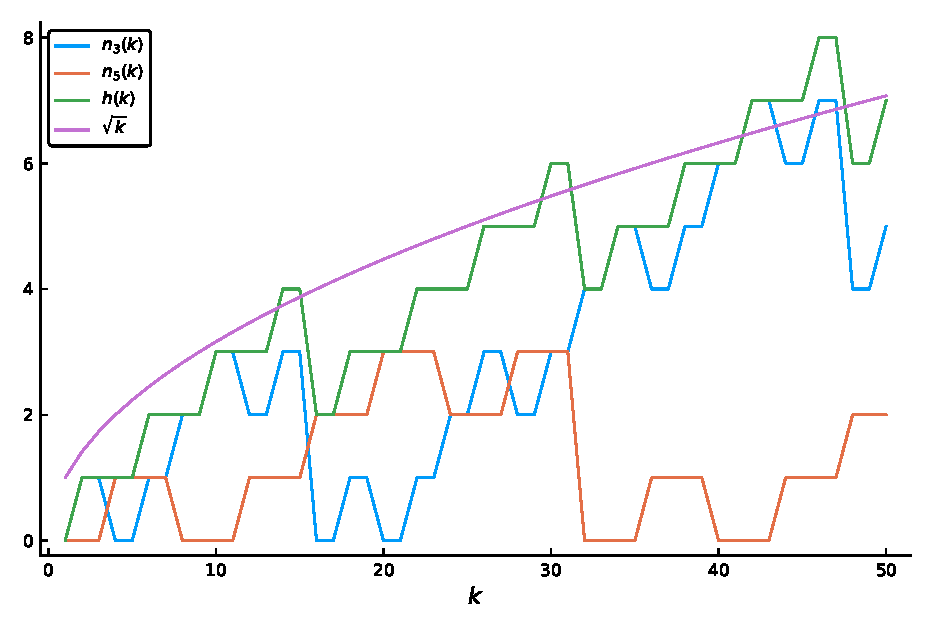
\includegraphics{behaviour_up_to_50}
\end{center}
\paragraph{Range $0$ to $5*10^2$}
\begin{center}
	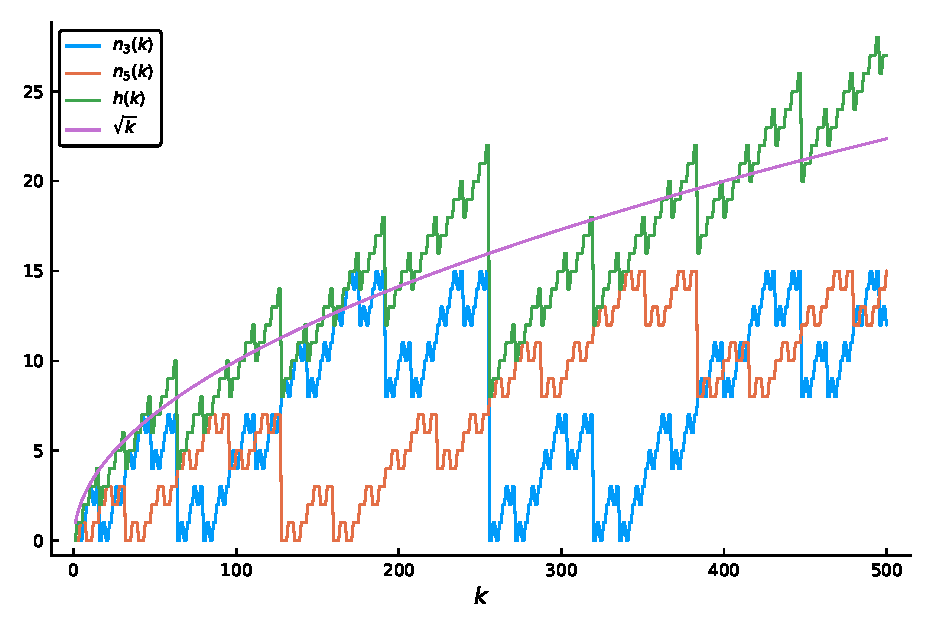
\includegraphics{behaviour_up_to_500}
\end{center}
\newpage
\paragraph{Range $0$ to $5*10^4$}
\begin{center}
	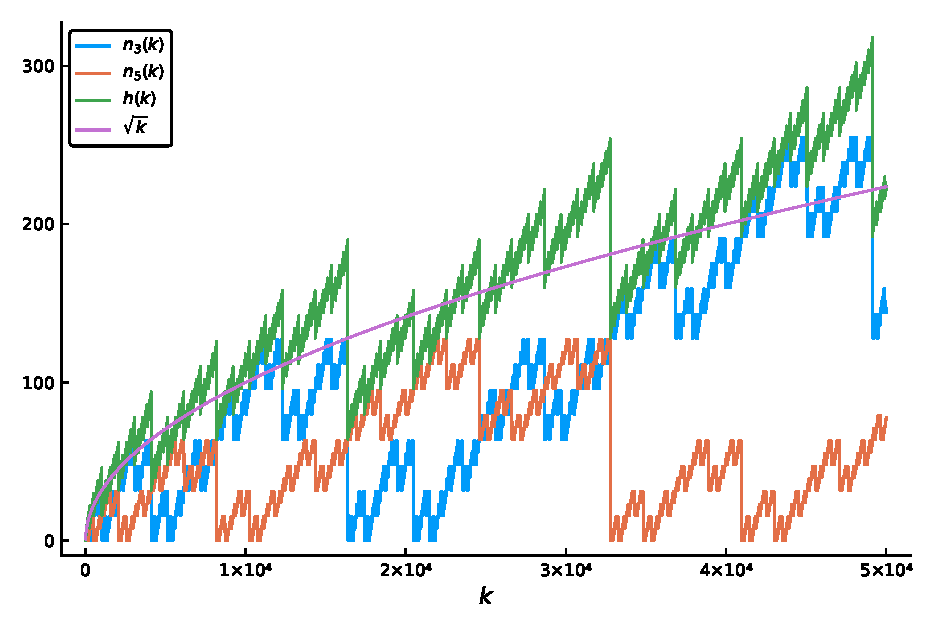
\includegraphics{behaviour_up_to_50000}
\end{center}
\paragraph{Range $0$ to $5*10^7$}
\begin{center}
	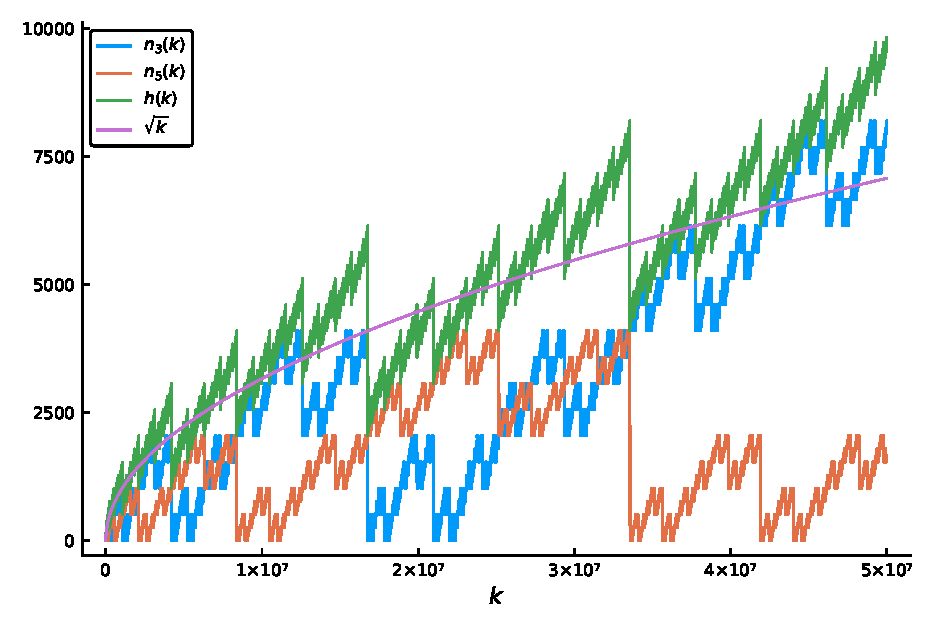
\includegraphics{behaviour_up_to_50000000}
\end{center}
Other pictures (including animated ones) may be found \href{https://pauldubois98.github.io/HeckeOperatorsModuloTwo/behaviour_h/}{online} at \url{https://pauldubois98.github.io/HeckeOperatorsModuloTwo/behaviour_h/}.



\newpage
\paragraph{Integers with Small Code}
\subparagraph{Table}
\label{table:CodeToIntegers}
As the codes of integers are in bijection with even numbers (or odd numbers), we can also plot even (or odd) integers as function of their code.
\begin{center}
	\begin{tabular}{|c||c|c|c|c|c|c|c|c|c|c|c|c|c|c|c|c|}
		\hline
		\textbf{} & \textbf{0} & \textbf{1} & \textbf{2} & \textbf{3} & \textbf{4} & \textbf{5} & \textbf{6} & \textbf{7} & \textbf{8} & \textbf{9} & \textbf{10} & \textbf{11} & \textbf{12} & \textbf{13} & \textbf{14} & \textbf{15} \\
		\hline\hline
		\textbf{0} & 0 & 4 & 16 & 20 & 64 & 68 & 80 & 84 & 256 & 260 & 272 & 276 & 320 & 324 & 336 & 340 \\
		\textbf{1} & 2 & 6 & 18 & 22 & 66 & 70 & 82 & 86 & 258 & 262 & 274 & 278 & 322 & 326 & 338 & 342 \\
		\textbf{2} & 8 & 12 & 24 & 28 & 72 & 76 & 88 & 92 & 264 & 268 & 280 & 284 & 328 & 332 & 344 & 348 \\
		\textbf{3} & 10 & 14 & 26 & 30 & 74 & 78 & 90 & 94 & 266 & 270 & 282 & 286 & 330 & 334 & 346 & 350 \\
		\textbf{4} & 32 & 36 & 48 & 52 & 96 & 100 & 112 & 116 & 288 & 292 & 304 & 308 & 352 & 356 & 368 & 372 \\
		\textbf{5} & 34 & 38 & 50 & 54 & 98 & 102 & 114 & 118 & 290 & 294 & 306 & 310 & 354 & 358 & 370 & 374 \\
		\textbf{6} & 40 & 44 & 56 & 60 & 104 & 108 & 120 & 124 & 296 & 300 & 312 & 316 & 360 & 364 & 376 & 380 \\
		\textbf{7} & 42 & 46 & 58 & 62 & 106 & 110 & 122 & 126 & 298 & 302 & 314 & 318 & 362 & 366 & 378 & 382 \\
		\textbf{8} & 128 & 132 & 144 & 148 & 192 & 196 & 208 & 212 & 384 & 388 & 400 & 404 & 448 & 452 & 464 & 468 \\
		\textbf{9} & 130 & 134 & 146 & 150 & 194 & 198 & 210 & 214 & 386 & 390 & 402 & 406 & 450 & 454 & 466 & 470 \\
		\textbf{10} & 136 & 140 & 152 & 156 & 200 & 204 & 216 & 220 & 392 & 396 & 408 & 412 & 456 & 460 & 472 & 476 \\
		%\textbf{11} & 138 & 142 & 154 & 158 & 202 & 206 & 218 & 222 & 394 & 398 & 410 & 414 & 458 & 462 & 474 & 478 \\
		%\textbf{12} & 160 & 164 & 176 & 180 & 224 & 228 & 240 & 244 & 416 & 420 & 432 & 436 & 480 & 484 & 496 & 500 \\
		%\textbf{13} & 162 & 166 & 178 & 182 & 226 & 230 & 242 & 246 & 418 & 422 & 434 & 438 & 482 & 486 & 498 & 502 \\
		%\textbf{14} & 168 & 172 & 184 & 188 & 232 & 236 & 248 & 252 & 424 & 428 & 440 & 444 & 488 & 492 & 504 & 508 \\
		%\textbf{15} & 170 & 174 & 186 & 190 & 234 & 238 & 250 & 254 & 426 & 430 & 442 & 446 & 490 & 494 & 506 & 510 \\
		\hline
	\end{tabular}
\end{center}
A larger table may be found \href{https://pauldubois98.github.io/HeckeOperatorsModuloTwo/code_to_even/}{online} at \url{https://pauldubois98.github.io/HeckeOperatorsModuloTwo/code_to_even/}.
Note that the same table may be produced for odd integers, find it  \href{https://pauldubois98.github.io/HeckeOperatorsModuloTwo/code_to_odd/}{online} at \url{https://pauldubois98.github.io/HeckeOperatorsModuloTwo/code_to_odd/}.



\subparagraph{Plots}
\label{plot:CodeSurface}
We plot the surface $z = \left[ x, y \right]$ i.e. $z$ is the integer with code $\left[ x, y \right]$.
\begin{center}
	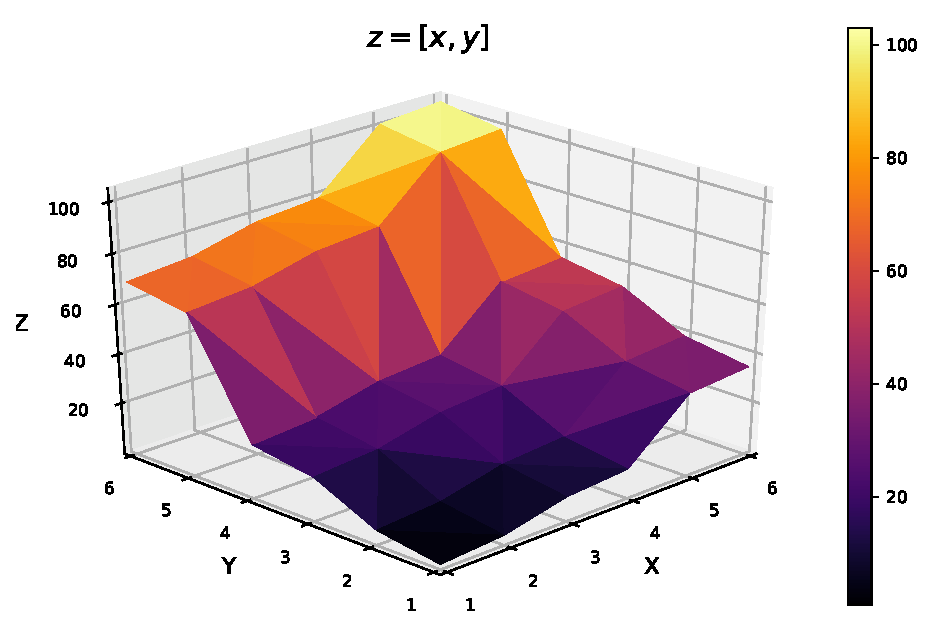
\includegraphics{code_plot_5-5}
\end{center}
\begin{center}
	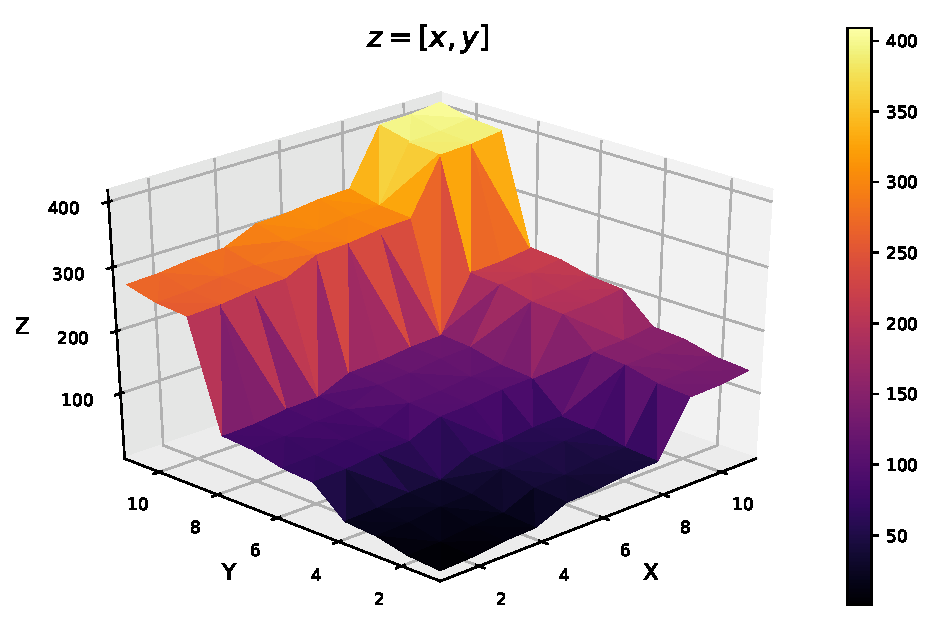
\includegraphics{code_plot_10-10}
\end{center}
\begin{center}
	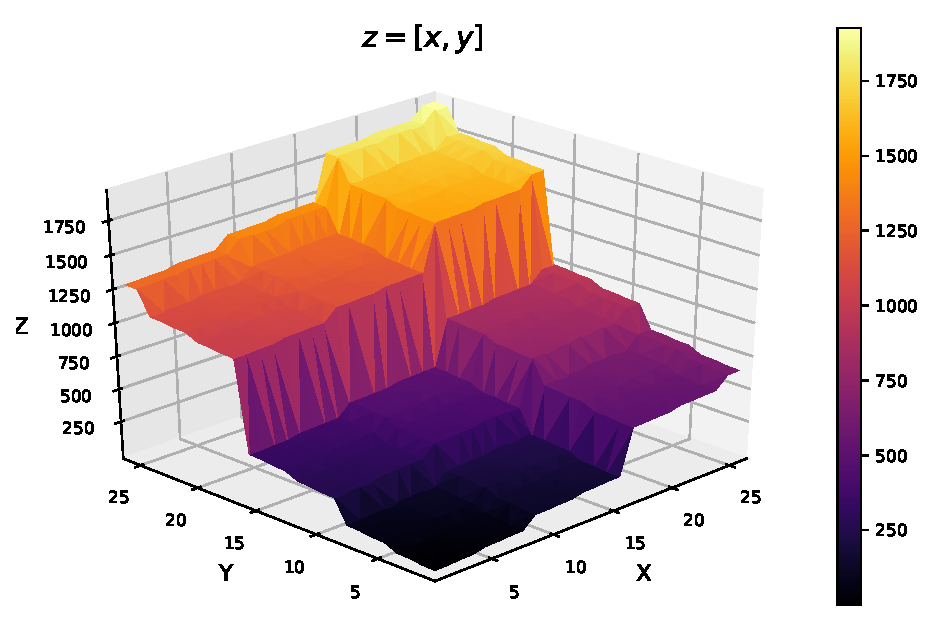
\includegraphics{code_plot_25-25}
\end{center}
Other pictures (including animated ones) may be found \href{https://pauldubois98.github.io/HeckeOperatorsModuloTwo/plot_code_to_int/}{online} at \url{https://pauldubois98.github.io/HeckeOperatorsModuloTwo/plot_code_to_int/}.



\newgeometry{margin=0.5cm, top=2cm, bottom=2cm}
\paragraph{Powers of $T_3$ and $T_5$ giving $\Delta^1$}
\label{table:OperatorToDelta1}
Here, wee look at the power of $\Delta^k$ such that when $T_3^aT_5^b$ is applied to it, we have $T_3^aT_5^b|\Delta^k = \Delta^1$.
\begin{center}
	\begin{tabular}{|c||c|c|c|c|c|c|c|c|c|c|c|c|c|c|c|}
		\hline
		\textbf{} & \textbf{$T_5^{0}$} & \textbf{$T_5^{1}$} & \textbf{$T_5^{2}$} & \textbf{$T_5^{3}$} & \textbf{$T_5^{4}$} & \textbf{$T_5^{5}$} & \textbf{$T_5^{6}$} & \textbf{$T_5^{7}$} & \textbf{$T_5^{8}$} & \textbf{$T_5^{9}$} & \textbf{$T_5^{10}$} & \textbf{$T_5^{11}$} & \textbf{$T_5^{12}$} & \textbf{$T_5^{13}$} & \textbf{$T_5^{14}$} \\
		\hline\hline
		$T_3^{0}$ & $\Delta^{1}$ & $\Delta^{5}$ & $\Delta^{17}$ & $\Delta^{21}$ & $\Delta^{65}$ & $\Delta^{69}$ & $\Delta^{81}$ & $\Delta^{85}$ & $\Delta^{257}$ & $\Delta^{261}$ & $\Delta^{273}$ & $\Delta^{277}$ & $\Delta^{321}$ & $\Delta^{325}$ & $\Delta^{337}$ \\
		$T_3^{1}$ & $\Delta^{3}$ & $\Delta^{7}$ & $\Delta^{19}$ & $\Delta^{23}$ & $\Delta^{67}$ & $\Delta^{71}$ & $\Delta^{83}$ & $\Delta^{87}$ & $\Delta^{259}$ & $\Delta^{263}$ & $\Delta^{275}$ & $\Delta^{279}$ & $\Delta^{323}$ & $\Delta^{327}$ & $\Delta^{339}$ \\
		$T_3^{2}$ & $\Delta^{9}$ & $\Delta^{13}$ & $\Delta^{25}$ & $\Delta^{29}$ & $\Delta^{73}$ & $\Delta^{77}$ & $\Delta^{89}$ & $\Delta^{93}$ & $\Delta^{265}$ & $\Delta^{269}$ & $\Delta^{281}$ & $\Delta^{285}$ & $\Delta^{329}$ & $\Delta^{333}$ & $\Delta^{345}$ \\
		$T_3^{3}$ & $\Delta^{11}$ & $\Delta^{15}$ & $\Delta^{27}$ & $\Delta^{31}$ & $\Delta^{75}$ & $\Delta^{79}$ & $\Delta^{91}$ & $\Delta^{95}$ & $\Delta^{267}$ & $\Delta^{271}$ & $\Delta^{283}$ & $\Delta^{287}$ & $\Delta^{331}$ & $\Delta^{335}$ & $\Delta^{347}$ \\
		$T_3^{4}$ & $\Delta^{33}$ & $\Delta^{37}$ & $\Delta^{49}$ & $\Delta^{53}$ & $\Delta^{97}$ & $\Delta^{101}$ & $\Delta^{113}$ & $\Delta^{117}$ 
		& $\Delta^{289}$ & $\Delta^{293}$ & $\Delta^{305}$ & $\Delta^{309}$ & $\Delta^{353}$ & $\Delta^{357}$ & $\Delta^{369}$ \\
		$T_3^{5}$ & $\Delta^{35}$ & $\Delta^{39}$ & $\Delta^{51}$ & $\Delta^{55}$ & $\Delta^{99}$ & $\Delta^{103}$ & $\Delta^{115}$ & $\Delta^{119}$ 
		& $\Delta^{291}$ & $\Delta^{295}$ & $\Delta^{307}$ & $\Delta^{311}$ & $\Delta^{355}$ & $\Delta^{359}$ & $\Delta^{371}$ \\
		$T_3^{6}$ & $\Delta^{41}$ & $\Delta^{45}$ & $\Delta^{57}$ & $\Delta^{61}$ & $\Delta^{105}$ & $\Delta^{109}$ & $\Delta^{121}$ & $\Delta^{125}$ & $\Delta^{297}$ & $\Delta^{301}$ & $\Delta^{313}$ & $\Delta^{317}$ & $\Delta^{361}$ & $\Delta^{365}$ & $\Delta^{377}$ \\
		$T_3^{7}$ & $\Delta^{43}$ & $\Delta^{47}$ & $\Delta^{59}$ & $\Delta^{63}$ & $\Delta^{107}$ & $\Delta^{111}$ & $\Delta^{123}$ & $\Delta^{127}$ & $\Delta^{299}$ & $\Delta^{303}$ & $\Delta^{315}$ & $\Delta^{319}$ & $\Delta^{363}$ & $\Delta^{367}$ & $\Delta^{379}$ \\
		$T_3^{8}$ & $\Delta^{129}$ & $\Delta^{133}$ & $\Delta^{145}$ & $\Delta^{149}$ & $\Delta^{193}$ & $\Delta^{197}$ & $\Delta^{209}$ & $\Delta^{213}$ & $\Delta^{385}$ & $\Delta^{389}$ & $\Delta^{401}$ & $\Delta^{405}$ & $\Delta^{449}$ & $\Delta^{453}$ & $\Delta^{465}$ \\
		$T_3^{9}$ & $\Delta^{131}$ & $\Delta^{135}$ & $\Delta^{147}$ & $\Delta^{151}$ & $\Delta^{195}$ & $\Delta^{199}$ & $\Delta^{211}$ & $\Delta^{215}$ & $\Delta^{387}$ & $\Delta^{391}$ & $\Delta^{403}$ & $\Delta^{407}$ & $\Delta^{451}$ & $\Delta^{455}$ & $\Delta^{467}$ \\
		$T_3^{10}$ & $\Delta^{137}$ & $\Delta^{141}$ & $\Delta^{153}$ & $\Delta^{157}$ & $\Delta^{201}$ & $\Delta^{205}$ & $\Delta^{217}$ & $\Delta^{221}$ & $\Delta^{393}$ & $\Delta^{397}$ & $\Delta^{409}$ & $\Delta^{413}$ & $\Delta^{457}$ & $\Delta^{461}$ & $\Delta^{473}$ \\
		$T_3^{11}$ & $\Delta^{139}$ & $\Delta^{143}$ & $\Delta^{155}$ & $\Delta^{159}$ & $\Delta^{203}$ & $\Delta^{207}$ & $\Delta^{219}$ & $\Delta^{223}$ & $\Delta^{395}$ & $\Delta^{399}$ & $\Delta^{411}$ & $\Delta^{415}$ & $\Delta^{459}$ & $\Delta^{463}$ & $\Delta^{475}$ \\
		$T_3^{12}$ & $\Delta^{161}$ & $\Delta^{165}$ & $\Delta^{177}$ & $\Delta^{181}$ & $\Delta^{225}$ & $\Delta^{229}$ & $\Delta^{241}$ & $\Delta^{245}$ & $\Delta^{417}$ & $\Delta^{421}$ & $\Delta^{433}$ & $\Delta^{437}$ & $\Delta^{481}$ & $\Delta^{485}$ & $\Delta^{497}$ \\
		$T_3^{13}$ & $\Delta^{163}$ & $\Delta^{167}$ & $\Delta^{179}$ & $\Delta^{183}$ & $\Delta^{227}$ & $\Delta^{231}$ & $\Delta^{243}$ & $\Delta^{247}$ & $\Delta^{419}$ & $\Delta^{423}$ & $\Delta^{435}$ & $\Delta^{439}$ & $\Delta^{483}$ & $\Delta^{487}$ & $\Delta^{499}$ \\
		$T_3^{14}$ & $\Delta^{169}$ & $\Delta^{173}$ & $\Delta^{185}$ & $\Delta^{189}$ & $\Delta^{233}$ & $\Delta^{237}$ & $\Delta^{249}$ & $\Delta^{253}$ & $\Delta^{425}$ & $\Delta^{429}$ & $\Delta^{441}$ & $\Delta^{445}$ & $\Delta^{489}$ & $\Delta^{493}$ & $\Delta^{505}$ \\
		$T_3^{15}$ & $\Delta^{171}$ & $\Delta^{175}$ & $\Delta^{187}$ & $\Delta^{191}$ & $\Delta^{235}$ & $\Delta^{239}$ & $\Delta^{251}$ & $\Delta^{255}$ & $\Delta^{427}$ & $\Delta^{431}$ & $\Delta^{443}$ & $\Delta^{447}$ & $\Delta^{491}$ & $\Delta^{495}$ & $\Delta^{507}$ \\
		$T_3^{16}$ & $\Delta^{513}$ & $\Delta^{517}$ & $\Delta^{529}$ & $\Delta^{533}$ & $\Delta^{577}$ & $\Delta^{581}$ & $\Delta^{593}$ & $\Delta^{597}$ & $\Delta^{769}$ & $\Delta^{773}$ & $\Delta^{785}$ & $\Delta^{789}$ & $\Delta^{833}$ & $\Delta^{837}$ & $\Delta^{849}$ \\
		$T_3^{17}$ & $\Delta^{515}$ & $\Delta^{519}$ & $\Delta^{531}$ & $\Delta^{535}$ & $\Delta^{579}$ & $\Delta^{583}$ & $\Delta^{595}$ & $\Delta^{599}$ & $\Delta^{771}$ & $\Delta^{775}$ & $\Delta^{787}$ & $\Delta^{791}$ & $\Delta^{835}$ & $\Delta^{839}$ & $\Delta^{851}$ \\
		$T_3^{18}$ & $\Delta^{521}$ & $\Delta^{525}$ & $\Delta^{537}$ & $\Delta^{541}$ & $\Delta^{585}$ & $\Delta^{589}$ & $\Delta^{601}$ & $\Delta^{605}$ & $\Delta^{777}$ & $\Delta^{781}$ & $\Delta^{793}$ & $\Delta^{797}$ & $\Delta^{841}$ & $\Delta^{845}$ & $\Delta^{857}$ \\
		$T_3^{19}$ & $\Delta^{523}$ & $\Delta^{527}$ & $\Delta^{539}$ & $\Delta^{543}$ & $\Delta^{587}$ & $\Delta^{591}$ & $\Delta^{603}$ & $\Delta^{607}$ & $\Delta^{779}$ & $\Delta^{783}$ & $\Delta^{795}$ & $\Delta^{799}$ & $\Delta^{843}$ & $\Delta^{847}$ & $\Delta^{859}$ \\
		$T_3^{20}$ & $\Delta^{545}$ & $\Delta^{549}$ & $\Delta^{561}$ & $\Delta^{565}$ & $\Delta^{609}$ & $\Delta^{613}$ & $\Delta^{625}$ & $\Delta^{629}$ & $\Delta^{801}$ & $\Delta^{805}$ & $\Delta^{817}$ & $\Delta^{821}$ & $\Delta^{865}$ & $\Delta^{869}$ & $\Delta^{881}$ \\
		$T_3^{21}$ & $\Delta^{547}$ & $\Delta^{551}$ & $\Delta^{563}$ & $\Delta^{567}$ & $\Delta^{611}$ & $\Delta^{615}$ & $\Delta^{627}$ & $\Delta^{631}$ & $\Delta^{803}$ & $\Delta^{807}$ & $\Delta^{819}$ & $\Delta^{823}$ & $\Delta^{867}$ & $\Delta^{871}$ & $\Delta^{883}$ \\
		$T_3^{22}$ & $\Delta^{553}$ & $\Delta^{557}$ & $\Delta^{569}$ & $\Delta^{573}$ & $\Delta^{617}$ & $\Delta^{621}$ & $\Delta^{633}$ & $\Delta^{637}$ & $\Delta^{809}$ & $\Delta^{813}$ & $\Delta^{825}$ & $\Delta^{829}$ & $\Delta^{873}$ & $\Delta^{877}$ & $\Delta^{889}$ \\
		$T_3^{23}$ & $\Delta^{555}$ & $\Delta^{559}$ & $\Delta^{571}$ & $\Delta^{575}$ & $\Delta^{619}$ & $\Delta^{623}$ & $\Delta^{635}$ & $\Delta^{639}$ & $\Delta^{811}$ & $\Delta^{815}$ & $\Delta^{827}$ & $\Delta^{831}$ & $\Delta^{875}$ & $\Delta^{879}$ & $\Delta^{891}$ \\
		$T_3^{24}$ & $\Delta^{641}$ & $\Delta^{645}$ & $\Delta^{657}$ & $\Delta^{661}$ & $\Delta^{705}$ & $\Delta^{709}$ & $\Delta^{721}$ & $\Delta^{725}$ & $\Delta^{897}$ & $\Delta^{901}$ & $\Delta^{913}$ & $\Delta^{917}$ & $\Delta^{961}$ & $\Delta^{965}$ & $\Delta^{977}$ \\
		$T_3^{25}$ & $\Delta^{643}$ & $\Delta^{647}$ & $\Delta^{659}$ & $\Delta^{663}$ & $\Delta^{707}$ & $\Delta^{711}$ & $\Delta^{723}$ & $\Delta^{727}$ & $\Delta^{899}$ & $\Delta^{903}$ & $\Delta^{915}$ & $\Delta^{919}$ & $\Delta^{963}$ & $\Delta^{967}$ & $\Delta^{979}$ \\
		$T_3^{26}$ & $\Delta^{649}$ & $\Delta^{653}$ & $\Delta^{665}$ & $\Delta^{669}$ & $\Delta^{713}$ & $\Delta^{717}$ & $\Delta^{729}$ & $\Delta^{733}$ & $\Delta^{905}$ & $\Delta^{909}$ & $\Delta^{921}$ & $\Delta^{925}$ & $\Delta^{969}$ & $\Delta^{973}$ & $\Delta^{985}$ \\
		$T_3^{27}$ & $\Delta^{651}$ & $\Delta^{655}$ & $\Delta^{667}$ & $\Delta^{671}$ & $\Delta^{715}$ & $\Delta^{719}$ & $\Delta^{731}$ & $\Delta^{735}$ & $\Delta^{907}$ & $\Delta^{911}$ & $\Delta^{923}$ & $\Delta^{927}$ & $\Delta^{971}$ & $\Delta^{975}$ & $\Delta^{987}$ \\
		$T_3^{28}$ & $\Delta^{673}$ & $\Delta^{677}$ & $\Delta^{689}$ & $\Delta^{693}$ & $\Delta^{737}$ & $\Delta^{741}$ & $\Delta^{753}$ & $\Delta^{757}$ & $\Delta^{929}$ & $\Delta^{933}$ & $\Delta^{945}$ & $\Delta^{949}$ & $\Delta^{993}$ & $\Delta^{997}$ & $\Delta^{1009}$ \\
		$T_3^{29}$ & $\Delta^{675}$ & $\Delta^{679}$ & $\Delta^{691}$ & $\Delta^{695}$ & $\Delta^{739}$ & $\Delta^{743}$ & $\Delta^{755}$ & $\Delta^{759}$ & $\Delta^{931}$ & $\Delta^{935}$ & $\Delta^{947}$ & $\Delta^{951}$ & $\Delta^{995}$ & $\Delta^{999}$ & $\Delta^{1011}$ \\
		$T_3^{30}$ & $\Delta^{681}$ & $\Delta^{685}$ & $\Delta^{697}$ & $\Delta^{701}$ & $\Delta^{745}$ & $\Delta^{749}$ & $\Delta^{761}$ & $\Delta^{765}$ & $\Delta^{937}$ & $\Delta^{941}$ & $\Delta^{953}$ & $\Delta^{957}$ & $\Delta^{1001}$ & $\Delta^{1005}$ & $\Delta^{1017}$ \\
		\hline
	\end{tabular}
\end{center}
A larger table may be found \href{https://pauldubois98.github.io/HeckeOperatorsModuloTwo/T3T5_powers_to_delta/}{online} at \url{https://pauldubois98.github.io/HeckeOperatorsModuloTwo/T3T5_powers_to_delta/}.



\newgeometry{margin=2cm}
\subsection{Expansions of $T_p$ as Series of $T_3$ and $T_5$}
\label{expansionsOfTp}
Here are expansions of $T_p$ in series of $T_3^aT_5^b$ for primes $p<80$:\\
$T_{3} = T_3^{1}T_5^{0}$\\
$T_{5} = T_3^{0}T_5^{1}$\\
$T_{7} = T_3^{1}T_5^{1} + T_3^{3}T_5^{1} + T_3^{3}T_5^{3} + T_3^{5}T_5^{1} + T_3^{1}T_5^{7} + T_3^{1}T_5^{9} + T_3^{7}T_5^{3} + T_3^{7}T_5^{5} + T_3^{9}T_5^{3} + T_3^{11}T_5^{1} + T_3^{3}T_5^{11} + T_3^{5}T_5^{9} + T_3^{13}T_5^{1} + T_3^{3}T_5^{13} + T_3^{5}T_5^{11} + T_3^{9}T_5^{7} + T_3^{11}T_5^{5} + T_3^{13}T_5^{3} + T_3^{3}T_5^{15} + T_3^{7}T_5^{11} + T_3^{9}T_5^{9} + T_3^{13}T_5^{5} + T_3^{15}T_5^{3} + \dots $\\   
$T_{11} = T_3^{1}T_5^{0} + T_3^{1}T_5^{2} + T_3^{3}T_5^{0} + T_3^{1}T_5^{4} + T_3^{3}T_5^{2} + T_3^{5}T_5^{0} + T_3^{1}T_5^{6} + T_3^{3}T_5^{4} + T_3^{7}T_5^{2} + T_3^{1}T_5^{10} + T_3^{3}T_5^{8} + T_3^{7}T_5^{4} + T_3^{9}T_5^{2} + T_3^{11}T_5^{2} + T_3^{3}T_5^{12} + T_3^{5}T_5^{10} + T_3^{7}T_5^{8} + T_3^{11}T_5^{4} + T_3^{13}T_5^{2} + T_3^{9}T_5^{8} + T_3^{17}T_5^{0} + \dots $\\
$T_{13} = T_3^{0}T_5^{1} + T_3^{0}T_5^{3} + T_3^{2}T_5^{1} + T_3^{0}T_5^{5} + T_3^{4}T_5^{1} + T_3^{2}T_5^{5} + T_3^{4}T_5^{3} + T_3^{6}T_5^{1} + T_3^{0}T_5^{9} + T_3^{2}T_5^{7} + T_3^{6}T_5^{3} + T_3^{0}T_5^{11} + T_3^{6}T_5^{5} + T_3^{8}T_5^{3} + T_3^{10}T_5^{1} + T_3^{2}T_5^{11} + T_3^{4}T_5^{9} + T_3^{6}T_5^{7} + T_3^{10}T_5^{3} + T_3^{2}T_5^{13} + T_3^{4}T_5^{11} + T_3^{14}T_5^{1} + T_3^{2}T_5^{15} + T_3^{4}T_5^{13} + T_3^{6}T_5^{11} + T_3^{12}T_5^{5} + T_3^{16}T_5^{1} + \dots $\\
$T_{17} = T_3^{0}T_5^{2} + T_3^{2}T_5^{0} + T_3^{2}T_5^{2} + T_3^{0}T_5^{6} + T_3^{4}T_5^{2} + T_3^{6}T_5^{0} + T_3^{2}T_5^{6} + T_3^{4}T_5^{4} + T_3^{6}T_5^{2} + T_3^{10}T_5^{0} + T_3^{2}T_5^{10} + T_3^{4}T_5^{8} + T_3^{6}T_5^{6} + T_3^{10}T_5^{2} + T_3^{2}T_5^{12} + T_3^{6}T_5^{8} + T_3^{10}T_5^{4} + T_3^{2}T_5^{14} + T_3^{6}T_5^{10} + T_3^{8}T_5^{8} + T_3^{12}T_5^{4} + T_3^{14}T_5^{2} + T_3^{4}T_5^{14} + T_3^{8}T_5^{10} + T_3^{10}T_5^{8} + T_3^{12}T_5^{6} + T_3^{16}T_5^{2} + T_3^{18}T_5^{0} + \dots $\\
$T_{19} = T_3^{1}T_5^{0} + T_3^{3}T_5^{0} + T_3^{1}T_5^{4} + T_3^{3}T_5^{2} + T_3^{1}T_5^{6} + T_3^{5}T_5^{2} + T_3^{3}T_5^{6} + T_3^{7}T_5^{2} + T_3^{9}T_5^{0} + T_3^{1}T_5^{10} + T_3^{7}T_5^{4} + T_3^{9}T_5^{2} + T_3^{11}T_5^{0} + T_3^{1}T_5^{12} + T_3^{5}T_5^{8} + T_3^{11}T_5^{2} + T_3^{13}T_5^{0} + T_3^{3}T_5^{12} + T_3^{7}T_5^{8} + T_3^{9}T_5^{6} + T_3^{11}T_5^{4} + T_3^{13}T_5^{2} + T_3^{3}T_5^{14} + T_3^{7}T_5^{10} + T_3^{11}T_5^{6} + T_3^{15}T_5^{2} + T_3^{17}T_5^{0} + \dots $\\
$T_{23} = T_3^{1}T_5^{1} + T_3^{1}T_5^{3} + T_3^{5}T_5^{1} + T_3^{1}T_5^{7} + T_3^{5}T_5^{5} + T_3^{7}T_5^{3} + T_3^{1}T_5^{13} + T_3^{5}T_5^{9} + T_3^{7}T_5^{7} + T_3^{1}T_5^{15} + T_3^{3}T_5^{13} + T_3^{5}T_5^{11} + T_3^{7}T_5^{9} + T_3^{11}T_5^{5} + T_3^{13}T_5^{3} + T_3^{15}T_5^{1} + T_3^{17}T_5^{1} + \dots $\\
$T_{29} = T_3^{0}T_5^{1} + T_3^{0}T_5^{3} + T_3^{2}T_5^{3} + T_3^{2}T_5^{5} + T_3^{6}T_5^{1} + T_3^{0}T_5^{9} + T_3^{0}T_5^{11} + T_3^{2}T_5^{9} + T_3^{4}T_5^{7} + T_3^{8}T_5^{3} + T_3^{0}T_5^{13} + T_3^{6}T_5^{7} + T_3^{10}T_5^{3} + T_3^{12}T_5^{1} + T_3^{2}T_5^{13} + T_3^{8}T_5^{7} + T_3^{4}T_5^{13} + T_3^{6}T_5^{11} + T_3^{12}T_5^{5} + T_3^{14}T_5^{3} + T_3^{16}T_5^{1} + \dots $\\
$T_{31} = T_3^{1}T_5^{1} + T_3^{1}T_5^{3} + T_3^{3}T_5^{3} + T_3^{5}T_5^{1} + T_3^{3}T_5^{5} + T_3^{1}T_5^{9} + T_3^{1}T_5^{11} + T_3^{9}T_5^{3} + T_3^{11}T_5^{1} + T_3^{1}T_5^{13} + T_3^{3}T_5^{11} + T_3^{9}T_5^{5} + T_3^{1}T_5^{15} + T_3^{9}T_5^{7} + T_3^{15}T_5^{1} + T_3^{13}T_5^{5} + T_3^{15}T_5^{3} + \dots $\\
$T_{37} = T_3^{0}T_5^{1} + T_3^{0}T_5^{3} + T_3^{2}T_5^{1} + T_3^{2}T_5^{3} + T_3^{2}T_5^{5} + T_3^{4}T_5^{3} + T_3^{2}T_5^{7} + T_3^{6}T_5^{3} + T_3^{8}T_5^{1} + T_3^{6}T_5^{5} + T_3^{2}T_5^{11} + T_3^{6}T_5^{7} + T_3^{8}T_5^{5} + T_3^{12}T_5^{1} + T_3^{6}T_5^{9} + T_3^{8}T_5^{7} 
+ T_3^{2}T_5^{15} + T_3^{4}T_5^{13} + T_3^{12}T_5^{5} + \dots $\\
$T_{41} = T_3^{0}T_5^{2} + T_3^{2}T_5^{2} + T_3^{4}T_5^{0} + T_3^{2}T_5^{4} + T_3^{4}T_5^{2} + T_3^{6}T_5^{2} + T_3^{0}T_5^{10} + T_3^{2}T_5^{10} + T_3^{8}T_5^{4} + T_3^{10}T_5^{2} + T_3^{12}T_5^{0} + T_3^{0}T_5^{14} + T_3^{2}T_5^{12} + T_3^{8}T_5^{6} + T_3^{14}T_5^{2} + T_3^{4}T_5^{14} + T_3^{8}T_5^{10} + T_3^{10}T_5^{8} + T_3^{16}T_5^{2} + \dots $\\
$T_{43} = T_3^{1}T_5^{0} + T_3^{3}T_5^{2} + T_3^{5}T_5^{0} + T_3^{1}T_5^{6} + T_3^{3}T_5^{4} + T_3^{5}T_5^{2} + T_3^{7}T_5^{0} + T_3^{7}T_5^{2} + T_3^{5}T_5^{6} + T_3^{9}T_5^{2} + T_3^{5}T_5^{8} + T_3^{9}T_5^{4} + T_3^{3}T_5^{12} + T_3^{5}T_5^{10} + T_3^{9}T_5^{6} + T_3^{11}T_5^{4} + T_3^{3}T_5^{14} + T_3^{5}T_5^{12} + T_3^{9}T_5^{8} + T_3^{11}T_5^{6} + T_3^{13}T_5^{4} + \dots $\\
$T_{47} = T_3^{1}T_5^{1} + T_3^{1}T_5^{5} + T_3^{3}T_5^{3} + T_3^{5}T_5^{1} + T_3^{5}T_5^{3} + T_3^{3}T_5^{7} + T_3^{5}T_5^{5} + T_3^{9}T_5^{1} + T_3^{1}T_5^{11} + T_3^{5}T_5^{7} + T_3^{7}T_5^{5} + T_3^{1}T_5^{13} + T_3^{5}T_5^{9} + T_3^{9}T_5^{5} + T_3^{3}T_5^{13} + T_3^{9}T_5^{7} + T_3^{11}T_5^{5} + T_3^{13}T_5^{3} + T_3^{15}T_5^{1} + T_3^{3}T_5^{15} + T_3^{7}T_5^{11} + T_3^{9}T_5^{9} + T_3^{15}T_5^{3} + \dots $\\    
$T_{53} = T_3^{0}T_5^{1} + T_3^{2}T_5^{1} + T_3^{0}T_5^{5} + T_3^{2}T_5^{3} + T_3^{4}T_5^{1} + T_3^{0}T_5^{7} + T_3^{4}T_5^{3} + T_3^{6}T_5^{1} + T_3^{0}T_5^{9} + T_3^{4}T_5^{5} + T_3^{8}T_5^{1} + T_3^{10}T_5^{1} + T_3^{8}T_5^{5} + T_3^{2}T_5^{13} + T_3^{4}T_5^{11} + T_3^{6}T_5^{9} + T_3^{10}T_5^{5} + T_3^{14}T_5^{1} + T_3^{2}T_5^{15} + T_3^{4}T_5^{13} + T_3^{6}T_5^{11} + T_3^{14}T_5^{3} + T_3^{16}T_5^{1} + \dots $\\   
$T_{59} = T_3^{1}T_5^{0} + T_3^{1}T_5^{2} + T_3^{5}T_5^{0} + T_3^{1}T_5^{6} + T_3^{5}T_5^{2} + T_3^{7}T_5^{0} + T_3^{1}T_5^{8} + T_3^{9}T_5^{0} + T_3^{5}T_5^{6} + T_3^{7}T_5^{4} + T_3^{9}T_5^{2} + T_3^{3}T_5^{10} + T_3^{7}T_5^{6} + T_3^{5}T_5^{10} + T_3^{7}T_5^{8} + T_3^{9}T_5^{6} 
+ T_3^{9}T_5^{8} + T_3^{11}T_5^{6} + \dots $\\
$T_{61} = T_3^{0}T_5^{1} + T_3^{2}T_5^{1} + T_3^{0}T_5^{5} + T_3^{2}T_5^{3} + T_3^{0}T_5^{7} + T_3^{6}T_5^{3} + T_3^{8}T_5^{1} + T_3^{2}T_5^{9} + T_3^{4}T_5^{7} + T_3^{8}T_5^{3} + T_3^{2}T_5^{11} + T_3^{4}T_5^{9} + T_3^{10}T_5^{3} + T_3^{12}T_5^{1} + T_3^{4}T_5^{11} + T_3^{6}T_5^{9} + T_3^{12}T_5^{3} + T_3^{4}T_5^{13} + T_3^{6}T_5^{11} + T_3^{8}T_5^{9} + \dots $\\
$T_{67} = T_3^{1}T_5^{0} + T_3^{1}T_5^{2} + T_3^{3}T_5^{0} + T_3^{1}T_5^{4} + T_3^{5}T_5^{0} + T_3^{3}T_5^{4} + T_3^{3}T_5^{6} + T_3^{7}T_5^{2} + T_3^{9}T_5^{0} + T_3^{1}T_5^{10} + T_3^{3}T_5^{8} + T_3^{5}T_5^{6} + T_3^{9}T_5^{2} + T_3^{11}T_5^{0} + T_3^{3}T_5^{10} + T_3^{5}T_5^{8} + T_3^{7}T_5^{6} + T_3^{9}T_5^{4} + T_3^{1}T_5^{14} + T_3^{3}T_5^{12} + T_3^{5}T_5^{10} + T_3^{7}T_5^{8} + T_3^{9}T_5^{6} + T_3^{5}T_5^{12} 
+ T_3^{9}T_5^{8} + T_3^{11}T_5^{6} + T_3^{13}T_5^{4} + T_3^{15}T_5^{2} + \dots $\\
$T_{71} = T_3^{1}T_5^{1} + T_3^{1}T_5^{3} + T_3^{3}T_5^{5} + T_3^{7}T_5^{1} + T_3^{3}T_5^{7} + T_3^{5}T_5^{5} + T_3^{7}T_5^{5} + T_3^{9}T_5^{3} + T_3^{3}T_5^{11} + T_3^{7}T_5^{7} + T_3^{9}T_5^{5} + T_3^{11}T_5^{3} + T_3^{13}T_5^{1} + T_3^{3}T_5^{13} + T_3^{5}T_5^{11} + T_3^{9}T_5^{7} + T_3^{11}T_5^{5} + T_3^{13}T_5^{3} + T_3^{15}T_5^{1} + T_3^{7}T_5^{11} + T_3^{13}T_5^{5} + \dots $\\
$T_{73} = T_3^{2}T_5^{0} + T_3^{0}T_5^{4} + T_3^{2}T_5^{2} + T_3^{2}T_5^{4} + T_3^{6}T_5^{0} + T_3^{2}T_5^{6} + T_3^{2}T_5^{8} + T_3^{4}T_5^{6} + T_3^{8}T_5^{2} + T_3^{10}T_5^{2} + T_3^{4}T_5^{10} + T_3^{6}T_5^{8} + T_3^{8}T_5^{6} + T_3^{10}T_5^{4} + T_3^{2}T_5^{14} + T_3^{8}T_5^{8} + T_3^{10}T_5^{6} + T_3^{10}T_5^{8} + T_3^{16}T_5^{2} + \dots $\\
$T_{79} = T_3^{1}T_5^{1} + T_3^{1}T_5^{3} + T_3^{3}T_5^{1} + T_3^{1}T_5^{5} + T_3^{1}T_5^{7} + T_3^{7}T_5^{1} + T_3^{1}T_5^{9} + T_3^{7}T_5^{3} + T_3^{1}T_5^{11} + T_3^{9}T_5^{3} + T_3^{1}T_5^{13} + T_3^{3}T_5^{11} + T_3^{5}T_5^{9} + T_3^{7}T_5^{7} + T_3^{9}T_5^{5} + T_3^{11}T_5^{3} + T_3^{3}T_5^{13} + T_3^{7}T_5^{9} + T_3^{11}T_5^{5} + T_3^{15}T_5^{1} + T_3^{3}T_5^{15} + T_3^{5}T_5^{13} + T_3^{9}T_5^{9} + T_3^{11}T_5^{7} + \dots $\\
Expansions for larger primes may be found \href{https://pauldubois98.github.io/HeckeOperatorsModuloTwo/T_p_extensions/}{online} at \url{https://pauldubois98.github.io/HeckeOperatorsModuloTwo/T_p_extensions/}.



	% !TeX spellcheck = en_GB
%\inputminted[firstline=2,lastline=15]{language}{file}

\section{Speed Comparison}
\subsection{Pure Python}
\label{code:PurePython}
\inputminted[lastline=19, breaklines]{python}{SpeedComparison/PurePython.py}

\subsection{NumPy Python}
\label{code:NumPyPython}
\inputminted[lastline=21, breaklines]{python}{SpeedComparison/NumPyPython.py}

\subsection{Dense Julia}
\label{code:DenseJulia}
\inputminted[lastline=24, breaklines]{julia}{SpeedComparison/DenseJulia.jl}

\subsection{Sparse Python}
\label{code:SparsePython}
\inputminted[lastline=18, breaklines]{python}{SpeedComparison/SparsePython.py}

\subsection{Sparse Julia}
\label{code:SparseJulia}
\inputminted[lastline=24, breaklines]{julia}{SpeedComparison/SparseJulia.jl}





\section{ModularFormsModuloTwo.jl}
\subsection[Files Tree]{Module structure}
\dirtree{% Module file tree
	.1 \textit{ModularFormsModuloTwo.jl (module)}.
	.2 docs.
	.3 \textit{(automatic documentation)}.
	.2 examples.
	.3 Hecke\_primes\_table.jl.
	.3 Hecke\_powers\_table.j.
	.2 src.
	.3 data.
	.4 storage.jl.
	.4 delta\_file\_maker.jl.
	.4 Hecke\_primes\_file\_maker.jl.
	.4 Hecke\_powers\_file\_maker.jl.
	.4 \textit{data files (.JLD2)}.
	.3 arithmetic.jl.
	.3 equality.jl.
	.3 generators.jl.
	.3 HeckeOperator.jl.
	.3 ModularFormsModuloTwo.jl.
	.3 recognizer.jl.
}
Full module on \href{https://github.com/pauldubois98/ModularFormsModuloTwo.jl}{GitHub} (\url{https://github.com/pauldubois98/ModularFormsModuloTwo.jl}).
The official \href{https://pauldubois98.github.io/ModularFormsModuloTwo.jl/}{documentation} (\url{https://pauldubois98.github.io/ModularFormsModuloTwo.jl/}) has more details on how to use.

\subsection{Files details}

\subsubsection{\href{https://github.com/pauldubois98/ModularFormsModuloTwo.jl/tree/master/src}{Main Sources}}
\subparagraph{\href{https://github.com/pauldubois98/ModularFormsModuloTwo.jl/blob/master/src/ModularFormsModuloTwo.jl}{ModularFormsModuloTwo.jl}}
\label{code:ModularFormsModuloTwo}
\inputminted[breaklines]{julia}{Module/ModularFormsModuloTwo.jl}

\subparagraph{\href{https://github.com/pauldubois98/ModularFormsModuloTwo.jl/blob/master/src/arithmetic.jl}{arithmetic.jl}}
\label{code:arithmetic}
\inputminted[breaklines]{julia}{Module/arithmetic.jl}

\subparagraph{\href{https://github.com/pauldubois98/ModularFormsModuloTwo.jl/blob/master/src/equality.jl}{equality.jl}}
\label{code:equality}
\inputminted[breaklines]{julia}{Module/equality.jl}

\subparagraph{\href{https://github.com/pauldubois98/ModularFormsModuloTwo.jl/blob/master/src/generators.jl}{generators.jl}}
\label{code:generators}
\inputminted[breaklines]{julia}{Module/generators.jl}

\subparagraph{\href{https://github.com/pauldubois98/ModularFormsModuloTwo.jl/blob/master/src/HeckeOperator.jl}{HeckeOperator.jl}}
\label{code:HeckeOperator}
\inputminted[breaklines]{julia}{Module/HeckeOperator.jl}

\subparagraph{\href{https://github.com/pauldubois98/ModularFormsModuloTwo.jl/blob/master/src/recognizer.jl}{recognizer.jl}}
\label{code:recognizer}
\inputminted[breaklines]{julia}{Module/recognizer.jl}


\subsubsection{\href{https://github.com/pauldubois98/ModularFormsModuloTwo.jl/tree/master/src/data}{Data Submodule}}
\subparagraph{\href{https://github.com/pauldubois98/ModularFormsModuloTwo.jl/blob/master/src/data/storage.jl}{storage.jl}}
\label{code:storage}
\inputminted[breaklines]{julia}{Module/storage.jl}

\subparagraph{\href{https://github.com/pauldubois98/ModularFormsModuloTwo.jl/blob/master/src/data/delta_file_maker.jl}{delta\_file\_maker.jl}}
\label{code:deltaFileMaker}
\inputminted[breaklines]{julia}{Module/deltaFileMaker.jl}

\subparagraph{\href{https://github.com/pauldubois98/ModularFormsModuloTwo.jl/blob/master/src/data/Hecke_primes_file_maker.jl}{Hecke\_primes\_file\_maker.jl}}
\label{code:HeckePrimesFileMaker}
\inputminted[breaklines]{julia}{Module/HeckePrimesFileMaker.jl}

\subparagraph{\href{https://github.com/pauldubois98/ModularFormsModuloTwo.jl/blob/master/src/data/Hecke_powers_file_maker.jl}{Hecke\_powers\_file\_maker.jl}}
\label{code:HeckePowersFileMaker}
\inputminted[breaklines]{julia}{Module/HeckePowersFileMaker.jl}



\section{Other Programs}
	% !TeX spellcheck = en_GB

\section{Governing Fields Results}
\label{governingFieldsResults}
The same results are available \href{https://pauldubois98.github.io/HeckeOperatorsModuloTwo/GoverningFields/}{online} at \url{https://pauldubois98.github.io/HeckeOperatorsModuloTwo/GoverningFields/}.
There are full names for extensions online, for size reason, we will use some variables $\alpha$ and $\beta$ in here.

We will write $\stackrel{?}{=}$ for the fields with strong evidence of being governing fields, and $=$ for the ones we are sure.

\subsection{$a_{0k}$}
Here we look at the maps $a_{0k}$.

\subsubsection{$a_{01}$}
Governing field:
$$M_{01} = \mathbb{Q}\left(\zeta_8\right)$$
\begin{multicols}{2}
	\begin{itemize}
		\item $G_{01} = C_2 \times C_2$
		\item $\abs{S_{01}^1} = 1$
		\item $\abs{C_{01}^1} = 1$
	\end{itemize}
	\begin{itemize}
		\item $\abs{\{ p \in \primes \mid a_{01}(p)=0, p<10^4 \}} = 914$\\
		Ratio: $\nicefrac{ 914 }{ 1228 } \approx \nicefrac{ 3 }{ 4 }$
		\item $\abs{\{ p \in \primes \mid a_{01}(p)=1, p<10^4 \}} = 314$\\
		Ratio: $\nicefrac{ 314 }{ 1228 } \approx \nicefrac{ 1 }{ 4 }$
	\end{itemize}
\end{multicols}

\subsubsection{$a_{02}$}
Governing field:
$$M_{02} = \mathbb{Q}\left(\zeta_8, \sqrt[4]{2}\right)$$
\begin{multicols}{2}
	\begin{itemize}
		\item $G_{02} = D_8$
		\item $\abs{S_{02}^1} = 1$
		\item $\abs{C_{02}^1} = 1$
	\end{itemize}
	\begin{itemize}
		\item $\abs{\{ p \in \primes \mid a_{02}(p)=0, p<10^4 \}} = 1076$\\
		Ratio: $\nicefrac{ 1076 }{ 1228 } \approx \nicefrac{ 7 }{ 8 }$
		\item $\abs{\{ p \in \primes \mid a_{02}(p)=1, p<10^4 \}} = 152$\\
		Ratio: $\nicefrac{ 152 }{ 1228 } \approx \nicefrac{ 1 }{ 8 }$
	\end{itemize}
\end{multicols}

\subsubsection{$a_{03}$}
Governing field:
$$M_{03} \stackrel{?}{=} \mathbb{Q}\left(\zeta_8, \sqrt[4]{2}, \sqrt{\alpha}\right)$$
where:
$$\alpha = - \frac{3136435454775881 \sqrt[4]{2}}{562949953421312} + \frac{4208721080340285 \sqrt{2}}{2251799813685248} + \frac{3672578267558083 \cdot \sqrt[4]{2}^3}{562949953421312} + \frac{3582104167901087}{281474976710656}$$
\begin{multicols}{2}
	\begin{itemize}
		\item $G_{03} = D_{16}$
		\item $\abs{S_{03}^1} = 2$
		\item $\abs{C_{03}^1} = 1$
	\end{itemize}
	\begin{itemize}
		\item $\abs{\{ p \in \primes \mid a_{03}(p)=0, p<10^4 \}} = 1071$\\
		Ratio: $\nicefrac{ 1071 }{ 1228 } \approx \nicefrac{ 14 }{ 16 }$
		\item $\abs{\{ p \in \primes \mid a_{03}(p)=1, p<10^4 \}} = 157$\\
		Ratio: $\nicefrac{ 157 }{ 1228 } \approx \nicefrac{ 2 }{ 16 }$
	\end{itemize}
\end{multicols}

\subsubsection{$a_{04}$}
Same governing field as $a_{03}$, thus also same Galois group ($M_{04} \stackrel{?}{=} M_{03}$ and $G_{04} \stackrel{?}{=} G_{03}$).
\begin{multicols}{2}
	\begin{itemize}
		\item $G_{04} = D_{16}$
		\item $\abs{S_{04}^1} = 1$
		\item $\abs{C_{04}^1} = 1$
	\end{itemize}
	\begin{itemize}
		\item $\abs{\{ p \in \primes \mid a_{04}(p)=0, p<10^4 \}} = 1155$\\
		Ratio: $\nicefrac{ 1155 }{ 1228 } \approx \nicefrac{ 15 }{ 16 }$
		\item $\abs{\{ p \in \primes \mid a_{04}(p)=1, p<10^4 \}} = 73$\\
		Ratio: $\nicefrac{ 73 }{ 1228 } \approx \nicefrac{ 1 }{ 16 }$
	\end{itemize}
\end{multicols}

\subsubsection{$a_{05}$}
Governing field:
$$\mathbb{Q}\left(\zeta_8, \sqrt[4]{2}, \sqrt{\alpha}, \sqrt{\beta}\right)$$
where:
$$\alpha = - \frac{3136435454775881 \sqrt[4]{2}}{562949953421312} + \frac{4208721080340285 \sqrt{2}}{2251799813685248} + \frac{3672578267558083 \cdot \sqrt[4]{2}^3}{562949953421312} + \frac{3582104167901087}{281474976710656}$$
and
\begin{align*}
\beta = 
&- \frac{8282936156772053 \alpha^{\frac{13}{2}}}{1125899906842624} 
- \frac{1240182980093567 \alpha^{6}}{562949953421312} 
- \frac{336382584949535 \alpha^{\frac{9}{2}}}{2199023255552} 
\\
&- \frac{6445823996745319 \alpha^{4}}{140737488355328} 
- \frac{4638634719581101 \alpha^{\frac{5}{2}}}{35184372088832} 
- \frac{2954723016803317 \alpha^{2}}{70368744177664} 
\\
&- \frac{5142889464378747 \sqrt[4]{2}}{140737488355328} 
- \frac{4198844765367981 \sqrt{\alpha}}{1125899906842624} 
+ \frac{3450571136356681 \sqrt{2}}{281474976710656} 
\\
&+ \frac{6022015868546055 \cdot \sqrt[4]{2}^3}{140737488355328} 
+ \frac{5763554133419461}{70368744177664} 
+ \frac{7633450872164841 \alpha^{\frac{3}{2}}}{281474976710656} 
\\
&+ \frac{615248862392953 \alpha^{3}}{8796093022208} 
+ \frac{8240373942248553 \alpha^{\frac{7}{2}}}{35184372088832} 
+ \frac{8030384673908857 \alpha^{5}}{562949953421312} 
\\
&+ \frac{4981425151744809 \alpha^{7}}{18014398509481984} 
+ \frac{1676680829315919 \alpha^{\frac{11}{2}}}{35184372088832} 
+ \frac{8299866982438859 \alpha^{\frac{15}{2}}}{9007199254740992}
\end{align*}
\begin{multicols}{2}
	\begin{itemize}
		\item $G_{265} = D_{32}$
		\item $\abs{S_{265}^1} = 4$
		\item $\abs{C_{265}^1} = 2$
	\end{itemize}
	\begin{itemize}
		\item $\abs{\{ p \in \primes \mid a_{265}(p)=0, p<10^4 \}} = 1069$\\
		Ratio: $\nicefrac{ 1069 }{ 1228 } \approx \nicefrac{ 28 }{ 32 }$
		\item $\abs{\{ p \in \primes \mid a_{265}(p)=1, p<10^4 \}} = 159$\\
		Ratio: $\nicefrac{ 159 }{ 1228 } \approx \nicefrac{ 4 }{ 32 }$
	\end{itemize}
\end{multicols}

\subsubsection{$a_{06}$}
Same governing field as $a_{05}$, thus also same Galois group ($M_{06} \stackrel{?}{=} M_{05}$ and $G_{06} \stackrel{?}{=} G_{05}$).
\begin{multicols}{2}
	\begin{itemize}
		\item $G_{06} = D_{32}$
		\item $\abs{S_{06}^1} = 2$
		\item $\abs{C_{06}^1} = 1$
	\end{itemize}
	\begin{itemize}
		\item $\abs{\{ p \in \primes \mid a_{06}(p)=0, p<10^4 \}} = 1147$\\
		Ratio: $\nicefrac{ 1147 }{ 1228 } \approx \nicefrac{ 30 }{ 32 }$
		\item $\abs{\{ p \in \primes \mid a_{06}(p)=1, p<10^4 \}} = 81$\\
		Ratio: $\nicefrac{ 81 }{ 1228 } \approx \nicefrac{ 2 }{ 32 }$
	\end{itemize}
\end{multicols}

\subsubsection{$a_{07}$}
Same governing field as $a_{05}$, thus also same Galois group ($M_{07} \stackrel{?}{=} M_{05}$ and $G_{07} \stackrel{?}{=} G_{05}$).
\begin{multicols}{2}
	\begin{itemize}
		\item $G_{07} = D_{32}$
		\item $\abs{S_{07}^1} = 2$
		\item $\abs{C_{07}^1} = 1$
	\end{itemize}
	\begin{itemize}
		\item $\abs{\{ p \in \primes \mid a_{07}(p)=0, p<10^4 \}} = 1150$\\
		Ratio: $\nicefrac{ 1150 }{ 1228 } \approx \nicefrac{ 30 }{ 32 }$
		\item $\abs{\{ p \in \primes \mid a_{07}(p)=1, p<10^4 \}} = 78$\\
		Ratio: $\nicefrac{ 78 }{ 1228 } \approx \nicefrac{ 2 }{ 32 }$
	\end{itemize}
\end{multicols}

\subsubsection{$a_{08}$}
For $a_{08}$, it is a little bit special: We found 3 governing fields. This is possible, since governing fields aren't unique. Note, for this case, we did computation only up to $10^3$, which doesn't give a result as strong as for other $a_{ij}$ discussed.
\subparagraph{First possibility}
Same governing field as $a_{05}$, thus also same Galois group ($M_{08} \stackrel{?}{=} M_{05}$ and $G_{08} \stackrel{?}{=} G_{05}$).
\begin{multicols}{2}
	\begin{itemize}
		\item $G_{08} = D_{32}$
		\item $\abs{S_{08}^1} = 1$
		\item $\abs{C_{08}^1} = 1$
	\end{itemize}
	\begin{itemize}
		\item $\abs{\{ p \in \primes \mid a_{08}(p)=0, p<10^4 \}} = 162$\\
		Ratio: $\nicefrac{ 162 }{ 167 } \approx \nicefrac{ 31 }{ 32 }$
		\item $\abs{\{ p \in \primes \mid a_{08}(p)=1, p<10^4 \}} = 5$\\
		Ratio: $\nicefrac{ 5 }{ 167 } \approx \nicefrac{ 1 }{ 32 }$
	\end{itemize}
\end{multicols}
\subparagraph{Second possibility}
Governing field:
$$\mathbb{Q}\left(\zeta_8, \sqrt[4]{2}, \sqrt{\alpha}, \sqrt{\beta}\right)$$
where:
$$\alpha = - \frac{3136435454775881 \sqrt[4]{2}}{562949953421312} + \frac{4208721080340285 \sqrt{2}}{2251799813685248} + \frac{3672578267558083 \cdot \sqrt[4]{2}^3}{562949953421312} + \frac{3582104167901087}{281474976710656}$$
and
\begin{align*}
\beta = 
&- \frac{105347359704573 \alpha^{7}}{9007199254740992} 
- \frac{6998074608946635 \alpha^{5}}{9007199254740992} 
- \frac{5920145374826629 \alpha^{3}}{1125899906842624} 
\\
&- \frac{5641391423669567 \sqrt[4]{2}}{281474976710656} 
+ \frac{1892518063068637 \sqrt{2}}{281474976710656} 
+ \frac{6605731837972057 \cdot \sqrt[4]{2}^3}{281474976710656} 
\\
&+ \frac{6318487279300541}{140737488355328} 
+ \frac{4398252267665923 \alpha^{2}}{2251799813685248} 
+ \frac{6781736280981887 \alpha^{4}}{2251799813685248} 
\\
&+ \frac{2182195308166155 \alpha^{6}}{18014398509481984}
\end{align*}
\begin{multicols}{2}
	\begin{itemize}
		\item $G_{268} = (C_8 \times C_2) : C_2$
		\item $\abs{S_{268}^1} = 2$
		\item $\abs{C_{268}^1} = 2$
	\end{itemize}
	\begin{itemize}
		\item $\abs{\{ p \in \primes \mid a_{268}(p)=0, p<10^4 \}} = 162$\\
		Ratio: $\nicefrac{ 162 }{ 167 } \approx \nicefrac{ 31 }{ 32 }$
		\item $\abs{\{ p \in \primes \mid a_{268}(p)=1, p<10^4 \}} = 5$\\
		Ratio: $\nicefrac{ 5 }{ 167 } \approx \nicefrac{ 1 }{ 32 }$
	\end{itemize}
\end{multicols}
\subparagraph{Third possibility}
Governing field:
$$\mathbb{Q}\left(\zeta_8, \sqrt[4]{2}, \sqrt{\alpha}, \sqrt{\beta}\right)$$
where:
$$\alpha = - \frac{3136435454775881 \sqrt[4]{2}}{562949953421312} + \frac{4208721080340285 \sqrt{2}}{2251799813685248} + \frac{3672578267558083 \cdot \sqrt[4]{2}^3}{562949953421312} + \frac{3582104167901087}{281474976710656}$$
and
\begin{align*}
\beta = 
&- \frac{8834128592369193 \alpha^{\frac{15}{2}}}{18014398509481984} 
- \frac{5764005538121637 \alpha^{7}}{18014398509481984} 
- \frac{6525657542771441 \alpha^{\frac{11}{2}}}{281474976710656} 
\\
&- \frac{8271178638947881 \alpha^{5}}{562949953421312} 
- \frac{6081987607676345 \alpha^{\frac{7}{2}}}{70368744177664} 
- \frac{6598671728459543 \alpha^{3}}{140737488355328} 
\\
&- \frac{1208437681968305 \alpha^{\frac{3}{2}}}{140737488355328} 
- \frac{183920253122025}{4398046511104} 
- \frac{6079543723614321 \cdot \sqrt[4]{2}^3}{281474976710656} 
\\
&- \frac{6967068354798893 \sqrt{2}}{1125899906842624} 
- \frac{1068523219860669 \sqrt{\alpha}}{2251799813685248} 
+ \frac{1298004773107437 \sqrt[4]{2}}{70368744177664} 
\\
&+ \frac{1958567319150421 \alpha^{2}}{281474976710656} 
+ \frac{463099233299539 \alpha^{\frac{5}{2}}}{17592186044416} 
+ \frac{1458843417828589 \alpha^{4}}{35184372088832} 
\\
&+ \frac{4742512389557653 \alpha^{\frac{9}{2}}}{70368744177664} 
+ \frac{5197763479709557 \alpha^{6}}{2251799813685248} 
+ \frac{507219318934741 \alpha^{\frac{13}{2}}}{140737488355328}
\end{align*}
\begin{multicols}{2}
	\begin{itemize}
		\item $G_{268} = QD_{32}$
		\item $\abs{S_{268}^1} = 2$
		\item $\abs{C_{268}^1} = 2$
	\end{itemize}
	\begin{itemize}
		\item $\abs{\{ p \in \primes \mid a_{268}(p)=0, p<10^4 \}} = 162$\\
		Ratio: $\nicefrac{ 162 }{ 167 } \approx \nicefrac{ 31 }{ 32 }$
		\item $\abs{\{ p \in \primes \mid a_{268}(p)=1, p<10^4 \}} = 5$\\
		Ratio: $\nicefrac{ 5 }{ 167 } \approx \nicefrac{ 1 }{ 32 }$
	\end{itemize}
\end{multicols}



\subsection{$a_{kk}$}
Here we look at the maps $a_{kk}$.

\subsubsection{$a_{11}$}
Governing field:
$$M_{11} = \mathbb{Q}\left(\zeta_{16}\right)$$
\begin{multicols}{2}
	\begin{itemize}
		\item $G_{11} = C_4 \times C_2$
		\item $\abs{S_{11}^1} = 2$
		\item $\abs{C_{11}^1} = 2$
	\end{itemize}
	\begin{itemize}
		\item $\abs{\{ p \in \primes \mid a_{11}(p)=0, p<10^4 \}} = 920$\\
		Ratio: $\nicefrac{ 920 }{ 1228 } \approx \nicefrac{ 6 }{ 8 }$
		\item $\abs{\{ p \in \primes \mid a_{11}(p)=1, p<10^4 \}} = 308$\\
		Ratio: $\nicefrac{ 308 }{ 1228 } \approx \nicefrac{ 2 }{ 8 }$
	\end{itemize}
\end{multicols}



\subsection{$a_{k0}$}
Here we look at the maps $a_{k0}$.

\subsubsection{$a_{10}$}
Governing field:
$$M_{10} = \mathbb{Q}\left(\zeta_8\right)$$
\begin{multicols}{2}
	\begin{itemize}
		\item $G_{10} = C_2 \times C_2$
		\item $\abs{S_{10}^1} = 1$
		\item $\abs{C_{10}^1} = 1$
	\end{itemize}
	\begin{itemize}
		\item $\abs{\{ p \in \primes \mid a_{10}(p)=0, p<10^4 \}} = 917$\\
		Ratio: $\nicefrac{ 917 }{ 1228 } \approx \nicefrac{ 3 }{ 4 }$
		\item $\abs{\{ p \in \primes \mid a_{10}(p)=1, p<10^4 \}} = 311$\\
		Ratio: $\nicefrac{ 311 }{ 1228 } \approx \nicefrac{ 1 }{ 4 }$
	\end{itemize}
\end{multicols}

\subsubsection{$a_{20}$}
Governing field:
$$M_{20} = \mathbb{Q}\left(\zeta_8, \sqrt{1+i}\right)$$
\begin{multicols}{2}
	\begin{itemize}
		\item $G_{20} = D_8$
		\item $\abs{S_{20}^1} = 1$
		\item $\abs{C_{20}^1} = 1$
	\end{itemize}
	\begin{itemize}
		\item $\abs{\{ p \in \primes \mid a_{20}(p)=0, p<10^4 \}} = 1079$\\
		Ratio: $\nicefrac{ 1079 }{ 1228 } \approx \nicefrac{ 7 }{ 8 }$
		\item $\abs{\{ p \in \primes \mid a_{20}(p)=1, p<10^4 \}} = 149$\\
		Ratio: $\nicefrac{ 149 }{ 1228 } \approx \nicefrac{ 1 }{ 8 }$
	\end{itemize}
\end{multicols}

\subsubsection{$a_{30}$}
Governing field:
$$M_{30} \stackrel{?}{=} \mathbb{Q}\left(\zeta_8, \sqrt{1+i}, \sqrt{\alpha}\right)$$
where:
$$\alpha = -4 - \frac{65 i}{16} - \frac{31 \sqrt{1 + i}}{16} - \frac{5 \left(1 + i\right)^{\frac{5}{2}}}{16} - \frac{3 \left(1 + i\right)^{3}}{16} + \frac{\left(1 + i\right)^{\frac{7}{2}}}{16} + \frac{11 \left(1 + i\right)^{2}}{16} + \frac{27 \left(1 + i\right)^{\frac{3}{2}}}{16}$$
\begin{multicols}{2}
	\begin{itemize}
		\item $G_{30} = D_{16}$
		\item $\abs{S_{30}^1} = 2$
		\item $\abs{C_{30}^1} = 1$
	\end{itemize}
	\begin{itemize}
		\item $\abs{\{ p \in \primes \mid a_{30}(p)=0, p<10^4 \}} = 1070$\\
		Ratio: $\nicefrac{ 1070 }{ 1228 } \approx \nicefrac{ 14 }{ 16 }$
		\item $\abs{\{ p \in \primes \mid a_{30}(p)=1, p<10^4 \}} = 158$\\
		Ratio: $\nicefrac{ 158 }{ 1228 } \approx \nicefrac{ 2 }{ 16 }$
	\end{itemize}
\end{multicols}

\subsubsection{$a_{40}$}
Same governing field as $a_{30}$, thus also same Galois group ($M_{40} \stackrel{?}{=} M_{30}$ and $G_{40} \stackrel{?}{=} G_{30}$).
\begin{multicols}{2}
	\begin{itemize}
		\item $G_{40} = D_{16}$
		\item $\abs{S_{40}^1} = 1$
		\item $\abs{C_{40}^1} = 1$
	\end{itemize}
	\begin{itemize}
		\item $\abs{\{ p \in \primes \mid a_{40}(p)=0, p<10^4 \}} = 1150$\\
		Ratio: $\nicefrac{ 1150 }{ 1228 } \approx \nicefrac{ 15 }{ 16 }$
		\item $\abs{\{ p \in \primes \mid a_{40}(p)=1, p<10^4 \}} = 78$\\
		Ratio: $\nicefrac{ 78 }{ 1228 } \approx \nicefrac{ 1 }{ 16 }$
	\end{itemize}
\end{multicols}

\subsubsection{$a_{50}$}
Governing field:
$$M_{50} \stackrel{?}{=} \mathbb{Q}\left(\zeta_8, \sqrt{1+i}, \sqrt{\alpha}, \sqrt{\beta}\right)$$
where:
$$\alpha = -4 - \frac{65 i}{16} - \frac{31 \sqrt{1 + i}}{16} - \frac{5 \left(1 + i\right)^{\frac{5}{2}}}{16} - \frac{3 \left(1 + i\right)^{3}}{16} + \frac{\left(1 + i\right)^{\frac{7}{2}}}{16} + \frac{11 \left(1 + i\right)^{2}}{16} + \frac{27 \left(1 + i\right)^{\frac{3}{2}}}{16}$$
and 
$$\beta = \frac{\alpha^{\frac{11}{2}}}{4} - \frac{7 \alpha^{\frac{7}{2}}}{4} - \sqrt{\alpha} + \frac{7 \alpha^{\frac{3}{2}}}{4} - \frac{\alpha^{\frac{15}{2}}}{4}$$
\begin{multicols}{2}
	\begin{itemize}
		\item $G_{50} = D_{32}$
		\item $\abs{S_{50}^1} = 4$
		\item $\abs{C_{50}^1} = 2$
	\end{itemize}
	\begin{itemize}
		\item $\abs{\{ p \in \primes \mid a_{50}(p)=0, p<10^4 \}} = 1074$\\
		Ratio: $\nicefrac{ 1074 }{ 1228 } \approx \nicefrac{ 28 }{ 32 }$
		\item $\abs{\{ p \in \primes \mid a_{50}(p)=1, p<10^4 \}} = 154$\\
		Ratio: $\nicefrac{ 154 }{ 1228 } \approx \nicefrac{ 4 }{ 32 }$
	\end{itemize}
\end{multicols}

\subsubsection{$a_{60}$}
Same governing field as $a_{50}$, thus also same Galois group ($M_{60} \stackrel{?}{=} M_{50}$ and $G_{60} \stackrel{?}{=} G_{50}$).
\begin{multicols}{2}
	\begin{itemize}
		\item $G_{60} = D_{32}$
		\item $\abs{S_{60}^1} = 2$
		\item $\abs{C_{60}^1} = 1$
	\end{itemize}
	\begin{itemize}
		\item $\abs{\{ p \in \primes \mid a_{60}(p)=0, p<10^4 \}} = 1153$\\
		Ratio: $\nicefrac{ 1153 }{ 1228 } \approx \nicefrac{ 30 }{ 32 }$
		\item $\abs{\{ p \in \primes \mid a_{60}(p)=1, p<10^4 \}} = 75$\\
		Ratio: $\nicefrac{ 75 }{ 1228 } \approx \nicefrac{ 2 }{ 32 }$
	\end{itemize}
\end{multicols}

\subsubsection{$a_{70}$}
Same governing field as $a_{50}$, thus also same Galois group ($M_{70} \stackrel{?}{=} M_{50}$ and $G_{70} \stackrel{?}{=} G_{50}$).
\begin{multicols}{2}
	\begin{itemize}
		\item $G_{70} = D_{32}$
		\item $\abs{S_{70}^1} = 2$
		\item $\abs{C_{70}^1} = 1$
	\end{itemize}
	\begin{itemize}
		\item $\abs{\{ p \in \primes \mid a_{70}(p)=0, p<10^4 \}} = 1153$\\
		Ratio: $\nicefrac{ 1153 }{ 1228 } \approx \nicefrac{ 30 }{ 32 }$
		\item $\abs{\{ p \in \primes \mid a_{70}(p)=1, p<10^4 \}} = 75$\\
		Ratio: $\nicefrac{ 75 }{ 1228 } \approx \nicefrac{ 2 }{ 32 }$
	\end{itemize}
\end{multicols}

\subsubsection{$a_{80}$}
Same governing field as $a_{50}$, thus also same Galois group ($M_{80} \stackrel{?}{=} M_{50}$ and $G_{80} \stackrel{?}{=} G_{50}$).
\begin{multicols}{2}
	\begin{itemize}
		\item $G_{80} = D_{32}$
		\item $\abs{S_{80}^1} = 1$
		\item $\abs{C_{80}^1} = 1$
	\end{itemize}
	\begin{itemize}
		\item $\abs{\{ p \in \primes \mid a_{80}(p)=0, p<10^4 \}} = 163$\\
		Ratio: $\nicefrac{ 163 }{ 167 } \approx \nicefrac{ 31 }{ 32 }$
		\item $\abs{\{ p \in \primes \mid a_{80}(p)=1, p<10^4 \}} = 4$\\
		Ratio: $\nicefrac{ 4 }{ 167 } \approx \nicefrac{ 1 }{ 32 }$
	\end{itemize}
\end{multicols}



	
	\bibliography{references}
\end{document}
